\documentclass[a4paper,11pt]{article}

\usepackage[utf8]{inputenc}
\usepackage[
    left=1.2cm,
    right=1.2cm,
    top=0cm,
    bottom=1.4cm,
    footskip=0.9cm
]{geometry}

\usepackage{helvet}
\renewcommand{\familydefault}{\sfdefault}
\usepackage[T1]{fontenc}
\usepackage{graphicx}
\usepackage{xcolor}
\usepackage{amsmath}
\usepackage{amssymb}
\usepackage{pifont}
\usepackage{anyfontsize}
\usepackage{tikz}
\usetikzlibrary{calc,positioning,shapes.geometric,shadows,arrows.meta}
\usepackage[most]{tcolorbox}
\usepackage{enumitem}
\usepackage{fancyhdr}
\usepackage{tabularx}
\usepackage{colortbl}
\usepackage{hyperref}
\usepackage{array}
\usepackage{fontawesome5}

% =========================================================================
% COMPATIBILITY FALLBACKS FOR FONTAWESOME5 ICONS
% =========================================================================
\providecommand{\faShieldAlt}{\faShield*}
\providecommand{\faMapMarkerAlt}{\faMapMarker*}
\providecommand{\faPhoneAlt}{\faPhone*}
\providecommand{\faMapMarkedAlt}{\faMapMarked*}
\providecommand{\faWhatsapp}{\faPhone*}
\providecommand{\faHandsHelping}{\faHands*}
\providecommand{\faTruckMoving}{\faTruck*}
\providecommand{\faTruckLoading}{\faTruck*}
\providecommand{\faClinicMedical}{\faHospital*}
\providecommand{\faUsersCog}{\faUsers*}
\providecommand{\faUserTie}{\faUser*}
\providecommand{\faUserCheck}{\faUserCheck}
\providecommand{\faUserShield}{\faUserShield}
\providecommand{\faUserGraduate}{\faUserGraduate}
\providecommand{\faHandHoldingHeart}{\faHandHoldingHeart}
\providecommand{\faCrown}{\faAward}
\providecommand{\faDraftingCompass}{\faPencilRuler}
\providecommand{\faBalanceScale}{\faBalanceScaleLeft}
\providecommand{\faAward}{\faCertificate}
\providecommand{\faMountain}{\faLayerGroup}
\providecommand{\faHammer}{\faTools}
\providecommand{\faTrafficLight}{\faBolt}

% =========================================================================
% GRAPHICS PATH CONFIGURATION (Overleaf / Local)
% =========================================================================
\graphicspath{{images/}{./images/}{../images/}{./}{../}}

% =========================================================================
% MAKHASWA CORPORATE BRAND PALETTE
% =========================================================================
\definecolor{mhnavy}{HTML}{082D5A}        % Primary Brand Deep Navy
\definecolor{mhnavy2}{HTML}{0C3A6D}       % Mid Corporate Navy
\definecolor{mhnavy3}{HTML}{124884}       % Accent Navy
\definecolor{mhblue}{HTML}{1A56A0}        % Crisp Corporate Blue
\definecolor{mhbluebright}{HTML}{0066CC}  % Bright Blue Accent
\definecolor{mhbluelight}{HTML}{F0F4FA}   % Soft Light Blue Background
\definecolor{mhteal}{HTML}{008080}        % Est. Badge Teal
\definecolor{mhgold}{HTML}{C8A951}        % Subtle Gold Keyline
\definecolor{mhgolddark}{HTML}{A68226}    % Deep Gold Accent
\definecolor{mhoffwhite}{HTML}{F8FAFC}    % Clean Slate Off-White
\definecolor{mhlightgray}{HTML}{E2E8F0}   % Clean Minimal Border
\definecolor{mhtext}{HTML}{1E293B}        % Charcoal Dark Body Text
\definecolor{mhtextmuted}{HTML}{64748B}   % Slate Gray Subtitle Text

\pagecolor{white}
\color{mhtext}

% Hyperlink configuration with enhanced PDF metadata
\hypersetup{
    colorlinks=true,
    linkcolor=mhnavy,
    urlcolor=mhblue,
    citecolor=mhblue,
    pdftitle={Makhaswa Holdings - Comprehensive Technical Company Profile},
    pdfauthor={Makhaswa Holdings (Pty) Ltd},
    pdfsubject={Trade-by-Trade Engineering Profile - CIDB Grade 8 CE PE / 8 ME PE},
    pdfkeywords={Civil Engineering, Mechanical Engineering, CIDB Grade 8, Level 1 B-BBEE, South Africa, Infrastructure}
}

% =========================================================================
% UNIVERSAL ROBUST IMAGE LOADER MACRO (With Fail-Safe Placeholders)
% =========================================================================
\newcommand{\tradeimage}[2]{%
    \IfFileExists{images/#1}{%
        \includegraphics[width=\linewidth, height=#2, keepaspectratio=false]{images/#1}%
    }{%
        \IfFileExists{#1}{%
            \includegraphics[width=\linewidth, height=#2, keepaspectratio=false]{#1}%
        }{%
            \fcolorbox{mhlightgray}{mhbluelight}{%
                \parbox[c][#2][c]{\dimexpr\linewidth-2\fboxsep-2\fboxrule\relax}{%
                    \centering\fontsize{7pt}{8.5pt}\selectfont\color{mhtextmuted}%
                    \faImage\ Add photo:\\ #1}}%
        }%
    }%
}
\newcommand{\gabimage}[2]{\tradeimage{#1}{#2}}
\newcommand{\earthimage}[2]{\tradeimage{#1}{#2}}

% =========================================================================
% REUSABLE STYLED MACROS & BANNERS
% =========================================================================
\newcommand{\sectionbanner}[2]{%
    \begin{tikzpicture}[remember picture, overlay]
        \fill[mhnavy] (current page.north west) rectangle ([yshift=-3.5cm]current page.north east);
        \fill[mhgold] ([yshift=-3.5cm]current page.north west) rectangle ([yshift=-3.38cm]current page.north east);
        \node[anchor=west, inner sep=0pt, text width=0.62\paperwidth] at ([xshift=1.2cm, yshift=-1.75cm]current page.north west) {
            {\fontsize{21pt}{25pt}\selectfont\bfseries\color{white} #1}\\[0.22cm]
            {\footnotesize\bfseries\color{mhbluelight} \MakeUppercase{#2}}
        };
        \node[anchor=east, inner sep=0pt] at ([xshift=-1.2cm, yshift=-1.75cm]current page.north east) {
            \hyperlink{sec:toc}{%
                \begin{tcolorbox}[
                    enhanced,
                    colback=white,
                    colframe=mhlightgray,
                    boxrule=0.8pt,
                    arc=3pt,
                    boxsep=2pt,
                    left=4pt, right=4pt, top=3pt, bottom=3pt,
                    width=3.2cm,
                    halign=center,
                    drop shadow=black!15
                ]
                    \IfFileExists{images/logo.jpeg}{%
                        
\includegraphics[height=1.0cm, keepaspectratio]{images/logo.jpeg}%
                    }{%
                        {\fontsize{11pt}{12pt}\selectfont\bfseries\color{mhnavy}MAKHASWA}\\[-1pt]
                        {\fontsize{7pt}{8pt}\selectfont\color{mhblue}HOLDINGS}%
                    }
                \end{tcolorbox}%
            }%
        };
    \end{tikzpicture}%
    \vspace*{3.6cm}%
    \noindent
}

\newcommand{\statcard}[4][0pt]{%
    \begin{tcolorbox}[
        enhanced, colback=white, colframe=mhlightgray, boxrule=0.8pt, arc=4pt,
        left=3pt, right=3pt, top=7pt, bottom=7pt, halign=center,
        enlarge top by=#1,
        borderline north={2.4pt}{0pt}{#2},
        drop shadow=black!4
    ]
        {\fontsize{16pt}{18pt}\selectfont\bfseries\color{#2} #3}\\[2.5pt]
        {\fontsize{7.2pt}{9pt}\selectfont\color{mhtextmuted}\MakeUppercase{#4}}
    \end{tcolorbox}%
}

\newcommand{\iconstatcard}[5][0pt]{%
    \begin{tcolorbox}[
        enhanced, colback=white, colframe=mhlightgray, boxrule=0.8pt, arc=4pt,
        left=3pt, right=3pt, top=6pt, bottom=6pt, halign=center,
        enlarge top by=#1,
        borderline north={2.4pt}{0pt}{#2},
        drop shadow=black!4
    ]
        {\fontsize{11pt}{12pt}\selectfont\color{#2}#5}\\[2pt]
        {\fontsize{14pt}{16pt}\selectfont\bfseries\color{#2} #3}\\[2pt]
        {\fontsize{7.0pt}{8.5pt}\selectfont\color{mhtextmuted}\MakeUppercase{#4}}
    \end{tcolorbox}%
}

\newcommand{\servicecard}[3][\faCogs]{%
    \begin{tcolorbox}[
        enhanced, colback=mhoffwhite, colframe=mhlightgray, boxrule=0.8pt, arc=4pt,
        left=8pt, right=8pt, top=8pt, bottom=8pt,
        borderline west={3.0pt}{0pt}{mhblue},
        drop shadow=black!3
    ]
        {\fontsize{9.8pt}{12pt}\selectfont\bfseries\color{mhnavy}{\color{mhblue}#1}\ \ #2}\\[3pt]
        {\fontsize{8.4pt}{11.6pt}\selectfont\color{mhtext} #3}
    \end{tcolorbox}%
}

\newcommand{\processcard}[4]{%
    \begin{tcolorbox}[enhanced, colback=white, colframe=mhlightgray,
        boxrule=0.8pt, arc=4pt, left=3pt, right=3pt, top=6pt, bottom=6pt,
        halign=center, borderline north={2.4pt}{0pt}{#1},
        drop shadow=black!4]
        {\fontsize{11pt}{13pt}\selectfont\color{#1}#4}\\[2pt]
        {\fontsize{12.5pt}{15pt}\selectfont\bfseries\color{#1}#2}\\[2pt]
        {\fontsize{7pt}{8.5pt}\selectfont\color{mhtextmuted}\MakeUppercase{#3}}
    \end{tcolorbox}%
}

% =========================================================================
% ENHANCED FOOTER CONFIGURATION (Running Document Footer)
% =========================================================================
\pagestyle{fancy}
\fancyhf{}
\renewcommand{\headrulewidth}{0pt}
\renewcommand{\footrulewidth}{0.5pt}
\renewcommand{\footrule}{\hbox to\headwidth{\color{mhlightgray}\leaders\hrule height \footrulewidth\hfill}}

\fancyfoot[L]{%
    \fontsize{7.8pt}{10.0pt}\selectfont\color{mhtextmuted}%
    \textbf{\color{mhnavy}Makhaswa Holdings (Pty) Ltd} \ $\bullet$ \ CIDB Grade 8 CE PE / 8 ME PE \ $\bullet$ \ Reg: 2017/307900/07%
}
\fancyfoot[C]{%
    \fontsize{7.4pt}{9.6pt}\selectfont\color{mhtextmuted}%
    \faPhoneAlt\ \href{tel:0129441702}{\color{mhtextmuted}012 944 1702} \ $\bullet$ \ \faPhone\ \href{tel:0115680938}{\color{mhtextmuted}011 568 0938} \ $\bullet$ \ \faEnvelope\ \href{mailto:info@makhaswaholdings.co.za}{\color{mhtextmuted}info@makhaswaholdings.co.za}%
}
\fancyfoot[R]{%
    \fontsize{7.8pt}{10.0pt}\selectfont%
    \hyperlink{sec:toc}{{\color{mhblue}\faListUl\ Contents}} \ $\bullet$ \ {\bfseries\color{mhnavy}\thepage}%
}

\begin{document}

% --- BEGIN corporate/01-cover.tex ---
% =========================================================================
% PAGE 1 --- LIGHT MINIMALIST LUXURY COVER PAGE
% =========================================================================
\begin{titlepage}
\thispagestyle{empty}

\begin{tikzpicture}[remember picture, overlay]
    % Clean Pure White Canvas
    \fill[white] (current page.north west) rectangle (current page.south east);

    % Top Accent Bars
    \fill[mhnavy] (current page.north west) rectangle ([yshift=-0.3cm]current page.north east);
    \fill[mhgold] ([yshift=-0.3cm]current page.north west) rectangle ([yshift=-0.36cm]current page.north east);

    % Bottom Accent Bars
    \fill[mhgold] ([yshift=0.36cm]current page.south west) rectangle ([yshift=0.3cm]current page.south east);
    \fill[mhnavy] ([yshift=0.3cm]current page.south west) rectangle (current page.south east);

    % Main Centered Brand Block
    \node[anchor=center] at ([yshift=1.8cm]current page.center) {
        \begin{minipage}{0.85\paperwidth}
            \centering
            % Mounted Brand Emblem / Logo
            \begin{tcolorbox}[
                enhanced,
                colback=white,
                colframe=white,
                boxrule=0pt,
                arc=0pt,
                left=0pt, right=0pt, top=0pt, bottom=0pt,
                width=5.8cm,
                halign=center
            ]
                
\includegraphics[width=5.2cm, keepaspectratio]{images/logo.jpeg}
            \end{tcolorbox}

            \vspace{0.7cm}

            % Company Name Block (Horizontal Centering)
            \begin{tikzpicture}
                \node[anchor=center] (name) at (0,0) {
                    {\fontsize{38pt}{42pt}\selectfont\bfseries\color{mhnavy}MAKHASWA}
                };
                
                \node[anchor=north, yshift=-0.12cm] (sub) at (name.south) {
                    {\fontsize{18pt}{22pt}\selectfont\bfseries\color{mhblue}\makebox[\width][s]{HOLDINGS}}
                };

                % EST. 2017 Circular Seal (Overlayed on Right)
                \coordinate (estcenter) at ([xshift=1.25cm, yshift=0.06cm]name.east);
                \fill[mhteal, overlay] (estcenter) circle (0.84cm);
                \draw[white, line width=1.4pt, overlay] (estcenter) circle (0.74cm);
                \node[overlay, text=white, align=center, inner sep=0pt] at (estcenter) {
                    {\fontsize{8.5pt}{10pt}\selectfont\bfseries\color{white}EST.}\\[2.5pt]
                    {\fontsize{12pt}{13.5pt}\selectfont\bfseries\color{white}2017}
                };

                % Level 1 BBBEE Badge below Holdings
                \node[anchor=north, yshift=-0.28cm] (bbbee) at (sub.south) {
                    \begin{tcolorbox}[
                        enhanced,
                        colback=mhnavy,
                        colframe=mhnavy,
                        boxrule=0pt,
                        arc=3pt,
                        left=10pt, right=10pt, top=3.5pt, bottom=3.5pt,
                        width=4.0cm,
                        halign=center,
                        drop shadow=black!10
                    ]
                        {\fontsize{8pt}{10pt}\selectfont\bfseries\color{white}\faAward\ \ LEVEL 1 B-BBEE}
                    \end{tcolorbox}
                };
            \end{tikzpicture}

            \vspace{0.7cm}

            % Centered Thin Accent Rule
            \textcolor{mhgold}{\rule{4.5cm}{1.4pt}}

            \vspace{0.5cm}

            % Disciplines Tagline
            {\fontsize{9.5pt}{12pt}\selectfont\bfseries\color{mhtextmuted}\MakeUppercase{Civil Engineering \ $\bullet$ \ Mechanical Infrastructure \ $\bullet$ \ General Building}}\\[0.35cm]

            % Document Category & Year
            {\fontsize{11pt}{13.5pt}\selectfont\bfseries\color{mhblue}\MakeUppercase{Corporate Profile \& Technical Services}}\\[0.2cm]
            {\fontsize{22pt}{26pt}\selectfont\bfseries\color{mhnavy}2026}
        \end{minipage}
    };

    % Bottom CIDB footer notation
    \node[anchor=south] at ([yshift=1.1cm]current page.south) {
        {\fontsize{8pt}{10.5pt}\selectfont\color{mhtextmuted}
        \faHardHat\ \textbf{CIDB Grade 8 CE PE / 8 ME PE / 7 SB PE / 7 EB PE / 6 GB PE} \ $\bullet$ \ \faBuilding\ \textbf{NHBRC Class 5} \ $\bullet$ \ Reg: K2017/307900/07}
    };
\end{tikzpicture}
\end{titlepage}
\clearpage

% --- END corporate/01-cover.tex ---

% --- BEGIN corporate/02-contents.tex ---
% =========================================================================
% PAGE 2 --- CONTENTS + SPLIT FULL-BLEED ARCHITECTURAL HERO
% =========================================================================
\thispagestyle{empty}
\phantomsection\hypertarget{sec:toc}{}\pdfbookmark[1]{Table of Contents}{sec:toc}

\begin{tikzpicture}[remember picture, overlay]
    % LEFT HALF: CONTENTS LISTING (52% Canvas)
    \fill[white] (current page.north west) rectangle ([xshift=0.52\paperwidth]current page.south west);

    \node[anchor=north west, inner sep=0pt] at ([xshift=1.2cm, yshift=-1.1cm]current page.north west) {
        \begin{minipage}{0.44\paperwidth}
            {\fontsize{20pt}{23pt}\selectfont\bfseries\color{mhnavy}Contents}
            \vspace{0.25cm}

            {\fontsize{7.5pt}{9.5pt}\selectfont\bfseries\color{mhgolddark}\MakeUppercase{Part A: Corporate Overview \& Governance}}\\[1.5pt]
            \fontsize{7.3pt}{10.6pt}\selectfont
            \hyperlink{sec:overview}{{\color{mhblue}\faBuilding\ \ 01\ \ Executive Summary \& National Footprint} \dotfill {\bfseries\color{mhnavy}3}}\\[1.5pt]
            \hyperlink{sec:leadership}{{\color{mhblue}\faSitemap\ \ 02\ \ Governance, Leadership \& Organogram} \dotfill {\bfseries\color{mhnavy}4}}\\[1.5pt]
            \hyperlink{sec:accreditations}{{\color{mhblue}\faCertificate\ \ 03\ \ Statutory Registrations \& CIDB Matrix} \dotfill {\bfseries\color{mhnavy}5}}\\[1.5pt]
            \hyperlink{sec:journey}{{\color{mhblue}\faHistory\ \ 04\ \ Strategic Milestones \& Growth Trajectory} \dotfill {\bfseries\color{mhnavy}6}}\\[1.5pt]
            \hyperlink{sec:capabilities}{{\color{mhblue}\faTools\ \ 05\ \ Engineering Services Directory (13 Trades)} \dotfill {\bfseries\color{mhnavy}7}}\\[1.5pt]
            \hyperlink{sec:sheq}{{\color{mhblue}\faShieldAlt\ \ 06\ \ SHEQ Policy Framework \& ISO Standards} \dotfill {\bfseries\color{mhnavy}8}}\\[3pt]

            {\fontsize{7.5pt}{9.5pt}\selectfont\bfseries\color{mhgolddark}\MakeUppercase{Part B: Dedicated Technical Trades (2-Page Chapters)}}\\[1.5pt]
            \fontsize{7.3pt}{10.4pt}\selectfont
            \hyperlink{sec:earthworks}{{\color{mhblue}\faTractor\ \ 01\ \ Bulk Earthworks \& Site Preparation} \dotfill {\bfseries\color{mhnavy}9--10}}\\[1.5pt]
            \hyperlink{sec:roads}{{\color{mhblue}\faRoad\ \ 02\ \ Road Construction \& Layerworks} \dotfill {\bfseries\color{mhnavy}11--12}}\\[1.5pt]
            \hyperlink{sec:asphalt}{{\color{mhblue}\faLayerGroup\ \ 03\ \ Asphalt Surfacing \& Road Rehabilitation} \dotfill {\bfseries\color{mhnavy}13--14}}\\[1.5pt]
            \hyperlink{sec:kerbing}{{\color{mhblue}\faTrafficLight\ \ 04\ \ Kerbing, Paving \& Traffic Signalization} \dotfill {\bfseries\color{mhnavy}15--16}}\\[1.5pt]
            \hyperlink{sec:stormwater}{{\color{mhblue}\faWater\ \ 05\ \ Stormwater Drainage \& Civil Infrastructure} \dotfill {\bfseries\color{mhnavy}17--18}}\\[1.5pt]
            \hyperlink{sec:bridges}{{\color{mhblue}\faArchway\ \ 06\ \ Bridges, Culverts \& Concrete Structures} \dotfill {\bfseries\color{mhnavy}19--20}}\\[1.5pt]
            \hyperlink{sec:gabions}{{\color{mhblue}\faLayerGroup\ \ 07\ \ Gabions, Reno Mattresses \& Soil Retaining} \dotfill {\bfseries\color{mhnavy}21--22}}\\[1.5pt]
            \hyperlink{sec:pitching}{{\color{mhblue}\faMountain\ \ 08\ \ Stone Pitching \& Hydraulic Protection} \dotfill {\bfseries\color{mhnavy}23--24}}\\[1.5pt]
            \hyperlink{sec:waterretic}{{\color{mhblue}\faTint\ \ 09\ \ Bulk Water Reticulation \& Disinfection} \dotfill {\bfseries\color{mhnavy}25--26}}\\[1.5pt]
            \hyperlink{sec:sewer}{{\color{mhblue}\faWater\ \ 10\ \ Gravity Sewer Pipelines \& Reticulation} \dotfill {\bfseries\color{mhnavy}27--28}}\\[1.5pt]
            \hyperlink{sec:mechanical}{{\color{mhblue}\faCogs\ \ 11\ \ Mechanical Engineering \& Pumping (8 ME)} \dotfill {\bfseries\color{mhnavy}29--30}}\\[1.5pt]
            \hyperlink{sec:building}{{\color{mhblue}\faBuilding\ \ 12\ \ General Building \& Structural Facilities} \dotfill {\bfseries\color{mhnavy}31--32}}\\[1.5pt]
            \hyperlink{sec:electrical}{{\color{mhblue}\faBolt\ \ 13\ \ Electrical Reticulation \& High-Mast Power} \dotfill {\bfseries\color{mhnavy}33--34}}\\[3pt]

            {\fontsize{7.5pt}{9.5pt}\selectfont\bfseries\color{mhgolddark}\MakeUppercase{Part C: Operational Capacity \& Project Records}}\\[1.5pt]
            \fontsize{7.3pt}{10.4pt}\selectfont
            \hyperlink{sec:plant}{{\color{mhblue}\faTruckMonster\ \ 14\ \ Plant, Fleet \& Technical Testing Capacity} \dotfill {\bfseries\color{mhnavy}35--36}}\\[1.5pt]
            \hyperlink{sec:projects}{{\color{mhblue}\faClipboardList\ \ 15\ \ Consolidated Verified Project Register} \dotfill {\bfseries\color{mhnavy}37}}\\[1.5pt]
            \hyperlink{sec:references}{{\color{mhblue}\faUserCheck\ \ 16\ \ Contactable References Directory} \dotfill {\bfseries\color{mhnavy}38}}\\[3pt]

            {\fontsize{7.5pt}{9.5pt}\selectfont\bfseries\color{mhgolddark}\MakeUppercase{Part D: CSI \& Corporate Governance}}\\[1.5pt]
            \fontsize{7.3pt}{10.4pt}\selectfont
            \hyperlink{sec:csi}{{\color{mhblue}\faHandsHelping\ \ 17\ \ CSI, Skills Development \& Transformation} \dotfill {\bfseries\color{mhnavy}39}}\\[1.5pt]
            \hyperlink{sec:tenderpack}{{\color{mhblue}\faFileContract\ \ 18\ \ Statutory Compliance \& Contact Matrix} \dotfill {\bfseries\color{mhnavy}40}}

            \vspace{0.25cm}
            \textcolor{mhlightgray}{\rule{\linewidth}{0.8pt}}
            \vspace{0.15cm}

            {\fontsize{7.0pt}{9.2pt}\selectfont\color{mhtextmuted}
            \textbf{Makhaswa Holdings (Pty) Ltd} $\bullet$ Reg: 2017/307900/07\\
            CIDB 8 CE PE / 8 ME PE / 7 SB PE / 7 EB PE / 6 GB PE $\bullet$ Level 1 B-BBEE
            }
        \end{minipage}
    };

    % RIGHT HALF: FULL-BLEED ARCHITECTURAL PHOTO
    \node[anchor=north east, inner sep=0pt] at (current page.north east) {
        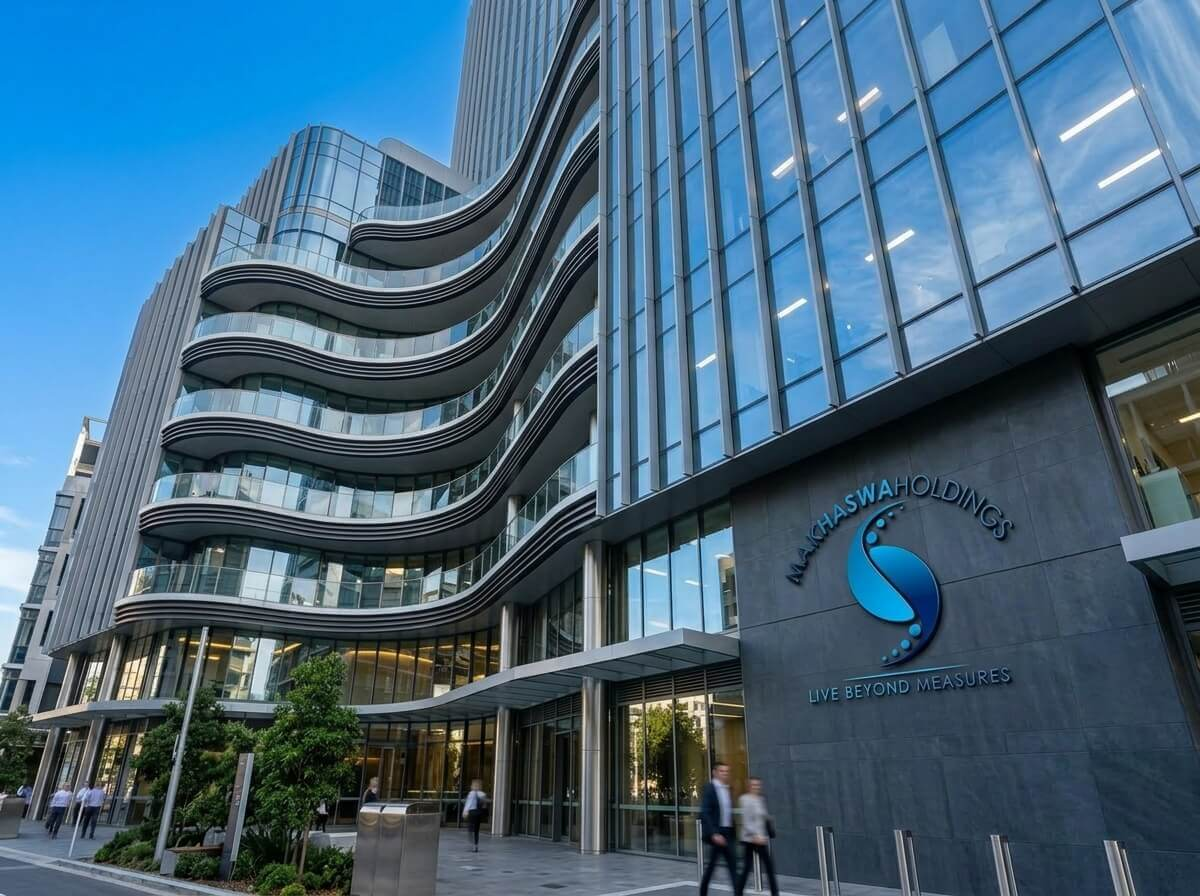
\includegraphics[width=0.48\paperwidth, height=\paperheight, keepaspectratio=false]{images/makhaswa-building-hero.jpeg}
    };

    % Small Right Page Number
    \node[anchor=south east, inner sep=0pt] at ([xshift=-0.8cm, yshift=0.8cm]current page.south east) {
        {\fontsize{9pt}{10pt}\selectfont\bfseries\color{white}2}
    };
\end{tikzpicture}
\clearpage
\setcounter{page}{3}

% --- END corporate/02-contents.tex ---

% --- BEGIN corporate/03-executive-overview.tex ---
% =========================================================================
% PAGE 3 --- EXECUTIVE SUMMARY & NATIONAL FOOTPRINT
% =========================================================================
\phantomsection\hypertarget{sec:overview}{}\pdfbookmark[1]{01. Executive Overview \& Footprint}{sec:overview}
\sectionbanner{EXECUTIVE OVERVIEW}{Corporate Identity, Strategic Vision \& National Footprint}

\noindent
\begin{minipage}[t]{0.62\textwidth}
    {\large\bfseries\color{mhnavy} Who We Are}
    \vspace{0.12cm}

    {\fontsize{9.0pt}{13.0pt}\selectfont\color{mhtext}
    \textbf{Makhaswa Holdings (Pty) Ltd} is a 100\% Black-Owned, Level 1 B-BBEE multi-disciplinary civil engineering, infrastructure development, mechanical, and general building construction enterprise headquartered in Pretoria, Gauteng. The company was officially incorporated with the Companies and Intellectual Property Commission (CIPC) on \textbf{17 July 2017} (Registration: \textbf{2017/307900/07}).
    }

    \vspace{0.22cm}

    {\fontsize{9.0pt}{13.0pt}\selectfont\color{mhtext}
    Through disciplined project delivery and continuous technical investment, Makhaswa Holdings has expanded its operational capacity, holding active accreditations in \textbf{CIDB Grade 8 CE PE} (Civil Engineering) and \textbf{8 ME PE} (Mechanical Engineering), alongside Specialist Building (\textbf{7SB PE}), Electrical Infrastructure (\textbf{7EB PE}), and General Building (\textbf{6GB PE}).
    }

    \vspace{0.22cm}

    {\fontsize{9.0pt}{13.0pt}\selectfont\color{mhtext}
    We execute public infrastructure tenders, municipal framework contracts, commercial facilities, and bulk reticulation schemes across Gauteng, Limpopo, KwaZulu-Natal, and North West.
    }
\end{minipage}
\hfill
\begin{minipage}[t]{0.34\textwidth}
    % Credentials Stat Container
    \begin{tcolorbox}[
        enhanced,
        colback=mhoffwhite,
        colframe=mhnavy,
        boxrule=1pt,
        arc=4pt,
        title={\bfseries\color{white}\faAward\ Key Accreditations},
        colbacktitle=mhnavy,
        left=7pt, right=7pt, top=6pt, bottom=6pt,
        drop shadow=black!6
    ]
        \fontsize{8.2pt}{11.8pt}\selectfont
        \textcolor{mhnavy}{\rule{4pt}{4pt}}\hspace{4pt}\textbf{CIDB Grade 8 CE PE / 8 ME PE}\\
        \textcolor{mhnavy}{\rule{4pt}{4pt}}\hspace{4pt}\textbf{CIDB 7SB PE / 7EB PE / 6GB PE}\\
        \textcolor{mhnavy}{\rule{4pt}{4pt}}\hspace{4pt}\textbf{Level 1 B-BBEE (135\% Recognition)}\\
        \textcolor{mhnavy}{\rule{4pt}{4pt}}\hspace{4pt}\textbf{NHBRC Registered (Class 5 Builder)}\\
        \textcolor{mhnavy}{\rule{4pt}{4pt}}\hspace{4pt}\textbf{ISO 9001 $\bullet$ 14001 $\bullet$ 45001 Aligned}
    \end{tcolorbox}

    \vspace{0.25cm}

    \begin{tcolorbox}[
        enhanced, colback=white, colframe=mhlightgray, boxrule=0.8pt, arc=4pt,
        left=6pt, right=6pt, top=6pt, bottom=6pt, halign=center,
        drop shadow=black!4
    ]
        {\fontsize{18pt}{20pt}\selectfont\bfseries\color{mhblue} 2017}\\[1pt]
        {\fontsize{7.5pt}{9pt}\selectfont\color{mhtextmuted}\MakeUppercase{Incorporated July 2017}}\\[4pt]
        \textcolor{mhlightgray}{\rule{3.2cm}{0.6pt}}\\[4pt]
        {\fontsize{18pt}{20pt}\selectfont\bfseries\color{mhblue} 100\%}\\[1pt]
        {\fontsize{7.5pt}{9pt}\selectfont\color{mhtextmuted}\MakeUppercase{Black Owned / 50\% Female}}
    \end{tcolorbox}
\end{minipage}

\vfill

% Vision & Mission Split Cards
\noindent
\begin{minipage}[t]{0.485\textwidth}
    \begin{tcolorbox}[
        enhanced, colback=white, colframe=mhlightgray, boxrule=0.8pt, arc=4pt,
        title={\bfseries\color{white}\faEye\ Our Vision},
        colbacktitle=mhnavy, fonttitle=\bfseries\small,
        left=8pt, right=8pt, top=8pt, bottom=8pt,
        drop shadow=black!4
    ]
        {\fontsize{8.6pt}{12.2pt}\selectfont\color{mhtext}
        To be a leading African infrastructure and engineering contractor recognized for execution excellence, innovative engineering solutions, uncompromised safety standards, and sustainable socio-economic development.
        }
    \end{tcolorbox}
\end{minipage}
\hfill
\begin{minipage}[t]{0.485\textwidth}
    \begin{tcolorbox}[
        enhanced, colback=white, colframe=mhlightgray, boxrule=0.8pt, arc=4pt,
        title={\bfseries\color{white}\faBullseye\ Our Mission},
        colbacktitle=mhblue, fonttitle=\bfseries\small,
        left=8pt, right=8pt, top=8pt, bottom=8pt,
        drop shadow=black!4
    ]
        {\fontsize{8.6pt}{12.2pt}\selectfont\color{mhtext}
        Delivering durable, cost-effective, and high-quality civil and mechanical infrastructure on schedule and within budget, while empowering host communities through local employment, skills transfer, and contractor development.
        }
    \end{tcolorbox}
\end{minipage}

\vfill

% National Footprint Operations Directory (4 Regional Hubs)
{\large\bfseries\color{mhnavy} National Footprint \& Strategic Operating Centers}
\vspace{0.10cm}

\noindent
\begin{minipage}[t]{0.235\textwidth}
    \begin{tcolorbox}[enhanced, colback=mhoffwhite, colframe=mhlightgray, boxrule=0.8pt, arc=4pt, left=4pt, right=4pt, top=5pt, bottom=5pt, halign=center, drop shadow=black!3]
        {\fontsize{7.8pt}{9.2pt}\selectfont\bfseries\color{mhnavy}\faBuilding\ Pretoria (HQ)}\\[2pt]
        {\fontsize{6.8pt}{8.8pt}\selectfont\color{mhtext}869 Patryshond Street, Garsfontein, Pretoria, 0042\\[2pt]
        \faPhoneAlt\ \href{tel:0129441702}{012 944 1702}}
    \end{tcolorbox}
\end{minipage}\hfill
\begin{minipage}[t]{0.235\textwidth}
    \begin{tcolorbox}[enhanced, colback=mhoffwhite, colframe=mhlightgray, boxrule=0.8pt, arc=4pt, left=4pt, right=4pt, top=5pt, bottom=5pt, halign=center, drop shadow=black!3]
        {\fontsize{7.8pt}{9.2pt}\selectfont\bfseries\color{mhnavy}\faTruckMonster\ Midrand Ops}\\[2pt]
        {\fontsize{6.8pt}{8.8pt}\selectfont\color{mhtext}Midrand Logistics \& Operations Hub, Gauteng\\[2pt]
        \faPhone\ \href{tel:0115680938}{011 568 0938}}
    \end{tcolorbox}
\end{minipage}\hfill
\begin{minipage}[t]{0.235\textwidth}
    \begin{tcolorbox}[enhanced, colback=mhoffwhite, colframe=mhlightgray, boxrule=0.8pt, arc=4pt, left=4pt, right=4pt, top=5pt, bottom=5pt, halign=center, drop shadow=black!3]
        {\fontsize{7.8pt}{9.2pt}\selectfont\bfseries\color{mhnavy}\faHardHat\ Limpopo Hub}\\[2pt]
        {\fontsize{6.8pt}{8.8pt}\selectfont\color{mhtext}197 Dudu Madisha Drive, Chroompark, Mokopane, 0656\\[2pt]
        \faPhoneAlt\ \href{tel:0129441702}{012 944 1702}}
    \end{tcolorbox}
\end{minipage}\hfill
\begin{minipage}[t]{0.235\textwidth}
    \begin{tcolorbox}[enhanced, colback=mhoffwhite, colframe=mhlightgray, boxrule=0.8pt, arc=4pt, left=4pt, right=4pt, top=5pt, bottom=5pt, halign=center, drop shadow=black!3]
        {\fontsize{7.8pt}{9.2pt}\selectfont\bfseries\color{mhnavy}\faMapMarkerAlt\ Durban Hub}\\[2pt]
        {\fontsize{6.8pt}{8.8pt}\selectfont\color{mhtext}71 Bertha Mkhize Street, Durban Central, KZN, 4001\\[2pt]
        \faPhoneAlt\ \href{tel:0129441702}{012 944 1702}}
    \end{tcolorbox}
\end{minipage}

\clearpage

% --- END corporate/03-executive-overview.tex ---

% --- BEGIN corporate/04-leadership.tex ---
% =========================================================================
% PAGE 4 --- GOVERNANCE, LEADERSHIP & CORPORATE ORGANOGRAM
% =========================================================================
\phantomsection\hypertarget{sec:leadership}{}\pdfbookmark[1]{02. Governance \& Leadership}{sec:leadership}
\enlargethispage{2.5cm}
\sectionbanner{GOVERNANCE \& LEADERSHIP}{Executive Management, Organogram \& Statutory Appointments}

\noindent
\begin{minipage}[t]{0.485\textwidth}
    \begin{tcolorbox}[
        enhanced, colback=white, colframe=mhlightgray, boxrule=0.8pt, arc=4pt,
        left=8pt, right=8pt, top=7pt, bottom=7pt,
        borderline west={3.5pt}{0pt}{mhnavy}, drop shadow=black!4
    ]
        {\fontsize{10.0pt}{12pt}\selectfont\bfseries\color{mhnavy}Lucas Dinga} \ \ {\fontsize{7.8pt}{9.5pt}\selectfont\color{mhtextmuted}(CEO / Authorized Signatory)}\\[2pt]
        {\fontsize{7.6pt}{9.5pt}\selectfont\bfseries\color{mhblue}\faUserTie\ Statutory CR 7(19c) Appointee}\\[2.5pt]
        {\fontsize{8.2pt}{11.0pt}\selectfont\color{mhtext}
        Oversees corporate strategy, commercial expansion, tender procurement, joint ventures, and client relations. Brings over 10 years of specialised experience in civil engineering, road works, and major building contracts. Sole designated signatory for legal contracts and financial operations.
        }
    \end{tcolorbox}
\end{minipage}
\hfill
\begin{minipage}[t]{0.485\textwidth}
    \begin{tcolorbox}[
        enhanced, colback=white, colframe=mhlightgray, boxrule=0.8pt, arc=4pt,
        left=8pt, right=8pt, top=7pt, bottom=7pt,
        borderline west={3.5pt}{0pt}{mhblue}, drop shadow=black!4
    ]
        {\fontsize{10.0pt}{12pt}\selectfont\bfseries\color{mhnavy}Nelly Motswapong (Ms. Nelly)} \ \ {\fontsize{7.8pt}{9.5pt}\selectfont\color{mhtextmuted}(Director / Co-Owner)}\\[2pt]
        {\fontsize{7.6pt}{9.5pt}\selectfont\bfseries\color{mhblue}\faUserShield\ 50\% Black Female Ownership Equity}\\[2.5pt]
        {\fontsize{8.2pt}{11.0pt}\selectfont\color{mhtext}
        Directs corporate governance, human capital development, broad-based enterprise transformation, CSI initiatives, and operational administration. Ensures that all site operations adhere strictly to employment equity and community upliftment mandates.
        }
    \end{tcolorbox}
\end{minipage}

\vspace{0.18cm}

{\large\bfseries\color{mhnavy} Statutory Appointments (OHS Act 85 of 1993 \& Construction Regulations 2014)}
\vspace{0.08cm}

\noindent
\renewcommand{\arraystretch}{1.18}
\begin{tabularx}{\textwidth}{@{}p{3.8cm} p{3.4cm} p{2.2cm} X@{}}
\rowcolor{mhnavy}
{\color{white}\bfseries\fontsize{8pt}{9.8pt}\selectfont Key Personnel} &
{\color{white}\bfseries\fontsize{8pt}{9.8pt}\selectfont Designation} &
{\color{white}\bfseries\fontsize{8pt}{9.8pt}\selectfont Statutory Ref} &
{\color{white}\bfseries\fontsize{8pt}{9.8pt}\selectfont Primary Operational Responsibility} \\
\rowcolor{mhbluelight}
\fontsize{7.6pt}{9.5pt}\selectfont\bfseries Lucas Dinga & \fontsize{7.6pt}{9.5pt}\selectfont Chief Executive Officer & \fontsize{7.6pt}{9.5pt}\selectfont CR 7(19c) & \fontsize{7.6pt}{9.5pt}\selectfont Corporate leadership, commercial sign-off, tender bids \\
\fontsize{7.6pt}{9.5pt}\selectfont\bfseries Elphas Goodman Mdaka & \fontsize{7.6pt}{9.5pt}\selectfont Project \& Contracts Manager & \fontsize{7.6pt}{9.5pt}\selectfont CR 16.2 \& 8.1 & \fontsize{7.6pt}{9.5pt}\selectfont Contractual administration, client liaison (\href{tel:0744810520}{074 481 0520}) \\
\rowcolor{mhbluelight}
\fontsize{7.6pt}{9.5pt}\selectfont\bfseries Sfiso Knowledge Nkabinde & \fontsize{7.6pt}{9.5pt}\selectfont Construction Manager / Site Agent & \fontsize{7.6pt}{9.5pt}\selectfont CR 8.1 & \fontsize{7.6pt}{9.5pt}\selectfont Day-to-day site management, resource execution \\
\fontsize{7.6pt}{9.5pt}\selectfont\bfseries Lindelani Shangase & \fontsize{7.6pt}{9.5pt}\selectfont SHEQ Officer & \fontsize{7.6pt}{9.5pt}\selectfont CR 8.5 (Pr.OHS) & \fontsize{7.6pt}{9.5pt}\selectfont Health \& Safety audits, environmental compliance \\
\rowcolor{mhbluelight}
\fontsize{7.6pt}{9.5pt}\selectfont\bfseries Hendrick Chauke & \fontsize{7.6pt}{9.5pt}\selectfont Quality Controller (QC) & \fontsize{7.6pt}{9.5pt}\selectfont CR 8.38 & \fontsize{7.6pt}{9.5pt}\selectfont ITPs, slump tests, concrete 28-day cube crushing \\
\fontsize{7.6pt}{9.5pt}\selectfont\bfseries Henry Chauke & \fontsize{7.6pt}{9.5pt}\selectfont Section Supervisor & \fontsize{7.6pt}{9.5pt}\selectfont CR 8.8 & \fontsize{7.6pt}{9.5pt}\selectfont Section layerworks, pipelaying, structural builds \\
\rowcolor{mhbluelight}
\fontsize{7.6pt}{9.5pt}\selectfont\bfseries C. Mazarura & \fontsize{7.6pt}{9.5pt}\selectfont Professional Land Surveyor & \fontsize{7.6pt}{9.5pt}\selectfont Pr.L.S. & \fontsize{7.6pt}{9.5pt}\selectfont Setting out, GPS road profiling, as-built coordinates \\
\end{tabularx}
\renewcommand{\arraystretch}{1}

\vspace{0.20cm}
\nopagebreak

% =========================================================================
% HIGH-END TIKZ CORPORATE ORGANIZATIONAL & SITE SUPERVISORY STRUCTURE
% =========================================================================
\noindent
\begin{tcolorbox}[
    enhanced, colback=white, colframe=mhlightgray, boxrule=0.8pt, arc=4pt,
    left=6pt, right=6pt, top=7pt, bottom=7pt, drop shadow=black!4
]
    \centering
    {\fontsize{9.2pt}{11.2pt}\selectfont\bfseries\color{mhnavy}\faSitemap\ \ Corporate Organizational \& Site Supervisory Structure}\\[6pt]
    \begin{tikzpicture}[
        scale=1.0, transform shape,
        topbox/.style={
            rectangle, draw=mhnavy, fill=mhnavy, rounded corners=3.5pt,
            font=\fontsize{7.6pt}{9.2pt}\selectfont\bfseries, align=center, inner sep=4.5pt, text=white,
            line width=0.9pt, drop shadow={opacity=0.15, shadow xshift=0.5pt, shadow yshift=-0.5pt}
        },
        midbox/.style={
            rectangle, draw=mhnavy2, fill=mhnavy2, rounded corners=3.5pt,
            font=\fontsize{7.4pt}{9.0pt}\selectfont\bfseries, align=center, inner sep=4.0pt, text=white,
            line width=0.8pt, drop shadow={opacity=0.12, shadow xshift=0.5pt, shadow yshift=-0.5pt}
        },
        pillbox/.style={
            rectangle, draw=mhnavy3, fill=mhbluelight!70, rounded corners=3.5pt,
            font=\fontsize{7.0pt}{8.4pt}\selectfont, align=center, inner sep=3.8pt, text=mhnavy,
            line width=0.8pt, drop shadow={opacity=0.08, shadow xshift=0.4pt, shadow yshift=-0.4pt}
        },
        subpillbox/.style={
            rectangle, draw=mhnavy3!70, fill=white, rounded corners=3.5pt,
            font=\fontsize{6.8pt}{8.2pt}\selectfont, align=center, inner sep=3.6pt, text=mhnavy,
            line width=0.7pt
        },
        botbox/.style={
            rectangle, draw=mhnavy, fill=mhbluelight!90, rounded corners=3.5pt,
            font=\fontsize{7.2pt}{8.8pt}\selectfont\bfseries, align=center, inner sep=4.5pt, text=mhnavy,
            line width=0.9pt, drop shadow={opacity=0.10, shadow xshift=0.5pt, shadow yshift=-0.5pt}
        },
        busline/.style={draw=mhnavy3, line width=1.0pt},
        arrline/.style={draw=mhnavy3, -{Stealth[length=4.0pt, width=3.2pt]}, line width=0.9pt}
    ]
        % Level 1: Board & Executive Leadership
        \node[topbox, text width=12.8cm] (exec) at (0, 0) {
            {\color{mhgold}\faCrown}\ \ \textbf{Board of Directors \& Executive Leadership}\\[1.5pt]
            {\normalfont\fontsize{6.8pt}{8.0pt}\selectfont Lucas Dinga \textbf{(CEO / CR 7(19c) Designated Signatory)} \ $\bullet$ \ Nelly Motswapong \textbf{(Director / Co-Owner)}}
        };

        % Level 2: Contracts & Project Management
        \node[midbox, text width=10.8cm] (cm) at (0, -1.18) {
            \faBriefcase\ \ \textbf{Contracts, Project \& Construction Management (CR 16.2 / 8.1)}\\[1.5pt]
            {\normalfont\fontsize{6.8pt}{8.0pt}\selectfont Elphas Goodman Mdaka \textbf{(Contracts Mgr)}}
        };
        \draw[arrline] (exec.south) -- (cm.north);

        % Level 3: Three Operational Pillars (Symmetrical: -5.7cm, 0.0cm, +5.7cm)
        \node[pillbox, text width=5.25cm] (site) at (-5.7, -2.75) {
            \textbf{\color{mhnavy}\faHardHat\ Site Execution \& Delivery}\\[2pt]
            {\fontsize{6.6pt}{7.8pt}\selectfont\textbf{Sfiso Knowledge Nkabinde} (CR 8.1)\\Construction Manager / Site Agent}
        };

        \node[pillbox, text width=5.25cm] (sheq) at (0, -2.75) {
            \textbf{\color{mhnavy}\faShieldAlt\ SHEQ Governance \& QC Lab}\\[2pt]
            {\fontsize{6.6pt}{7.8pt}\selectfont\textbf{Lindelani Shangase} (CR 8.5 Pr.OHS)\\
            \textbf{Hendrick Chauke} (CR 8.38 QC Testing)}
        };

        \node[pillbox, text width=5.25cm] (surv) at (5.7, -2.75) {
            \textbf{\color{mhnavy}\faDraftingCompass\ Survey \& Geomatics}\\[2pt]
            {\fontsize{6.6pt}{7.8pt}\selectfont\textbf{C. Mazarura} (Pr.L.S.)\\
            Setting Out, GPS Profiling \& As-Builts}
        };

        % Level 2 to Level 3 Connector Bus
        \coordinate (busL2) at (0, -1.85);
        \draw[busline] (cm.south) -- (busL2);
        \draw[busline] (-5.7, -1.85) -- (5.7, -1.85);
        \draw[arrline] (-5.7, -1.85) -- (site.north);
        \draw[arrline] (0, -1.85) -- (sheq.north);
        \draw[arrline] (5.7, -1.85) -- (surv.north);

        % Level 4: Section Supervision Tier
        \node[subpillbox, text width=5.25cm] (subsite) at (-5.7, -4.35) {
            \textbf{\color{mhnavy}\faUsersCog\ Section Supervisors (CR 8.8)}\\[1.8pt]
            {\fontsize{6.5pt}{7.6pt}\selectfont\textbf{Henry Chauke} (Section Supervisor)\\Pipelaying, Layerworks \& Structures}
        };

        \node[subpillbox, text width=5.25cm] (subsheq) at (0, -4.35) {
            \textbf{\color{mhnavy}\faClipboardCheck\ Site Safety \& Lab Sampling}\\[1.8pt]
            {\fontsize{6.5pt}{7.6pt}\selectfont Daily Toolbox Talks $\bullet$ Troxler Density\\Cube Crushing \& Slump Verification}
        };

        \node[subpillbox, text width=5.25cm] (subsurv) at (5.7, -4.35) {
            \textbf{\color{mhnavy}\faMapMarkedAlt\ Field Setting Out}\\[1.8pt]
            {\fontsize{6.5pt}{7.6pt}\selectfont Leica / Topcon Total Station Teams\\Precision Grade Pegging \& Inverts}
        };

        \draw[arrline] (site.south) -- (subsite.north);
        \draw[arrline] (sheq.south) -- (subsheq.north);
        \draw[arrline] (surv.south) -- (subsurv.north);

        % Level 5: Direct Execution \& Community Workforce
        \node[botbox, text width=17.2cm] (workforce) at (0, -6.00) {
            \faTools\ \ \textbf{Site Operations, Certified Trades \& Host Community Labour Force}\\[1.5pt]
            {\normalfont\fontsize{6.6pt}{7.8pt}\selectfont\textbf{Certified Heavy Machine Operators} (Excavators, Graders, Rollers, TLBs, Pavers) \ $\bullet$ \ \textbf{Skilled Artisans} (Pipefitters, Welders, Steel-fixers, Bricklayers) \ $\bullet$ \ \textbf{Local Community Labour (100--200 Personnel)} (30\%--50\% LED Target)}
        };

        % Connectors to bottom box
        \coordinate (busL4) at (0, -5.20);
        \draw[busline] (subsite.south) -- (-5.7, -5.20);
        \draw[busline] (subsheq.south) -- (0, -5.20);
        \draw[busline] (subsurv.south) -- (5.7, -5.20);
        \draw[busline] (-5.7, -5.20) -- (5.7, -5.20);
        \draw[arrline] (0, -5.20) -- (workforce.north);
    \end{tikzpicture}
\end{tcolorbox}

\clearpage

% --- END corporate/04-leadership.tex ---

% --- BEGIN corporate/05-accreditations.tex ---
% =========================================================================
% PAGE 5 --- STATUTORY REGISTRATIONS, ACCREDITATIONS & CIDB MATRIX
% =========================================================================
\phantomsection\hypertarget{sec:accreditations}{}\pdfbookmark[1]{03. Accreditations \& Statutory Matrix}{sec:accreditations}
\sectionbanner{ACCREDITATIONS}{CIDB Grading Matrix, Statutory Registrations \& Banking}

\noindent
\begin{minipage}[t]{0.62\textwidth}
    {\large\bfseries\color{mhnavy} CIDB Contractor Registration Credentials}
    \vspace{0.10cm}

    {\fontsize{8.8pt}{12.4pt}\selectfont\color{mhtext}
    Makhaswa Holdings is registered with the Construction Industry Development Board (\textbf{CIDB}) under Contractor Registration Number (\textbf{CRS}): \textbf{10153817}. Our multi-disciplinary gradings enable independent tendering and joint venture participation on major public and private infrastructure schemes:
    }

    \vspace{0.15cm}

    \renewcommand{\arraystretch}{1.25}
    \begin{tabularx}{\linewidth}{@{}l c p{3.6cm} r@{}}
    \rowcolor{mhnavy}
    {\color{white}\bfseries\fontsize{7.6pt}{9.2pt}\selectfont Grade} & {\color{white}\bfseries\fontsize{7.6pt}{9.2pt}\selectfont Status} & {\color{white}\bfseries\fontsize{7.6pt}{9.2pt}\selectfont Class of Construction} & {\color{white}\bfseries\fontsize{7.6pt}{9.2pt}\selectfont Tender Limit} \\
    \rowcolor{mhbluelight}
    \fontsize{7.5pt}{9.2pt}\selectfont\bfseries 8 CE PE & \fontsize{7.5pt}{9.2pt}\selectfont Active & \fontsize{7.5pt}{9.2pt}\selectfont Civil Engineering & \fontsize{7.5pt}{9.2pt}\selectfont\bfseries Up to R200M+ \\
    \fontsize{7.5pt}{9.2pt}\selectfont\bfseries 8 ME PE & \fontsize{7.5pt}{9.2pt}\selectfont Active & \fontsize{7.5pt}{9.2pt}\selectfont Mechanical Engineering & \fontsize{7.5pt}{9.2pt}\selectfont\bfseries Up to R200M+ \\
    \rowcolor{mhbluelight}
    \fontsize{7.5pt}{9.2pt}\selectfont\bfseries 7 SB PE & \fontsize{7.5pt}{9.2pt}\selectfont Active & \fontsize{7.5pt}{9.2pt}\selectfont Specialist Building Works & \fontsize{7.5pt}{9.2pt}\selectfont\bfseries Up to R60M \\
    \fontsize{7.5pt}{9.2pt}\selectfont\bfseries 7 EB PE & \fontsize{7.5pt}{9.2pt}\selectfont Active & \fontsize{7.5pt}{9.2pt}\selectfont Electrical Infrastructure & \fontsize{7.5pt}{9.2pt}\selectfont\bfseries Up to R60M \\
    \rowcolor{mhbluelight}
    \fontsize{7.5pt}{9.2pt}\selectfont\bfseries 6 GB PE & \fontsize{7.5pt}{9.2pt}\selectfont Active & \fontsize{7.5pt}{9.2pt}\selectfont General Building & \fontsize{7.5pt}{9.2pt}\selectfont\bfseries Up to R20M \\
    \end{tabularx}
    \renewcommand{\arraystretch}{1}
\end{minipage}
\hfill
\begin{minipage}[t]{0.34\textwidth}
    \begin{tcolorbox}[
        enhanced, colback=white, colframe=mhlightgray, boxrule=0.8pt, arc=4pt,
        title={\bfseries\color{white}\faBuilding\ NHBRC Registration},
        colbacktitle=mhnavy, fonttitle=\bfseries\small,
        left=7pt, right=7pt, top=6pt, bottom=6pt,
        drop shadow=black!4
    ]
        {\fontsize{7.8pt}{10.8pt}\selectfont\color{mhtext}
        \textbf{Registration No:} 4000006217\\
        \textbf{Category:} General Home Builder\\
        \textbf{Grading:} Class 5 Certified\\
        Enables delivery of government housing developments, GAP schemes, and turnkey commercial residential cluster projects.
        }
    \end{tcolorbox}

    \vspace{0.20cm}

    \begin{tcolorbox}[
        enhanced, colback=mhoffwhite, colframe=mhnavy, boxrule=0.8pt, arc=4pt,
        title={\bfseries\color{white}\faAward\ B-BBEE Credentials},
        colbacktitle=mhnavy, fonttitle=\bfseries\small,
        left=7pt, right=7pt, top=6pt, bottom=6pt,
        drop shadow=black!4
    ]
        {\fontsize{7.8pt}{10.8pt}\selectfont\color{mhtext}
        \textbf{Rating:} Level 1 Contributor\\
        \textbf{Procurement Recognition:} 135\%\\
        \textbf{Black Ownership:} 100\%\\
        \textbf{Black Female Ownership:} 50\%\\
        \textbf{Empowering Supplier:} Yes
        }
    \end{tcolorbox}
\end{minipage}

\vfill

{\large\bfseries\color{mhnavy} Statutory Compliance \& Verified Banking Details}
\vspace{0.08cm}

\noindent
\begin{minipage}[t]{0.485\textwidth}
    \begin{tcolorbox}[enhanced, colback=white, colframe=mhlightgray, boxrule=0.8pt, arc=4pt, left=8pt, right=8pt, top=7pt, bottom=7pt, drop shadow=black!3]
        {\fontsize{8.5pt}{11pt}\selectfont\bfseries\color{mhnavy}\faFileContract\ Corporate Statutory Registrations}\\[3pt]
        {\fontsize{7.8pt}{11.0pt}\selectfont\color{mhtext}
        \textbf{CIPC Company Registration:} 2017/307900/07\\
        \textbf{SARS Tax Reference Number:} 9670117176\\
        \textbf{SARS VAT Registration Number:} 4840286027\\
        \textbf{SARS TCS PIN:} Compliant (Tax Status Valid)\\
        \textbf{COIDA / W.C. Registration:} 990001402241 (Good Standing)\\
        \textbf{CSD Supplier Number:} MAAA0513997 (Verified Tender Vendor)
        }
    \end{tcolorbox}
\end{minipage}
\hfill
\begin{minipage}[t]{0.485\textwidth}
    \begin{tcolorbox}[enhanced, colback=white, colframe=mhlightgray, boxrule=0.8pt, arc=4pt, left=8pt, right=8pt, top=7pt, bottom=7pt, drop shadow=black!3]
        {\fontsize{8.5pt}{11pt}\selectfont\bfseries\color{mhnavy}\faUniversity\ Official Verified Banking Details}\\[3pt]
        {\fontsize{7.8pt}{11.0pt}\selectfont\color{mhtext}
        \textbf{Banking Institution:} First National Bank (FNB)\\
        \textbf{Account Holder:} Makhaswa Holdings (Pty) Ltd\\
        \textbf{Account Type:} Commercial / Corporate Cheque\\
        \textbf{Account Number:} 62896570997\\
        \textbf{Branch Name / Code:} Corporate Core / 250655\\
        \textbf{Guarantees \& Facilities:} Commercial Performance Guarantees via FNB \& Approved Financial Guarantors
        }
    \end{tcolorbox}
\end{minipage}

\vfill

% Compliance Logo Strip (4 Logos)
\noindent
\begin{minipage}[t]{0.235\textwidth}
    \begin{tcolorbox}[enhanced, colback=white, colframe=mhlightgray, boxrule=0.7pt, arc=4pt, left=2pt, right=2pt, top=4pt, bottom=4pt, halign=center, drop shadow=black!3]
        
\includegraphics[height=1.0cm, keepaspectratio]{images/cidb-logo.png}\\[2pt]
        {\fontsize{7.0pt}{8.0pt}\selectfont\bfseries\color{mhnavy}CIDB Grade 8 CE / 8 ME}
    \end{tcolorbox}
\end{minipage}\hfill
\begin{minipage}[t]{0.235\textwidth}
    \begin{tcolorbox}[enhanced, colback=white, colframe=mhlightgray, boxrule=0.7pt, arc=4pt, left=2pt, right=2pt, top=4pt, bottom=4pt, halign=center, drop shadow=black!3]
        
\includegraphics[height=1.0cm, keepaspectratio]{images/bbbee-logo.png}\\[2pt]
        {\fontsize{7.0pt}{8.0pt}\selectfont\bfseries\color{mhnavy}Level 1 B-BBEE (135\%)}
    \end{tcolorbox}
\end{minipage}\hfill
\begin{minipage}[t]{0.235\textwidth}
    \begin{tcolorbox}[enhanced, colback=white, colframe=mhlightgray, boxrule=0.7pt, arc=4pt, left=2pt, right=2pt, top=4pt, bottom=4pt, halign=center, drop shadow=black!3]
        
\includegraphics[height=1.0cm, keepaspectratio]{images/nhbrc-logo.png}\\[2pt]
        {\fontsize{7.0pt}{8.0pt}\selectfont\bfseries\color{mhnavy}NHBRC Class 5 Builder}
    \end{tcolorbox}
\end{minipage}\hfill
\begin{minipage}[t]{0.235\textwidth}
    \begin{tcolorbox}[enhanced, colback=white, colframe=mhlightgray, boxrule=0.7pt, arc=4pt, left=2pt, right=2pt, top=4pt, bottom=4pt, halign=center, drop shadow=black!3]
        
\includegraphics[height=1.0cm, keepaspectratio]{images/iso-logo.png}\\[2pt]
        {\fontsize{7.0pt}{8.0pt}\selectfont\bfseries\color{mhnavy}ISO 9001 / 14001 / 45001}
    \end{tcolorbox}
\end{minipage}

\clearpage

% --- END corporate/05-accreditations.tex ---

% --- BEGIN corporate/06-journey.tex ---
% =========================================================================
% PAGE 6 --- OUR JOURNEY (KEY MILESTONES & STRATEGIC TRAJECTORY)
% =========================================================================
\phantomsection\hypertarget{sec:journey}{}\pdfbookmark[1]{04. Our Journey \& Milestones}{sec:journey}
\sectionbanner{OUR JOURNEY}{Strategic Growth, Key Milestones \& Track Record}

\noindent
\begin{minipage}[t]{0.62\textwidth}
    {\large\bfseries\color{mhnavy} A Trajectory of Disciplined Scaling}
    \vspace{0.12cm}

    {\fontsize{9.0pt}{13.0pt}\selectfont\color{mhtext}
    Since its incorporation in \textbf{July 2017}, Makhaswa Holdings has followed a calculated, capital-reinvestment trajectory. Beginning with municipal road maintenance and civil subcontracts in Gauteng, the enterprise progressively acquired heavy yellow metal, upgraded technical staff competencies, and systematically scaled its CIDB grading profile.
    }

    \vspace{0.20cm}

    {\fontsize{9.0pt}{13.0pt}\selectfont\color{mhtext}
    Today, Makhaswa operates as an established contractor holding \textbf{CIDB 8 CE PE} and \textbf{8 ME PE}, executing infrastructure frameworks across Gauteng, Limpopo, KwaZulu-Natal, and North West under strict technical and quality standards.
    }
\end{minipage}
\hfill
\begin{minipage}[t]{0.34\textwidth}
    \statcard{mhblue}{R200M+}{Tender Capacity per Project}
    \vspace{0.20cm}
    \statcard{mhnavy}{17+}{Completed Infrastructure Contracts}
\end{minipage}

\vfill

{\large\bfseries\color{mhnavy} Strategic Milestones Timeline (2017 --- 2026)}
\vspace{0.10cm}

\noindent
\begin{tcolorbox}[enhanced, colback=white, colframe=mhlightgray, boxrule=0.8pt, arc=4pt, left=6pt, right=6pt, top=8pt, bottom=8pt, drop shadow=black!4]
    \centering
    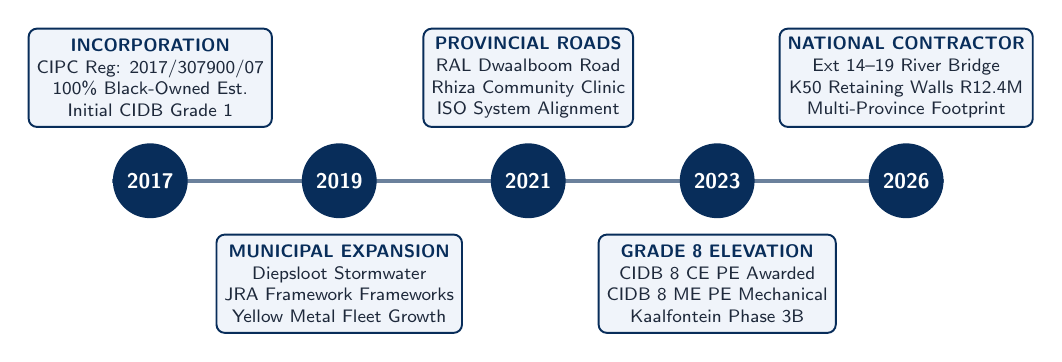
\begin{tikzpicture}[
        scale=0.96, transform shape,
        mstone/.style={rectangle, draw=mhnavy, fill=mhbluelight, text=mhtext, rounded corners=3pt, minimum width=2.6cm, minimum height=1.3cm, align=center, font=\fontsize{6.8pt}{8.2pt}\selectfont, inner sep=3pt, line width=0.7pt},
        yr/.style={circle, draw=mhnavy, fill=mhnavy, text=white, font=\fontsize{8pt}{9pt}\selectfont\bfseries, minimum size=0.9cm, line width=1pt},
        line/.style={draw=mhnavy!60, line width=1.5pt}
    ]
        \coordinate (y1) at (-5.0, 0);
        \coordinate (y2) at (-2.5, 0);
        \coordinate (y3) at (0.0, 0);
        \coordinate (y4) at (2.5, 0);
        \coordinate (y5) at (5.0, 0);

        \draw[line] (-5.5, 0) -- (5.5, 0);

        \node[yr] (c1) at (y1) {2017};
        \node[yr] (c2) at (y2) {2019};
        \node[yr] (c3) at (y3) {2021};
        \node[yr] (c4) at (y4) {2023};
        \node[yr] (c5) at (y5) {2026};

        \node[mstone, anchor=south] at (-5.0, 0.7) {%
            \bfseries\color{mhnavy}INCORPORATION\\%
            CIPC Reg: 2017/307900/07\\%
            100\% Black-Owned Est.\\%
            Initial CIDB Grade 1%
        };

        \node[mstone, anchor=north] at (-2.5, -0.7) {%
            \bfseries\color{mhnavy}MUNICIPAL EXPANSION\\%
            Diepsloot Stormwater\\%
            JRA Framework Frameworks\\%
            Yellow Metal Fleet Growth%
        };

        \node[mstone, anchor=south] at (0.0, 0.7) {%
            \bfseries\color{mhnavy}PROVINCIAL ROADS\\%
            RAL Dwaalboom Road\\%
            Rhiza Community Clinic\\%
            ISO System Alignment%
        };

        \node[mstone, anchor=north] at (2.5, -0.7) {%
            \bfseries\color{mhnavy}GRADE 8 ELEVATION\\%
            CIDB 8 CE PE Awarded\\%
            CIDB 8 ME PE Mechanical\\%
            Kaalfontein Phase 3B%
        };

        \node[mstone, anchor=south] at (5.0, 0.7) {%
            \bfseries\color{mhnavy}NATIONAL CONTRACTOR\\%
            Ext 14--19 River Bridge\\%
            K50 Retaining Walls R12.4M\\%
            Multi-Province Footprint%
        };
    \end{tikzpicture}
\end{tcolorbox}

\vfill

{\large\bfseries\color{mhnavy} Key Growth Metrics}
\vspace{0.10cm}

\noindent
\begin{minipage}[t]{0.235\textwidth}\iconstatcard{mhnavy}{100\%}{Black Owned}{\faAward}\end{minipage}\hfill
\begin{minipage}[t]{0.235\textwidth}\iconstatcard{mhblue}{50\%}{Female Equity}{\faFemale}\end{minipage}\hfill
\begin{minipage}[t]{0.235\textwidth}\iconstatcard{mhbluebright}{4 Hubs}{Provincial Footprint}{\faMapMarkedAlt}\end{minipage}\hfill
\begin{minipage}[t]{0.235\textwidth}\iconstatcard{mhnavy3}{100\%}{Safety Record}{\faShieldAlt}\end{minipage}

\clearpage

% --- END corporate/06-journey.tex ---

% --- BEGIN corporate/07-services-directory.tex ---
% =========================================================================
% PAGE 7 --- CORE ENGINEERING DISCIPLINES & TECHNICAL SERVICES DIRECTORY
% =========================================================================
\phantomsection\hypertarget{sec:capabilities}{}\pdfbookmark[1]{05. Core Engineering Services Directory}{sec:capabilities}
\sectionbanner{OUR SERVICES}{Master Engineering Disciplines \& Technical Services Directory}

\noindent
{\fontsize{8.8pt}{12.2pt}\selectfont\color{mhtext}
\textbf{Makhaswa Holdings (Pty) Ltd} operates a structured multi-disciplinary engineering model. To provide tender evaluation committees, consulting engineers, and public procurement boards with uncompromised clarity, each of our \textbf{13 technical trades} is detailed in a dedicated 2-page standalone technical chapter with specifications, execution methodologies, and verified project records:
}

\vspace{0.20cm}

\renewcommand{\arraystretch}{1.18}
\begin{tabularx}{\textwidth}{@{}l p{4.2cm} X c@{}}
\rowcolor{mhnavy}
{\color{white}\bfseries\fontsize{7.8pt}{9.2pt}\selectfont No.} & {\color{white}\bfseries\fontsize{7.8pt}{9.2pt}\selectfont Construction Trade Section} & {\color{white}\bfseries\fontsize{7.8pt}{9.2pt}\selectfont Core Technical Scope \& SANS / COLTO Specifications} & {\color{white}\bfseries\fontsize{7.8pt}{9.2pt}\selectfont Chapter} \\
\rowcolor{mhbluelight}
\fontsize{7.5pt}{9.0pt}\selectfont\bfseries 01 & \fontsize{7.5pt}{9.0pt}\selectfont\bfseries Bulk Earthworks \& Site Prep & \fontsize{7.5pt}{9.0pt}\selectfont Mass excavation, cut-to-fill balancing, topsoil stripping, soil stabilisation & \fontsize{7.5pt}{9.0pt}\selectfont\hyperlink{sec:earthworks}{\bfseries\color{mhblue}Pages 9--10} \\
\fontsize{7.5pt}{9.0pt}\selectfont\bfseries 02 & \fontsize{7.5pt}{9.0pt}\selectfont\bfseries Road Construction \& Layerworks & \fontsize{7.5pt}{9.0pt}\selectfont Subgrade prep, dump rock, G7/G5 sub-base, C3/C4 stabilization, G1 base & \fontsize{7.5pt}{9.0pt}\selectfont\hyperlink{sec:roads}{\bfseries\color{mhblue}Pages 11--12} \\
\rowcolor{mhbluelight}
\fontsize{7.5pt}{9.0pt}\selectfont\bfseries 03 & \fontsize{7.5pt}{9.0pt}\selectfont\bfseries Asphalt Surfacing \& Rehab & \fontsize{7.5pt}{9.0pt}\selectfont Continuously graded asphalt, overlays, mill-and-replace inlays, slurry seal & \fontsize{7.5pt}{9.0pt}\selectfont\hyperlink{sec:asphalt}{\bfseries\color{mhblue}Pages 13--14} \\
\fontsize{7.5pt}{9.0pt}\selectfont\bfseries 04 & \fontsize{7.5pt}{9.0pt}\selectfont\bfseries Kerbing, Paving \& Traffic Signals & \fontsize{7.5pt}{9.0pt}\selectfont Precast kerbs, 80mm paving, traffic lights, signal ducting, markings (7EB) & \fontsize{7.5pt}{9.0pt}\selectfont\hyperlink{sec:kerbing}{\bfseries\color{mhblue}Pages 15--16} \\
\rowcolor{mhbluelight}
\fontsize{7.5pt}{9.0pt}\selectfont\bfseries 05 & \fontsize{7.5pt}{9.0pt}\selectfont\bfseries Stormwater Drainage Networks & \fontsize{7.5pt}{9.0pt}\selectfont Concrete pipes 450--1200mm, Ogee culverts, JRA kerb inlets, catchpits & \fontsize{7.5pt}{9.0pt}\selectfont\hyperlink{sec:stormwater}{\bfseries\color{mhblue}Pages 17--18} \\
\fontsize{7.5pt}{9.0pt}\selectfont\bfseries 06 & \fontsize{7.5pt}{9.0pt}\selectfont\bfseries Bridges \& Concrete Retaining Walls & \fontsize{7.5pt}{9.0pt}\selectfont In-situ decks, abutments, box culverts, cantilever RC retaining walls & \fontsize{7.5pt}{9.0pt}\selectfont\hyperlink{sec:bridges}{\bfseries\color{mhblue}Pages 19--20} \\
\rowcolor{mhbluelight}
\fontsize{7.5pt}{9.0pt}\selectfont\bfseries 07 & \fontsize{7.5pt}{9.0pt}\selectfont\bfseries Gabions \& Rock Mattresses & \fontsize{7.5pt}{9.0pt}\selectfont Hexagonal mesh baskets, Reno mattresses, gravity retaining, scour aprons & \fontsize{7.5pt}{9.0pt}\selectfont\hyperlink{sec:gabions}{\bfseries\color{mhblue}Pages 21--22} \\
\fontsize{7.5pt}{9.0pt}\selectfont\bfseries 08 & \fontsize{7.5pt}{9.0pt}\selectfont\bfseries Stone Pitching \& Hydraulic Protection & \fontsize{7.5pt}{9.0pt}\selectfont Dry-packed pitching, mortared pitching, rock rip-rap, stepped energy dissipators & \fontsize{7.5pt}{9.0pt}\selectfont\hyperlink{sec:pitching}{\bfseries\color{mhblue}Pages 23--24} \\
\rowcolor{mhbluelight}
\fontsize{7.5pt}{9.0pt}\selectfont\bfseries 09 & \fontsize{7.5pt}{9.0pt}\selectfont\bfseries Bulk Water \& Potable Reticulation & \fontsize{7.5pt}{9.0pt}\selectfont Bulk supply mains (uPVC/HDPE/Steel), pressure testing, chemical disinfection & \fontsize{7.5pt}{9.0pt}\selectfont\hyperlink{sec:waterretic}{\bfseries\color{mhblue}Pages 25--26} \\
\fontsize{7.5pt}{9.0pt}\selectfont\bfseries 10 & \fontsize{7.5pt}{9.0pt}\selectfont\bfseries Gravity Sewer Reticulation & \fontsize{7.5pt}{9.0pt}\selectfont Outfall mains, structured-wall uPVC, drop manholes, pneumatic air testing & \fontsize{7.5pt}{9.0pt}\selectfont\hyperlink{sec:sewer}{\bfseries\color{mhblue}Pages 27--28} \\
\rowcolor{mhbluelight}
\fontsize{7.5pt}{9.0pt}\selectfont\bfseries 11 & \fontsize{7.5pt}{9.0pt}\selectfont\bfseries Mechanical Systems (CIDB 8 ME) & \fontsize{7.5pt}{9.0pt}\selectfont Booster pump stations, welded steel pipe spools, valves, PRV assemblies & \fontsize{7.5pt}{9.0pt}\selectfont\hyperlink{sec:mechanical}{\bfseries\color{mhblue}Pages 29--30} \\
\fontsize{7.5pt}{9.0pt}\selectfont\bfseries 12 & \fontsize{7.5pt}{9.0pt}\selectfont\bfseries General Building \& Commercial (6GB) & \fontsize{7.5pt}{9.0pt}\selectfont Clinics, schools, commercial facilities, NHBRC Class 5 housing & \fontsize{7.5pt}{9.0pt}\selectfont\hyperlink{sec:building}{\bfseries\color{mhblue}Pages 31--32} \\
\rowcolor{mhbluelight}
\fontsize{7.5pt}{9.0pt}\selectfont\bfseries 13 & \fontsize{7.5pt}{9.0pt}\selectfont\bfseries Electrical Reticulation (CIDB 7 EB) & \fontsize{7.5pt}{9.0pt}\selectfont High-mast lighting poles (20m--30m), cabling, substation civils, palisade & \fontsize{7.5pt}{9.0pt}\selectfont\hyperlink{sec:electrical}{\bfseries\color{mhblue}Pages 33--34} \\
\end{tabularx}
\renewcommand{\arraystretch}{1}

\vfill

{\large\bfseries\color{mhnavy} Five-Stage Project Delivery Methodology}
\vspace{0.10cm}

\noindent
\begin{minipage}[t]{0.185\textwidth}\iconstatcard{mhnavy}{01}{Planning}{\faClipboardList}\end{minipage}\hfill
\begin{minipage}[t]{0.185\textwidth}\iconstatcard{mhblue}{02}{Procurement}{\faShoppingCart}\end{minipage}\hfill
\begin{minipage}[t]{0.185\textwidth}\iconstatcard{mhbluebright}{03}{Execution}{\faHardHat}\end{minipage}\hfill
\begin{minipage}[t]{0.185\textwidth}\iconstatcard{mhnavy3}{04}{QA / QC}{\faCheckDouble}\end{minipage}\hfill
\begin{minipage}[t]{0.185\textwidth}\iconstatcard{mhblue}{05}{Handover}{\faKey}\end{minipage}

\clearpage

% --- END corporate/07-services-directory.tex ---

% --- BEGIN corporate/08-sheq.tex ---
% =========================================================================
% PAGE 8 --- SHEQ POLICY, ISO ALIGNMENT & LAB TESTING
% =========================================================================
\phantomsection\hypertarget{sec:sheq}{}\pdfbookmark[1]{06. SHEQ Framework \& Quality Testing}{sec:sheq}
\sectionbanner{SHEQ FRAMEWORK}{Safety, Health, Environment \& Quality Governance}

\noindent
\begin{minipage}[t]{0.31\textwidth}
    \begin{tcolorbox}[
        enhanced, colback=white, colframe=mhlightgray, boxrule=0.8pt, arc=4pt,
        title={\bfseries\color{white}\faShieldAlt\ Occupational Health \& Safety},
        colbacktitle=mhnavy, fonttitle=\bfseries\small,
        left=8pt, right=8pt, top=8pt, bottom=8pt, height=6.3cm,
        drop shadow=black!4
    ]
        {\fontsize{8.4pt}{11.8pt}\selectfont\color{mhtext}
        \textbf{Zero Harm Commitment:} Strict adherence to the OHS Act (Act 85 of 1993) and Construction Regulations 2014. Mandatory daily toolbox talks, SABS-approved PPE enforcement, appointed SHEQ Officers (Pr.OHS), continuous hazard logs, and full OHS site compliance.
        }
    \end{tcolorbox}
\end{minipage}
\hfill
\begin{minipage}[t]{0.31\textwidth}
    \begin{tcolorbox}[
        enhanced, colback=white, colframe=mhlightgray, boxrule=0.8pt, arc=4pt,
        title={\bfseries\color{white}\faCheckDouble\ Quality Assurance \& Testing},
        colbacktitle=mhblue, fonttitle=\bfseries\small,
        left=8pt, right=8pt, top=8pt, bottom=8pt, height=6.3cm,
        drop shadow=black!4
    ]
        {\fontsize{8.4pt}{11.8pt}\selectfont\color{mhtext}
        \textbf{ISO 9001:2015 Alignment:} Documented Inspection and Test Plans (ITPs). Compaction verification via Troxler nuclear density gauges, concrete slump testing, and 150mm cube sampling with 7-, 14-, and 28-day compression crushing at SANAS-accredited testing laboratories.
        }
    \end{tcolorbox}
\end{minipage}
\hfill
\begin{minipage}[t]{0.31\textwidth}
    \begin{tcolorbox}[
        enhanced, colback=white, colframe=mhlightgray, boxrule=0.8pt, arc=4pt,
        title={\bfseries\color{white}\faLeaf\ Environmental Management},
        colbacktitle=mhbluebright, fonttitle=\bfseries\small,
        left=8pt, right=8pt, top=8pt, bottom=8pt, height=6.3cm,
        drop shadow=black!4
    ]
        {\fontsize{8.4pt}{11.8pt}\selectfont\color{mhtext}
        \textbf{ISO 14001:2015 Alignment:} Proactive silt trapping, runoff control berms, bunded hazardous fuel/chemical storage areas, certified waste disposal, topsoil stripping and stockpiling for complete post-construction landscape rehabilitation.
        }
    \end{tcolorbox}
\end{minipage}

\vfill

% SHEQ Visual Accents
\noindent
\begin{minipage}[t]{0.485\textwidth}
    \begin{tcolorbox}[enhanced, colback=mhoffwhite, colframe=mhlightgray, boxrule=0.7pt, arc=4pt, left=8pt, right=8pt, top=7pt, bottom=7pt, drop shadow=black!3]
        \begin{minipage}[c]{0.28\textwidth}
            
\includegraphics[width=\linewidth, height=1.4cm, keepaspectratio]{images/sheq-logo.png}
        \end{minipage}\hfill
        \begin{minipage}[c]{0.68\textwidth}
            {\fontsize{8.8pt}{11.2pt}\selectfont\bfseries\color{mhnavy}Integrated SHEQ Protocols}\\[2.5pt]
            {\fontsize{7.8pt}{10.2pt}\selectfont\color{mhtextmuted}Daily safety checks, risk logs, and complete site compliance auditing.}
        \end{minipage}
    \end{tcolorbox}
\end{minipage}\hfill
\begin{minipage}[t]{0.485\textwidth}
    \begin{tcolorbox}[enhanced, colback=mhoffwhite, colframe=mhlightgray, boxrule=0.7pt, arc=4pt, left=8pt, right=8pt, top=7pt, bottom=7pt, drop shadow=black!3]
        \begin{minipage}[c]{0.28\textwidth}
            
\includegraphics[width=\linewidth, height=1.4cm, keepaspectratio]{images/iso-logo.png}
        \end{minipage}\hfill
        \begin{minipage}[c]{0.68\textwidth}
            {\fontsize{8.8pt}{11.2pt}\selectfont\bfseries\color{mhnavy}ISO System Framework Alignment}\\[2.5pt]
            {\fontsize{7.8pt}{10.2pt}\selectfont\color{mhtextmuted}ISO 9001 (Quality), ISO 14001 (Environment), ISO 45001 (OH\&S).}
        \end{minipage}
    \end{tcolorbox}
\end{minipage}

\vfill

{\large\bfseries\color{mhnavy} Our SHEQ Commitment in Numbers}
\vspace{0.12cm}

\noindent
\begin{minipage}[t]{0.235\textwidth}\iconstatcard{mhnavy}{ISO 3x}{9001 / 14001 / 45001}{\faAward}\end{minipage}\hfill
\begin{minipage}[t]{0.235\textwidth}\iconstatcard{mhblue}{Zero Harm}{Safety Target}{\faShieldAlt}\end{minipage}\hfill
\begin{minipage}[t]{0.235\textwidth}\iconstatcard{mhbluebright}{OHS Act}{85 of 1993 Compliant}{\faGavel}\end{minipage}\hfill
\begin{minipage}[t]{0.235\textwidth}\iconstatcard{mhnavy3}{Daily}{Toolbox Talks}{\faUsers}\end{minipage}

\clearpage

% --- END corporate/08-sheq.tex ---

% --- BEGIN trades/01-bulk-earthworks.tex ---
% =========================================================================
% TRADE 01 --- BULK EARTHWORKS & SITE PREPARATION (PAGE 1 OF 2)
% =========================================================================
\phantomsection\hypertarget{sec:earthworks}{}\pdfbookmark[1]{Trade 01: Bulk Earthworks}{sec:earthworks}
\sectionbanner{BULK EARTHWORKS}{Mass Excavation, Cut-to-Fill Balancing \& Site Preparation}

\noindent
\begin{minipage}[t]{0.62\textwidth}
    \vspace{0pt}
    {\large\bfseries\color{mhnavy} Bulk Earthworks \& Ground Engineering Capability}
    \vspace{0.12cm}

    {\fontsize{9pt}{13pt}\selectfont\color{mhtext}
    \textbf{Makhaswa Holdings (Pty) Ltd} undertakes bulk earthworks for civil infrastructure, road construction, commercial developments and general building projects. The work includes the excavation, movement, placement and shaping of soil and rock to prepare stable construction platforms, foundations, road formations and service corridors.
    }

    \vspace{0.22cm}

    {\fontsize{9pt}{13pt}\selectfont\color{mhtext}
    Our scope covers mass excavation, cut-to-fill balancing, site clearance, topsoil stripping, soil compaction, ground stabilisation, stockpiling and haulage. Excavated material is assessed for suitable reuse in engineered fill, with surplus and unsuitable material managed in accordance with project requirements.
    }

    \vspace{0.22cm}

    {\fontsize{9pt}{13pt}\selectfont\color{mhtext}
    Earthworks are integrated with road layerworks, stormwater drainage, sewer pipelines and building foundations. Survey levels, fill material, layer thickness and compaction requirements are controlled against the engineer's drawings and specifications.
    }
\end{minipage}
\hfill
\begin{minipage}[t]{0.34\textwidth}
    \vspace{0pt}
    \begin{tcolorbox}[
        enhanced, colback=mhoffwhite, colframe=mhnavy, boxrule=1pt, arc=4pt,
        title={\bfseries\color{white}\faTractor\ Earthworks Scope of Work},
        colbacktitle=mhnavy, left=7pt, right=7pt, top=6pt, bottom=6pt,
        drop shadow=black!6
    ]
        \fontsize{8.1pt}{11.6pt}\selectfont
        \textcolor{mhnavy}{\rule{4pt}{4pt}}\hspace{4pt}\textbf{Mass excavation}\\
        \textcolor{mhnavy}{\rule{4pt}{4pt}}\hspace{4pt}\textbf{Cut-to-fill balancing}\\
        \textcolor{mhnavy}{\rule{4pt}{4pt}}\hspace{4pt}\textbf{Site clearance \& stripping}\\
        \textcolor{mhnavy}{\rule{4pt}{4pt}}\hspace{4pt}\textbf{Compaction \& stabilisation}\\
        \textcolor{mhnavy}{\rule{4pt}{4pt}}\hspace{4pt}\textbf{Bulk platform preparation}\\
        \textcolor{mhnavy}{\rule{4pt}{4pt}}\hspace{4pt}\textbf{Stockpiling \& haulage}\\
        \textcolor{mhnavy}{\rule{4pt}{4pt}}\hspace{4pt}\textbf{Controlled demolition}
    \end{tcolorbox}

    \vspace{0.20cm}

    \begin{tcolorbox}[
        enhanced, colback=white, colframe=mhlightgray, boxrule=0.8pt, arc=4pt,
        left=6pt, right=6pt, top=6pt, bottom=6pt, halign=center,
        drop shadow=black!4
    ]
        {\fontsize{18pt}{20pt}\selectfont\bfseries\color{mhblue}8 CE PE}\\[1pt]
        {\fontsize{7.4pt}{9pt}\selectfont\color{mhtextmuted}\MakeUppercase{CIDB Civil Engineering Grade}}\\[4pt]
        \textcolor{mhlightgray}{\rule{3.2cm}{0.6pt}}\\[4pt]
        {\fontsize{13pt}{15pt}\selectfont\bfseries\color{mhnavy}Mod AASHTO}\\[1pt]
        {\fontsize{7.2pt}{9pt}\selectfont\color{mhtextmuted}\MakeUppercase{Compaction Test Reference}}
    \end{tcolorbox}
\end{minipage}

\vfill

% Photos
\noindent
\begin{minipage}[t]{0.315\textwidth}
    \begin{tcolorbox}[enhanced, colback=white, colframe=mhlightgray, boxrule=0.8pt, arc=4pt, left=0pt, right=0pt, top=0pt, bottom=5pt, drop shadow=black!4]
        \tradeimage{bulk-trenching-earthworks-1.jpeg}{2.8cm}
        \centering\vspace{3pt}
        {\fontsize{8pt}{9.8pt}\selectfont\bfseries\color{mhnavy}Mass Excavation \& Trenching}\\[1pt]
        {\fontsize{7pt}{8.4pt}\selectfont\color{mhtextmuted}Excavation and Subgrade Preparation}
    \end{tcolorbox}
\end{minipage}
\hfill
\begin{minipage}[t]{0.315\textwidth}
    \begin{tcolorbox}[enhanced, colback=white, colframe=mhlightgray, boxrule=0.8pt, arc=4pt, left=0pt, right=0pt, top=0pt, bottom=5pt, drop shadow=black!4]
        \tradeimage{plant-and-equipment-fleet.jpeg}{2.8cm}
        \centering\vspace{3pt}
        {\fontsize{8pt}{9.8pt}\selectfont\bfseries\color{mhnavy}Earthmoving Plant}\\[1pt]
        {\fontsize{7pt}{8.4pt}\selectfont\color{mhtextmuted}Heavy Equipment and Material Handling}
    \end{tcolorbox}
\end{minipage}
\hfill
\begin{minipage}[t]{0.315\textwidth}
    \begin{tcolorbox}[enhanced, colback=white, colframe=mhlightgray, boxrule=0.8pt, arc=4pt, left=0pt, right=0pt, top=0pt, bottom=5pt, drop shadow=black!4]
        \tradeimage{earthworks-surfacing-watertruck.jpeg}{2.8cm}
        \centering\vspace{3pt}
        {\fontsize{8pt}{9.8pt}\selectfont\bfseries\color{mhnavy}Earthworks \& Moisture Control}\\[1pt]
        {\fontsize{7pt}{8.4pt}\selectfont\color{mhtextmuted}Water Truck and Site Operations}
    \end{tcolorbox}
\end{minipage}

\vfill

\noindent
{\large\bfseries\color{mhnavy} Core Earthworks Services}
\vspace{0.10cm}

\noindent
\begin{minipage}[t]{0.485\textwidth}
    \servicecard[\faTractor]{01. Mass Excavation}{Bulk removal of soil and rock for foundation excavations, basement levels, road cuttings and building platforms, to the required lines and levels.}
    \vspace{0.16cm}
    \servicecard[\faBalanceScale]{02. Cut-to-Fill Balancing}{Calculation and distribution of suitable excavated material between cut and fill areas to reduce unnecessary off-site disposal and imported fill.}
    \vspace{0.16cm}
    \servicecard[\faLeaf]{03. Site Clearance \& Topsoil Stripping}{Removal of vegetation, obstructions and unsuitable surface material. Reusable topsoil is separately stockpiled for landscaping or reinstatement.}
\end{minipage}
\hfill
\begin{minipage}[t]{0.485\textwidth}
    \servicecard[\faLayerGroup]{04. Compaction \& Soil Stabilisation}{Placement and compaction of engineered fill in specified layers; lime or cement stabilisation where required by the approved material design.}
    \vspace{0.16cm}
    \servicecard[\faBuilding]{05. Bulk Platform \& Formation Preparation}{Formation of level terraces, industrial and commercial building footprints, road subgrades and earthworks for infrastructure services.}
    \vspace{0.16cm}
    \servicecard[\faTruckMoving]{06. Stockpiling \& Haulage}{Segregation, loading, transport and management of reusable, excess and unsuitable material, including removal to authorised disposal facilities.}
\end{minipage}

\clearpage

% =========================================================================
% TRADE 01 --- BULK EARTHWORKS & SITE PREPARATION (PAGE 2 OF 2)
% =========================================================================
\sectionbanner{EARTHWORKS EXECUTION}{Construction Sequence, Plant Operations \& Quality Control}

\noindent
{\large\bfseries\color{mhnavy} Bulk Earthworks Construction Sequence}
\vspace{0.12cm}

\noindent
\begin{minipage}[t]{0.185\textwidth}\processcard{mhnavy}{Survey}{Set-out \& levels}{\faRulerCombined}\end{minipage}\hfill
\begin{minipage}[t]{0.185\textwidth}\processcard{mhblue}{Clear}{Strip \& stockpile}{\faLeaf}\end{minipage}\hfill
\begin{minipage}[t]{0.185\textwidth}\processcard{mhbluebright}{Excavate}{Cut \& load}{\faTractor}\end{minipage}\hfill
\begin{minipage}[t]{0.185\textwidth}\processcard{mhnavy3}{Place}{Fill \& grade}{\faLayerGroup}\end{minipage}\hfill
\begin{minipage}[t]{0.185\textwidth}\processcard{mhblue}{Test}{Compact \& verify}{\faCheckCircle}\end{minipage}

\vspace{0.20cm}

\noindent
\begin{tcolorbox}[enhanced, colback=mhoffwhite, colframe=mhlightgray, boxrule=0.7pt, arc=4pt, left=9pt, right=9pt, top=7pt, bottom=7pt, borderline west={3pt}{0pt}{mhgold}, drop shadow=black!4]
    {\fontsize{8.1pt}{11.0pt}\selectfont\color{mhtext}
    \textbf{Execution method:} Survey control and site clearance precede excavation. Suitable material is directed to designated fill areas; unsuitable material is separated. Fill is spread, moisture-conditioned where necessary, compacted in specified layers and checked for line, level and required density before acceptance of the next layer.
    }
\end{tcolorbox}

\vfill

\noindent
{\large\bfseries\color{mhnavy} Earthworks Activities \& Technical Controls}
\vspace{0.10cm}

{\fontsize{7.7pt}{9.8pt}\selectfont
\renewcommand{\arraystretch}{1.23}
\noindent
\begin{tabularx}{\textwidth}{@{}p{3.3cm} p{6.6cm} X@{}}
\rowcolor{mhnavy}
{\color{white}\bfseries Work Item} & {\color{white}\bfseries Construction Method} & {\color{white}\bfseries Site Control / Inspection} \\
\rowcolor{mhbluelight}
\bfseries Survey \& setting out & Establish existing ground levels, cut/fill boundaries, excavation limits and finished platform levels & Survey records, benchmarks and level verification \\
\bfseries Clearing \& stripping & Remove vegetation, topsoil and obstructions; segregate and stockpile recoverable topsoil & Approved stripping limits and stockpile locations \\
\rowcolor{mhbluelight}
\bfseries Excavation \& material selection & Excavate soil or rock; assess material suitability for fill and direct loads to designated areas & Excavation profiles, material classification and approved disposal routes \\
\bfseries Fill placement \& compaction & Place approved fill in controlled layers, moisture-condition and compact using appropriate rollers & Layer thickness, density testing and engineer's specified compaction criteria \\
\rowcolor{mhbluelight}
\bfseries Stabilisation \& subgrade & Rip, shape and treat unsuitable ground with lime or cement where prescribed & Approved mix design, treatment depth, levels and density testing \\
\bfseries Controlled demolition & Remove existing structures and concrete obstructions under an approved demolition method; separate reusable rubble where specified & Demolition method, service isolation, waste segregation and disposal documentation \\
\end{tabularx}
\renewcommand{\arraystretch}{1}
}

\vfill

\noindent
\begin{minipage}[t]{0.485\textwidth}
    \begin{tcolorbox}[enhanced, colback=white, colframe=mhlightgray, boxrule=0.8pt, arc=4pt, title={\bfseries\color{white}\faTruckMonster\ Plant \& Material Logistics}, colbacktitle=mhnavy, left=8pt, right=8pt, top=7pt, bottom=7pt, drop shadow=black!4]
        {\fontsize{8.1pt}{11.3pt}\selectfont\color{mhtext}
        Excavators, bulldozers, graders, tipper trucks, water trucks and compaction rollers are selected to suit ground conditions and haul distances. Excavation, stockpiling, loading, haulage and material placement are coordinated to maintain the approved work sequence.
        }
    \end{tcolorbox}
\end{minipage}
\hfill
\begin{minipage}[t]{0.485\textwidth}
    \begin{tcolorbox}[enhanced, colback=white, colframe=mhlightgray, boxrule=0.8pt, arc=4pt, title={\bfseries\color{white}\faClipboardCheck\ Quality \& Survey Control}, colbacktitle=mhblue, left=8pt, right=8pt, top=7pt, bottom=7pt, drop shadow=black!4]
        {\fontsize{8.1pt}{11.3pt}\selectfont\color{mhtext}
        Setting out, as-built levels, material classification and layer compaction are checked against the project specification. In-situ density testing is assessed against the specified \textbf{Modified AASHTO} requirement, with test results recorded in the Inspection and Test Plan.
        }
    \end{tcolorbox}
\end{minipage}

\vspace{0.18cm}

\noindent
\begin{minipage}[t]{0.485\textwidth}
    \begin{tcolorbox}[enhanced, colback=white, colframe=mhlightgray, boxrule=0.8pt, arc=4pt, title={\bfseries\color{white}\faShieldAlt\ Safety \& Environmental Controls}, colbacktitle=mhnavy, left=8pt, right=8pt, top=7pt, bottom=7pt, drop shadow=black!4]
        {\fontsize{8.1pt}{11.3pt}\selectfont\color{mhtext}
        Excavation stability, plant movement, buried services, dust, drainage and erosion are managed through the site risk assessment. Topsoil preservation, runoff protection and lawful disposal of waste material form part of the work method.
        }
    \end{tcolorbox}
\end{minipage}
\hfill
\begin{minipage}[t]{0.485\textwidth}
    \begin{tcolorbox}[enhanced, colback=white, colframe=mhlightgray, boxrule=0.8pt, arc=4pt, title={\bfseries\color{white}\faRoad\ Related Civil Engineering Works}, colbacktitle=mhblue, left=8pt, right=8pt, top=7pt, bottom=7pt, drop shadow=black!4]
        {\fontsize{8.1pt}{11.3pt}\selectfont\color{mhtext}
        Earthworks support road construction, stormwater channels, drainage structures, sewer and bulk service trenches, foundation excavations and general building platforms. Work is sequenced with project management and the relevant civil trades.
        }
    \end{tcolorbox}
\end{minipage}

\vfill

\noindent
\begin{tcolorbox}[enhanced, colback=white, colframe=mhnavy, boxrule=0.8pt, arc=3pt, left=8pt, right=8pt, top=6pt, bottom=6pt, drop shadow=black!3]
    {\fontsize{8pt}{10.6pt}\selectfont\color{mhnavy}\bfseries\faCheckCircle\ Technical requirement:}\quad
    {\fontsize{8pt}{10.6pt}\selectfont\color{mhtext}
    Excavation depths, benching, layer thicknesses, material suitability, stabilisation rates and compaction targets are set by the engineer's drawings, geotechnical recommendations and project specification.
    }
\end{tcolorbox}

\clearpage

% --- END trades/01-bulk-earthworks.tex ---

% --- BEGIN trades/02-roads-layerworks.tex ---
% =========================================================================
% TRADE 02 --- ROAD CONSTRUCTION & LAYERWORKS (PAGE 1 OF 2)
% =========================================================================
\phantomsection\hypertarget{sec:roads}{}\pdfbookmark[1]{Trade 02: Road Construction \& Layerworks}{sec:roads}
\sectionbanner{ROAD LAYERWORKS}{Pavement Formation, Subgrade, Sub-Base \& Base Construction}

\noindent
\begin{minipage}[t]{0.62\textwidth}
    \vspace{0pt}
    {\large\bfseries\color{mhnavy} Engineered Road Layerworks \& Pavement Capacity}
    \vspace{0.12cm}

    {\fontsize{9pt}{13pt}\selectfont\color{mhtext}
    \textbf{Makhaswa Holdings (Pty) Ltd} delivers comprehensive roadbed preparation, pioneer stabilization, and pavement layerworks for national, provincial, and municipal transport corridors. All road construction complies with \textbf{COLTO Standard Specifications for Road and Bridge Works} and the \textbf{TRH4 Structural Design of Flexible Pavements} code.
    }

    \vspace{0.22cm}

    {\fontsize{9pt}{13pt}\selectfont\color{mhtext}
    Our capability spans the full pavement structure: subgrade ripping and compaction to 90\%--93\% Mod AASHTO, imported dump rock pioneer layers for unstable or saturated subgrades, selected natural gravel layers (G7/G5), stabilized cement-treated sub-base layers (C3/C4), and high-density graded crushed stone base courses (G1/G2) compacted up to 102\% Mod AASHTO.
    }

    \vspace{0.22cm}

    {\fontsize{9pt}{13pt}\selectfont\color{mhtext}
    Pavement layers are shaped and graded to strict geometric tolerances using Caterpillar 140K/140H motor graders equipped with precision blade slope controls and checked via independent SANAS-accredited laboratory compaction tests.
    }
\end{minipage}
\hfill
\begin{minipage}[t]{0.34\textwidth}
    \vspace{0pt}
    \begin{tcolorbox}[
        enhanced, colback=mhoffwhite, colframe=mhnavy, boxrule=1pt, arc=4pt,
        title={\bfseries\color{white}\faRoad\ Layerworks Scope of Work},
        colbacktitle=mhnavy, left=7pt, right=7pt, top=6pt, bottom=6pt,
        drop shadow=black!6
    ]
        \fontsize{8.1pt}{11.6pt}\selectfont
        \textcolor{mhnavy}{\rule{4pt}{4pt}}\hspace{4pt}\textbf{Roadbed ripping \& shaping}\\
        \textcolor{mhnavy}{\rule{4pt}{4pt}}\hspace{4pt}\textbf{Imported dump rock pioneer}\\
        \textcolor{mhnavy}{\rule{4pt}{4pt}}\hspace{4pt}\textbf{Selected sub-base (G7/G5)}\\
        \textcolor{mhnavy}{\rule{4pt}{4pt}}\hspace{4pt}\textbf{Stabilized sub-base (C3/C4)}\\
        \textcolor{mhnavy}{\rule{4pt}{4pt}}\hspace{4pt}\textbf{Crushed aggregate base (G1/G2)}\\
        \textcolor{mhnavy}{\rule{4pt}{4pt}}\hspace{4pt}\textbf{Moisture-density control}\\
        \textcolor{mhnavy}{\rule{4pt}{4pt}}\hspace{4pt}\textbf{Geometric \& crown profiling}
    \end{tcolorbox}

    \vspace{0.20cm}

    \begin{tcolorbox}[
        enhanced, colback=white, colframe=mhlightgray, boxrule=0.8pt, arc=4pt,
        left=6pt, right=6pt, top=6pt, bottom=6pt, halign=center,
        drop shadow=black!4
    ]
        {\fontsize{18pt}{20pt}\selectfont\bfseries\color{mhblue}COLTO / TRH4}\\[1pt]
        {\fontsize{7.4pt}{9pt}\selectfont\color{mhtextmuted}\MakeUppercase{South African Road Standard}}\\[4pt]
        \textcolor{mhlightgray}{\rule{3.2cm}{0.6pt}}\\[4pt]
        {\fontsize{13pt}{15pt}\selectfont\bfseries\color{mhnavy}98\% -- 102\%}\\[1pt]
        {\fontsize{7.2pt}{9pt}\selectfont\color{mhtextmuted}\MakeUppercase{Mod AASHTO Base Density}}
    \end{tcolorbox}
\end{minipage}

\vfill

% Photos
\noindent
\begin{minipage}[t]{0.315\textwidth}
    \begin{tcolorbox}[enhanced, colback=white, colframe=mhlightgray, boxrule=0.8pt, arc=4pt, left=0pt, right=0pt, top=0pt, bottom=5pt, drop shadow=black!4]
        \tradeimage{asphalt-photos-1.jpeg}{2.8cm}
        \centering\vspace{3pt}
        {\fontsize{8pt}{9.8pt}\selectfont\bfseries\color{mhnavy}Roads \& Layerworks}\\[1pt]
        {\fontsize{7pt}{8.4pt}\selectfont\color{mhtextmuted}Sub-Base Compaction \& Grading}
    \end{tcolorbox}
\end{minipage}
\hfill
\begin{minipage}[t]{0.315\textwidth}
    \begin{tcolorbox}[enhanced, colback=white, colframe=mhlightgray, boxrule=0.8pt, arc=4pt, left=0pt, right=0pt, top=0pt, bottom=5pt, drop shadow=black!4]
        \tradeimage{earthworks-surfacing-watertruck.jpeg}{2.8cm}
        \centering\vspace{3pt}
        {\fontsize{8pt}{9.8pt}\selectfont\bfseries\color{mhnavy}Moisture Conditioning}\\[1pt]
        {\fontsize{7pt}{8.4pt}\selectfont\color{mhtextmuted}Water Tankers \& Compaction}
    \end{tcolorbox}
\end{minipage}
\hfill
\begin{minipage}[t]{0.315\textwidth}
    \begin{tcolorbox}[enhanced, colback=white, colframe=mhlightgray, boxrule=0.8pt, arc=4pt, left=0pt, right=0pt, top=0pt, bottom=5pt, drop shadow=black!4]
        \tradeimage{plant-and-equipment-fleet.jpeg}{2.8cm}
        \centering\vspace{3pt}
        {\fontsize{8pt}{9.8pt}\selectfont\bfseries\color{mhnavy}Heavy Graders \& Rollers}\\[1pt]
        {\fontsize{7pt}{8.4pt}\selectfont\color{mhtextmuted}Compaction Equipment Fleet}
    \end{tcolorbox}
\end{minipage}

\vfill

\noindent
{\large\bfseries\color{mhnavy} Core Layerworks Services}
\vspace{0.10cm}

\noindent
\begin{minipage}[t]{0.485\textwidth}
    \servicecard[\faRuler]{01. Roadbed Preparation \& Ripping}{Ripping, scarifying, moisture conditioning, and re-compacting in-situ subgrade soils to 90\%--93\% Mod AASHTO to establish a stable foundation.}
    \vspace{0.16cm}
    \servicecard[\faLayerGroup]{02. Pioneer Dump Rock Stabilisation}{Importation and interlocking placement of 150mm--300mm coarse dump rock fill to bridge saturated, marshy, or low-bearing clay roadbed sections.}
    \vspace{0.16cm}
    \servicecard[\faTruckLoading]{03. Selected Natural Gravel Layers (G7/G5)}{Sourcing, dumping, spreading, and vibrating approved gravel layers to specified layer thickness, compacted to 93\%--95\% Mod AASHTO.}
\end{minipage}
\hfill
\begin{minipage}[t]{0.485\textwidth}
    \servicecard[\faCogs]{04. Cement-Stabilised Sub-Base (C3/C4)}{In-situ mixing of approved roadbed cement (CEM II), moisture conditioning, and compaction achieving 1.5--3.0 MPa unconfined compressive strength.}
    \vspace{0.16cm}
    \servicecard[\faRoad]{05. Graded Crushed Stone Base (G1/G2)}{Precision motor-grader spreading of high-density quarried crushed aggregate, followed by vibratory rolling and slushing to 98\%--102\% Mod AASHTO.}
    \vspace{0.16cm}
    \servicecard[\faCrosshairs]{06. Stringline \& Profile Geometric Control}{Continuous survey peg setting out, ensuring exact compliance with designed longitudinal falls, cross-falls, super-elevations, and crowns.}
\end{minipage}

\clearpage

% =========================================================================
% TRADE 02 --- ROAD CONSTRUCTION & LAYERWORKS (PAGE 2 OF 2)
% =========================================================================
\sectionbanner{LAYERWORKS EXECUTION}{Construction Sequence, Compaction Standards \& Quality Testing}

\noindent
{\large\bfseries\color{mhnavy} Road Layerworks Construction Sequence}
\vspace{0.12cm}

\noindent
\begin{minipage}[t]{0.185\textwidth}\processcard{mhnavy}{Rip / Shape}{Subgrade prep}{\faRulerCombined}\end{minipage}\hfill
\begin{minipage}[t]{0.185\textwidth}\processcard{mhblue}{Pioneer}{Dump rock fill}{\faLayerGroup}\end{minipage}\hfill
\begin{minipage}[t]{0.185\textwidth}\processcard{mhbluebright}{Stabilize}{C3/C4 cement}{\faCogs}\end{minipage}\hfill
\begin{minipage}[t]{0.185\textwidth}\processcard{mhnavy3}{Base G1}{Crushed rock}{\faRoad}\end{minipage}\hfill
\begin{minipage}[t]{0.185\textwidth}\processcard{mhblue}{Verify}{Troxler density}{\faCheckCircle}\end{minipage}

\vspace{0.20cm}

\noindent
\begin{tcolorbox}[enhanced, colback=mhoffwhite, colframe=mhlightgray, boxrule=0.7pt, arc=4pt, left=9pt, right=9pt, top=7pt, bottom=7pt, borderline west={3pt}{0pt}{mhgold}, drop shadow=black!4]
    {\fontsize{8.1pt}{11.0pt}\selectfont\color{mhtext}
    \textbf{Execution method:} Subgrade is proof-rolled under loaded 10t tippers. Approved materials are hauled, spread with Caterpillar motor graders, and brought to Optimum Moisture Content (OMC). Compaction proceeds using padfoot rollers on cohesive soils and 10t--12t smooth-drum vibratory rollers on gravel and crushed stone base. Each layer is tested with nuclear gauges and signed off prior to placing the subsequent layer.
    }
\end{tcolorbox}

\vfill

\noindent
{\large\bfseries\color{mhnavy} Layerworks Specifications \& Site Inspection Matrix}
\vspace{0.10cm}

{\fontsize{7.7pt}{9.8pt}\selectfont
\renewcommand{\arraystretch}{1.23}
\noindent
\begin{tabularx}{\textwidth}{@{}p{3.3cm} p{6.6cm} X@{}}
\rowcolor{mhnavy}
{\color{white}\bfseries Layer / Work Item} & {\color{white}\bfseries Construction Method \& Equipment} & {\color{white}\bfseries Quality Standard / Field Control} \\
\rowcolor{mhbluelight}
\bfseries Roadbed preparation & Rip to 150mm depth, remove oversize stones (>65mm), moisture-condition to OMC, compact with heavy roller & 90\%--93\% Mod AASHTO, proof rolling under 10t loaded axle without rutting \\
\bfseries Pioneer dump rock & Place clean, sound quarried rock (100mm--250mm) over soft/wet ground, interlock with grid roller & Visual stability sign-off, zero subgrade displacement under plant loads \\
\rowcolor{mhbluelight}
\bfseries Selected sub-base (G7/G5) & Tip and spread approved natural gravel in layers $\le$150mm compacted thickness, compact with 12t vibratory roller & 93\%--95\% Mod AASHTO, layer thickness verified via stringline level pegs \\
\bfseries Stabilised sub-base (C3/C4) & Spread roadbed cement (3\%--4\%), blend with disc harrow/stabilizer, add water to OMC, compact and water-cure & 95\%--97\% Mod AASHTO, UCS 1.5--3.0 MPa at 7 days, 7-day wet burlap or spray curing \\
\rowcolor{mhbluelight}
\bfseries Crushed stone base (G1/G2) & Dump graded crushed aggregate, shape with motor grader, roll with heavy vibrating rollers, slush and sweep & 98\%--102\% Mod AASHTO, surface tolerance $\pm$5mm under 3m straight-edge \\
\bfseries Geometric \& profile check & Establish benchmarks, verify centerlines, cross-falls (2\%--3\%), super-elevations and kerb interface levels & As-built survey log, level tolerance within $\pm$5mm of design elevations \\
\end{tabularx}
\renewcommand{\arraystretch}{1}
}

\vfill

\noindent
\begin{minipage}[t]{0.485\textwidth}
    \begin{tcolorbox}[enhanced, colback=white, colframe=mhlightgray, boxrule=0.8pt, arc=4pt, title={\bfseries\color{white}\faTruckMonster\ Dedicated Plant Spreads}, colbacktitle=mhnavy, left=8pt, right=8pt, top=7pt, bottom=7pt, drop shadow=black!4]
        {\fontsize{8.1pt}{11.3pt}\selectfont\color{mhtext}
        Operations utilize Caterpillar 140K/140H graders, 10t--12t smooth-drum vibratory rollers, padfoot compactors, 16,000L water tankers, and 10m$^3$--15m$^3$ tipper fleets for uninterrupted material spreading and compaction cycles.
        }
    \end{tcolorbox}
\end{minipage}
\hfill
\begin{minipage}[t]{0.485\textwidth}
    \begin{tcolorbox}[enhanced, colback=white, colframe=mhlightgray, boxrule=0.8pt, arc=4pt, title={\bfseries\color{white}\faClipboardCheck\ Troxler Density Testing}, colbacktitle=mhblue, left=8pt, right=8pt, top=7pt, bottom=7pt, drop shadow=black!4]
        {\fontsize{8.1pt}{11.3pt}\selectfont\color{mhtext}
        Compaction is verified in-situ using calibrated Troxler nuclear density gauges at regular grid intervals. Maximum dry density (MDD) and unconfined compressive strength (UCS) are confirmed by SANAS-accredited testing laboratories.
        }
    \end{tcolorbox}
\end{minipage}

\vspace{0.18cm}

\noindent
\begin{minipage}[t]{0.485\textwidth}
    \begin{tcolorbox}[enhanced, colback=white, colframe=mhlightgray, boxrule=0.8pt, arc=4pt, title={\bfseries\color{white}\faTrafficLight\ Traffic Accommodation \& Safety}, colbacktitle=mhnavy, left=8pt, right=8pt, top=7pt, bottom=7pt, drop shadow=black!4]
        {\fontsize{8.1pt}{11.3pt}\selectfont\color{mhtext}
        All public road construction operates under approved SARTSM Chapter 13 traffic accommodation plans, including delineators, high-visibility flagmen, temporary signage, and dust-suppression water spraying.
        }
    \end{tcolorbox}
\end{minipage}
\hfill
\begin{minipage}[t]{0.485\textwidth}
    \begin{tcolorbox}[enhanced, colback=white, colframe=mhlightgray, boxrule=0.8pt, arc=4pt, title={\bfseries\color{white}\faLink\ Multi-Trade Civil Alignment}, colbacktitle=mhblue, left=8pt, right=8pt, top=7pt, bottom=7pt, drop shadow=black!4]
        {\fontsize{8.1pt}{11.3pt}\selectfont\color{mhtext}
        Layerworks are carefully sequenced with subsoil drainage installation, concrete stormwater pipes, cable duct sleeves, concrete kerbing haunching, and eventual bituminous asphalt surfacing.
        }
    \end{tcolorbox}
\end{minipage}

\vfill

\noindent
\begin{tcolorbox}[enhanced, colback=white, colframe=mhnavy, boxrule=0.8pt, arc=3pt, left=8pt, right=8pt, top=6pt, bottom=6pt, drop shadow=black!3]
    {\fontsize{8pt}{10.6pt}\selectfont\color{mhnavy}\bfseries\faCheckCircle\ Verified Project Delivery:}\quad
    {\fontsize{8pt}{10.6pt}\selectfont\color{mhtext}
    \textbf{JRA Kaalfontein Phase 3B} (Contract JRA/21/157: 1,090m $\times$ 6.1m layerworks with dump rock stabilization) \& \textbf{JRA Diepsloot Ext 06} (C4 stabilized sub-base and G1 base).
    }
\end{tcolorbox}

\clearpage

% --- END trades/02-roads-layerworks.tex ---

% --- BEGIN trades/03-asphalt-surfacing.tex ---
% =========================================================================
% TRADE 03 --- ASPHALT SURFACING & ROAD REHABILITATION (PAGE 1 OF 2)
% =========================================================================
\phantomsection\hypertarget{sec:asphalt}{}\pdfbookmark[1]{Trade 03: Asphalt Surfacing \& Rehab}{sec:asphalt}
\sectionbanner{ASPHALT SURFACING}{Continuous Paving, Overlays, Inlays \& Surface Rehabilitation}

\noindent
\begin{minipage}[t]{0.62\textwidth}
    \vspace{0pt}
    {\large\bfseries\color{mhnavy} Bituminous Surfacing \& Pavement Rehabilitation Capability}
    \vspace{0.12cm}

    {\fontsize{9pt}{13pt}\selectfont\color{mhtext}
    \textbf{Makhaswa Holdings (Pty) Ltd} delivers precision mechanical asphalt paving, structural overlays, mill-and-replace inlays, and preventive bituminous maintenance for national, provincial, and metropolitan arterial routes. All operations conform to \textbf{COLTO Section 4200} (Asphalt Base and Surfacing) and \textbf{Sabita Manual 35} guidelines.
    }

    \vspace{0.22cm}

    {\fontsize{9pt}{13pt}\selectfont\color{mhtext}
    Our surfacing division undertakes continuously-graded medium and fine hot-mix asphalt (HMA) paving, asphalt overlays, deep milling and inlay patching of rutted or cracked pavements, slurry seal applications, and single/double chip-and-spray surface treatments.
    }

    \vspace{0.22cm}

    {\fontsize{9pt}{13pt}\selectfont\color{mhtext}
    Bituminous works are executed using high-capacity tracked mechanical pavers, steel tandem vibratory rollers, and pneumatic tyre rollers (PTR), ensuring optimal binder density, zero segregation, and superior skid resistance.
    }
\end{minipage}
\hfill
\begin{minipage}[t]{0.34\textwidth}
    \vspace{0pt}
    \begin{tcolorbox}[
        enhanced, colback=mhoffwhite, colframe=mhnavy, boxrule=1pt, arc=4pt,
        title={\bfseries\color{white}\faLayerGroup\ Surfacing Scope of Work},
        colbacktitle=mhnavy, left=7pt, right=7pt, top=6pt, bottom=6pt,
        drop shadow=black!6
    ]
        \fontsize{8.1pt}{11.6pt}\selectfont
        \textcolor{mhnavy}{\rule{4pt}{4pt}}\hspace{4pt}\textbf{Continuously-graded asphalt}\\
        \textcolor{mhnavy}{\rule{4pt}{4pt}}\hspace{4pt}\textbf{Mill-and-replace inlays}\\
        \textcolor{mhnavy}{\rule{4pt}{4pt}}\hspace{4pt}\textbf{Structural asphalt overlays}\\
        \textcolor{mhnavy}{\rule{4pt}{4pt}}\hspace{4pt}\textbf{Cold milling \& profiling}\\
        \textcolor{mhnavy}{\rule{4pt}{4pt}}\hspace{4pt}\textbf{Crack routing \& bitumen sealing}\\
        \textcolor{mhnavy}{\rule{4pt}{4pt}}\hspace{4pt}\textbf{Slurry seal applications}\\
        \textcolor{mhnavy}{\rule{4pt}{4pt}}\hspace{4pt}\textbf{Single/double chip-and-spray}
    \end{tcolorbox}

    \vspace{0.20cm}

    \begin{tcolorbox}[
        enhanced, colback=white, colframe=mhlightgray, boxrule=0.8pt, arc=4pt,
        left=6pt, right=6pt, top=6pt, bottom=6pt, halign=center,
        drop shadow=black!4
    ]
        {\fontsize{18pt}{20pt}\selectfont\bfseries\color{mhblue}COLTO 4200}\\[1pt]
        {\fontsize{7.4pt}{9pt}\selectfont\color{mhtextmuted}\MakeUppercase{Asphalt Specifications}}\\[4pt]
        \textcolor{mhlightgray}{\rule{3.2cm}{0.6pt}}\\[4pt]
        {\fontsize{13pt}{15pt}\selectfont\bfseries\color{mhnavy}Sabita Manual 35}\\[1pt]
        {\fontsize{7.2pt}{9pt}\selectfont\color{mhtextmuted}\MakeUppercase{Mix Design Standards}}
    \end{tcolorbox}
\end{minipage}

\vfill

% Photos
\noindent
\begin{minipage}[t]{0.315\textwidth}
    \begin{tcolorbox}[enhanced, colback=white, colframe=mhlightgray, boxrule=0.8pt, arc=4pt, left=0pt, right=0pt, top=0pt, bottom=5pt, drop shadow=black!4]
        \tradeimage{asphalt-photos-2.jpeg}{2.8cm}
        \centering\vspace{3pt}
        {\fontsize{8pt}{9.8pt}\selectfont\bfseries\color{mhnavy}Asphalt Paver in Action}\\[1pt]
        {\fontsize{7pt}{8.4pt}\selectfont\color{mhtextmuted}Mechanical Hot-Mix Laying}
    \end{tcolorbox}
\end{minipage}
\hfill
\begin{minipage}[t]{0.315\textwidth}
    \begin{tcolorbox}[enhanced, colback=white, colframe=mhlightgray, boxrule=0.8pt, arc=4pt, left=0pt, right=0pt, top=0pt, bottom=5pt, drop shadow=black!4]
        \tradeimage{asphalt-photos-1.jpeg}{2.8cm}
        \centering\vspace{3pt}
        {\fontsize{8pt}{9.8pt}\selectfont\bfseries\color{mhnavy}Finished Road Surface}\\[1pt]
        {\fontsize{7pt}{8.4pt}\selectfont\color{mhtextmuted}Compaction \& Texture Audit}
    \end{tcolorbox}
\end{minipage}
\hfill
\begin{minipage}[t]{0.315\textwidth}
    \begin{tcolorbox}[enhanced, colback=white, colframe=mhlightgray, boxrule=0.8pt, arc=4pt, left=0pt, right=0pt, top=0pt, bottom=5pt, drop shadow=black!4]
        \tradeimage{road-roundabout.jpeg}{2.8cm}
        \centering\vspace{3pt}
        {\fontsize{8pt}{9.8pt}\selectfont\bfseries\color{mhnavy}Municipal Roundabout}\\[1pt]
        {\fontsize{7pt}{8.4pt}\selectfont\color{mhtextmuted}Diepsloot Phase 4 Intersection}
    \end{tcolorbox}
\end{minipage}

\vfill

\noindent
{\large\bfseries\color{mhnavy} Core Asphalt Surfacing Services}
\vspace{0.10cm}

\noindent
\begin{minipage}[t]{0.485\textwidth}
    \servicecard[\faRoad]{01. Continuously-Graded Asphalt Paving}{Mechanical laying of 30mm--40mm medium or fine hot-mix asphalt (HMA) utilizing 50/70 or 70/100 penetration bitumen with precision screed control.}
    \vspace{0.16cm}
    \servicecard[\faTools]{02. Mill-and-Replace Inlays}{Precision cold milling of aged, oxidized, or rutted asphalt to 30mm--50mm depth, followed by immediate application of tack coat and replacement with high-stability mix.}
    \vspace{0.16cm}
    \servicecard[\faLayerGroup]{03. Structural Asphalt Overlays}{Application of structural asphalt leveling and wearing courses over existing flexible or rigid pavements to restore ride quality and extend pavement lifespan.}
\end{minipage}
\hfill
\begin{minipage}[t]{0.485\textwidth}
    \servicecard[\faWater]{04. Crack Routing \& Bitumen Sealing}{Mechanical crack routing, compressed hot-air lance cleaning, and high-pressure injection of hot elastomeric polymer-modified bituminous sealant.}
    \vspace{0.16cm}
    \servicecard[\faPaintRoller]{05. Slurry Seal Surface Treatments}{Application of quick-curing anionic or cationic bitumen slurry seal mixes to enrich oxidized pavement surfaces, seal micro-fissures, and restore macro-texture.}
    \vspace{0.16cm}
    \servicecard[\faTachometerAlt]{06. Single \& Double Chip-and-Spray}{Calibrated bitumen distributor spray of hot elastomeric binder, followed by mechanical aggregate chip spreading (13.2mm / 6.7mm) and pneumatic rolling.}
\end{minipage}

\clearpage

% =========================================================================
% TRADE 03 --- ASPHALT SURFACING & ROAD REHABILITATION (PAGE 2 OF 2)
% =========================================================================
\sectionbanner{ASPHALT EXECUTION}{Milling Sequence, Temperature Controls \& Surface Testing}

\noindent
{\large\bfseries\color{mhnavy} Asphalt Paving Construction Sequence}
\vspace{0.12cm}

\noindent
\begin{minipage}[t]{0.185\textwidth}\processcard{mhnavy}{Mill / Sweep}{Surface clean}{\faBroom}\end{minipage}\hfill
\begin{minipage}[t]{0.185\textwidth}\processcard{mhblue}{Tack Coat}{Bitumen spray}{\faSprayCan}\end{minipage}\hfill
\begin{minipage}[t]{0.185\textwidth}\processcard{mhbluebright}{Lay HMA}{Paver screed}{\faRoad}\end{minipage}\hfill
\begin{minipage}[t]{0.185\textwidth}\processcard{mhnavy3}{Compact}{Steel \& PTR}{\faTruckMonster}\end{minipage}\hfill
\begin{minipage}[t]{0.185\textwidth}\processcard{mhblue}{Audit}{Texture \& cores}{\faCheckCircle}\end{minipage}

\vspace{0.20cm}

\noindent
\begin{tcolorbox}[enhanced, colback=mhoffwhite, colframe=mhlightgray, boxrule=0.7pt, arc=4pt, left=9pt, right=9pt, top=7pt, bottom=7pt, borderline west={3pt}{0pt}{mhgold}, drop shadow=black!4]
    {\fontsize{8.1pt}{11.0pt}\selectfont\color{mhtext}
    \textbf{Execution method:} The milled or base surface is thoroughly swept with mechanical rotary brooms. A 60\% cationic stable-grade bitumen tack coat is applied via calibrated spray bar at 0.55 L/m$^2$. Hot-mix asphalt is delivered at 135$^\circ$C--160$^\circ$C, laid with electronic grade sensors, and compacted immediately: breakdown rolling with 10t--12t tandem steel rollers, followed by intermediate rolling with 15t pneumatic tyre rollers (PTR) to achieve zero visible air voids and tight joint finishes.
    }
\end{tcolorbox}

\vfill

\noindent
{\large\bfseries\color{mhnavy} Surfacing Activities \& Technical Quality Controls}
\vspace{0.10cm}

{\fontsize{7.7pt}{9.8pt}\selectfont
\renewcommand{\arraystretch}{1.23}
\noindent
\begin{tabularx}{\textwidth}{@{}p{3.3cm} p{6.6cm} X@{}}
\rowcolor{mhnavy}
{\color{white}\bfseries Surfacing Activity} & {\color{white}\bfseries Construction Method \& Fleet Operations} & {\color{white}\bfseries Quality Control / Specification Target} \\
\rowcolor{mhbluelight}
\bfseries Cold milling \& sweeping & Cold planer milling to 30mm--50mm depth; vacuum sweep to remove all dust, aggregate, and loose binder & Uniform milled texture, straight edge profile, depth checked every 20m \\
\bfseries Prime \& tack coat spray & Calibrated bitumen distributor spray of inverted prime or 60\% cationic emulsion at 0.55 L/m$^2$ & Uniform spray coverage, zero pooling, full emulsion break verified before paving \\
\rowcolor{mhbluelight}
\bfseries Hot-mix asphalt placement & Mechanical tracked paver with heated vibrating screed, ultrasonic ski level sensors, continuous feed & Asphalt delivery temp 135$^\circ$C--160$^\circ$C, continuous non-stop paver forward travel \\
\bfseries Breakdown \& PTR rolling & Primary pass with 10t--12t steel tandem roller; secondary compaction with 15t pneumatic tyre roller (PTR) & Void content 3\%--6\%, bulk relative density (BRD) verified via laboratory core testing \\
\rowcolor{mhbluelight}
\bfseries Joint construction & Vertical joint cutting along cold edges; paint joint face with hot bitumen prior to placing fresh mix & Seamless, dense longitudinal and transverse joints; tolerance $\pm$3mm under straight-edge \\
\bfseries Crack routing \& sealing & Route cracks to 10mm $\times$ 10mm, blast clean with hot compressed air lance, inject polymer sealant & Full joint penetration, flush elastomeric finish, zero pull-out under traffic \\
\end{tabularx}
\renewcommand{\arraystretch}{1}
}

\vfill

\noindent
\begin{minipage}[t]{0.485\textwidth}
    \begin{tcolorbox}[enhanced, colback=white, colframe=mhlightgray, boxrule=0.8pt, arc=4pt, title={\bfseries\color{white}\faTruckMonster\ Surfacing Plant Logistics}, colbacktitle=mhnavy, left=8pt, right=8pt, top=7pt, bottom=7pt, drop shadow=black!4]
        {\fontsize{8.1pt}{11.3pt}\selectfont\color{mhtext}
        Mechanical tracked pavers, insulated asphalt tippers, 10t--12t tandem vibratory rollers, 15t pneumatic tyre rollers (PTR), and crack-routing rigs ensure continuous hot-feed operations.
        }
    \end{tcolorbox}
\end{minipage}
\hfill
\begin{minipage}[t]{0.485\textwidth}
    \begin{tcolorbox}[enhanced, colback=white, colframe=mhlightgray, boxrule=0.8pt, arc=4pt, title={\bfseries\color{white}\faFlask\ Laboratory Mix Verification}, colbacktitle=mhblue, left=8pt, right=8pt, top=7pt, bottom=7pt, drop shadow=black!4]
        {\fontsize{8.1pt}{11.3pt}\selectfont\color{mhtext}
        Asphalt mix designs comply with Sabita Manual 35. SANAS-accredited core sampling verifies Marshall stability, flow, binder content, void ratios, and skid resistance.
        }
    \end{tcolorbox}
\end{minipage}

\vspace{0.18cm}

\noindent
\begin{minipage}[t]{0.485\textwidth}
    \begin{tcolorbox}[enhanced, colback=white, colframe=mhlightgray, boxrule=0.8pt, arc=4pt, title={\bfseries\color{white}\faThermometerHalf\ Thermal \& Site Safety Control}, colbacktitle=mhnavy, left=8pt, right=8pt, top=7pt, bottom=7pt, drop shadow=black!4]
        {\fontsize{8.1pt}{11.3pt}\selectfont\color{mhtext}
        Infrared temperature monitoring at delivery and screed lay-down prevents cold-rolling defects. Traffic accommodation flagmen and delineators safeguard live lanes.
        }
    \end{tcolorbox}
\end{minipage}
\hfill
\begin{minipage}[t]{0.485\textwidth}
    \begin{tcolorbox}[enhanced, colback=white, colframe=mhlightgray, boxrule=0.8pt, arc=4pt, title={\bfseries\color{white}\faRoad\ Interfaced Civil Road Scope}, colbacktitle=mhblue, left=8pt, right=8pt, top=7pt, bottom=7pt, drop shadow=black!4]
        {\fontsize{8.1pt}{11.3pt}\selectfont\color{mhtext}
        Surfacing interfaces directly with precast concrete kerbing lips, stormwater kerb inlets, bridge expansion joints, thermoplastic markings, and road signage.
        }
    \end{tcolorbox}
\end{minipage}

\vfill

\noindent
\begin{tcolorbox}[enhanced, colback=white, colframe=mhnavy, boxrule=0.8pt, arc=3pt, left=8pt, right=8pt, top=6pt, bottom=6pt, drop shadow=black!3]
    {\fontsize{8pt}{10.6pt}\selectfont\color{mhnavy}\bfseries\faCheckCircle\ Verified Surfacing Delivery:}\quad
    {\fontsize{8pt}{10.6pt}\selectfont\color{mhtext}
    \textbf{RAL Road D2702 Dwaalboom} (Contract RAL/T1171/2021: heavy asphalt overlays, crack routing, and bitumen sealing) \& \textbf{Gauteng DRT23/05/2016} (cold milling, asphalt patching, and surfacing).
    }
\end{tcolorbox}

\clearpage

% --- END trades/03-asphalt-surfacing.tex ---

% --- BEGIN trades/04-kerbing-traffic-signals.tex ---
% =========================================================================
% TRADE 04 --- KERBING, PAVING & TRAFFIC SIGNALIZATION (PAGE 1 OF 2)
% =========================================================================
\phantomsection\hypertarget{sec:kerbing}{}\pdfbookmark[1]{Trade 04: Kerbing, Paving \& Signals}{sec:kerbing}
\sectionbanner{KERBING, PAVING \& SIGNALS}{Precast Kerbs, Interlocking Blocks, Traffic Lights \& Ancillaries}

\noindent
\begin{minipage}[t]{0.62\textwidth}
    \vspace{0pt}
    {\large\bfseries\color{mhnavy} Road Finishing, Interlocking Paving \& Signal Infrastructure}
    \vspace{0.12cm}

    {\fontsize{9pt}{13pt}\selectfont\color{mhtext}
    \textbf{Makhaswa Holdings (Pty) Ltd} delivers turnkey road finishing, pedestrian pathways, heavy-duty interlocking block paving, and intersection traffic signalization infrastructure. Makhaswa holds active accreditations in \textbf{CIDB Grade 8 CE PE} and \textbf{CIDB Grade 7 EB PE} (Electrical Infrastructure), providing verified capability for civil road finishing, service ducting, and electrical reticulation.
    }

    \vspace{0.22cm}

    {\fontsize{9pt}{13pt}\selectfont\color{mhtext}
    Our scope encompasses machine and manual laying of precast concrete kerbing (Figure 3, 7, 8, 8C, and 12), cast-in-situ concrete haunching and channeling, 60mm/80mm Class SA interlocking paving blocks, complete traffic light signal installations (traffic poles, controller cabinets, push-buttons, loop detectors), retro-reflective thermoplastic markings, and road traffic signage.
    }

    \vspace{0.22cm}

    {\fontsize{9pt}{13pt}\selectfont\color{mhtext}
    All road finishing complies with \textbf{SANS 1200 MM}, \textbf{SANS 1058} (Concrete Paving Blocks), \textbf{SANS 927} (Precast Kerbs), and the \textbf{South African Road Traffic Signs Manual (SARTSM)}.
    }
\end{minipage}
\hfill
\begin{minipage}[t]{0.34\textwidth}
    \vspace{0pt}
    \begin{tcolorbox}[
        enhanced, colback=mhoffwhite, colframe=mhnavy, boxrule=1pt, arc=4pt,
        title={\bfseries\color{white}\faTrafficLight\ Finishing Scope of Work},
        colbacktitle=mhnavy, left=7pt, right=7pt, top=6pt, bottom=6pt,
        drop shadow=black!6
    ]
        \fontsize{8.1pt}{11.6pt}\selectfont
        \textcolor{mhnavy}{\rule{4pt}{4pt}}\hspace{4pt}\textbf{Precast kerbs (Fig 3, 7, 8, 8C, 12)}\\
        \textcolor{mhnavy}{\rule{4pt}{4pt}}\hspace{4pt}\textbf{Interlocking paving (60/80mm)}\\
        \textcolor{mhnavy}{\rule{4pt}{4pt}}\hspace{4pt}\textbf{Traffic signals (traffic lights)}\\
        \textcolor{mhnavy}{\rule{4pt}{4pt}}\hspace{4pt}\textbf{Signal ducting \& cable sleeves}\\
        \textcolor{mhnavy}{\rule{4pt}{4pt}}\hspace{4pt}\textbf{Inductive vehicle loop cutting}\\
        \textcolor{mhnavy}{\rule{4pt}{4pt}}\hspace{4pt}\textbf{Thermoplastic road markings}\\
        \textcolor{mhnavy}{\rule{4pt}{4pt}}\hspace{4pt}\textbf{Signage \& steel guardrails}
    \end{tcolorbox}

    \vspace{0.20cm}

    \begin{tcolorbox}[
        enhanced, colback=white, colframe=mhlightgray, boxrule=0.8pt, arc=4pt,
        left=6pt, right=6pt, top=6pt, bottom=6pt, halign=center,
        drop shadow=black!4
    ]
        {\fontsize{18pt}{20pt}\selectfont\bfseries\color{mhblue}CIDB 7 EB PE}\\[1pt]
        {\fontsize{7.4pt}{9pt}\selectfont\color{mhtextmuted}\MakeUppercase{Electrical Infrastructure}}\\[4pt]
        \textcolor{mhlightgray}{\rule{3.2cm}{0.6pt}}\\[4pt]
        {\fontsize{13pt}{15pt}\selectfont\bfseries\color{mhnavy}SANS 1058 / 927}\\[1pt]
        {\fontsize{7.2pt}{9pt}\selectfont\color{mhtextmuted}\MakeUppercase{Precast Quality Standards}}
    \end{tcolorbox}
\end{minipage}

\vfill

% Photos
\noindent
\begin{minipage}[t]{0.315\textwidth}
    \begin{tcolorbox}[enhanced, colback=white, colframe=mhlightgray, boxrule=0.8pt, arc=4pt, left=0pt, right=0pt, top=0pt, bottom=5pt, drop shadow=black!4]
        \tradeimage{road-roundabout.jpeg}{2.8cm}
        \centering\vspace{3pt}
        {\fontsize{8pt}{9.8pt}\selectfont\bfseries\color{mhnavy}Kerbing \& Traffic Islands}\\[1pt]
        {\fontsize{7pt}{8.4pt}\selectfont\color{mhtextmuted}Precast Kerbs \& Channeling}
    \end{tcolorbox}
\end{minipage}
\hfill
\begin{minipage}[t]{0.315\textwidth}
    \begin{tcolorbox}[enhanced, colback=white, colframe=mhlightgray, boxrule=0.8pt, arc=4pt, left=0pt, right=0pt, top=0pt, bottom=5pt, drop shadow=black!4]
        \tradeimage{palisade-fencing-1.jpeg}{2.8cm}
        \centering\vspace{3pt}
        {\fontsize{8pt}{9.8pt}\selectfont\bfseries\color{mhnavy}Road Ancillaries}\\[1pt]
        {\fontsize{7pt}{8.4pt}\selectfont\color{mhtextmuted}Barriers, Fencing \& Signs}
    \end{tcolorbox}
\end{minipage}
\hfill
\begin{minipage}[t]{0.315\textwidth}
    \begin{tcolorbox}[enhanced, colback=white, colframe=mhlightgray, boxrule=0.8pt, arc=4pt, left=0pt, right=0pt, top=0pt, bottom=5pt, drop shadow=black!4]
        \tradeimage{high-mast-electrical-1.jpeg}{2.8cm}
        \centering\vspace{3pt}
        {\fontsize{8pt}{9.8pt}\selectfont\bfseries\color{mhnavy}Electrical \& Signal Power}\\[1pt]
        {\fontsize{7pt}{8.4pt}\selectfont\color{mhtextmuted}CIDB 7 EB Infrastructure}
    \end{tcolorbox}
\end{minipage}

\vfill

\noindent
{\large\bfseries\color{mhnavy} Core Finishing \& Signalization Services}
\vspace{0.10cm}

\noindent
\begin{minipage}[t]{0.485\textwidth}
    \servicecard[\faRoad]{01. Precast Concrete Kerbing \& Haunching}{Installation of Figure 8 semi-mountable, Figure 8C mountable, Figure 7, and Figure 12 barrier kerbing on 15 MPa concrete bedding with continuous backing haunch.}
    \vspace{0.16cm}
    \servicecard[\faTh]{02. Heavy-Duty Interlocking Block Paving}{Laying of 80mm Class SA interlocking paving blocks for heavy traffic roadways, bus rapid transit bays, and intersections; 60mm for pedestrian sidewalks.}
    \vspace{0.16cm}
    \servicecard[\faTrafficLight]{03. Traffic Signal Installations (Traffic Lights)}{Erection, cabling, and commissioning of intersection traffic signal poles, cantilever mast arms, LED signal heads, and pedestrian signal push-buttons.}
\end{minipage}
\hfill
\begin{minipage}[t]{0.485\textwidth}
    \servicecard[\faBolt]{04. Signalized Ducting \& Inductive Loops}{Trenching, bedding, and laying of 110mm PVC electrical cable sleeves, precast concrete draw boxes, and diamond-saw cutting for vehicle detection loops.}
    \vspace{0.16cm}
    \servicecard[\faPaintRoller]{05. Thermoplastic Retro-Reflective Markings}{Mechanical extrusion and spray application of hot-melt thermoplastic paint with drop-on glass beads for durable road centerlines, lane arrows, and pedestrian crossings.}
    \vspace{0.16cm}
    \servicecard[\faShieldAlt]{06. Road Signs, Studs \& Steel Guardrails}{Erection of SADC-RTSM standard road traffic signs, solar-powered and reflective road studs, and galvanized steel W-beam guardrails with terminal wings.}
\end{minipage}

\clearpage

% =========================================================================
% TRADE 04 --- KERBING, PAVING & TRAFFIC SIGNALIZATION (PAGE 2 OF 2)
% =========================================================================
\sectionbanner{ROAD FINISHING EXECUTION}{Alignment, Paving Compaction, Signal Electrification \& Markings}

\noindent
{\large\bfseries\color{mhnavy} Road Finishing Construction Sequence}
\vspace{0.12cm}

\noindent
\begin{minipage}[t]{0.185\textwidth}\processcard{mhnavy}{Sleeve / Duct}{Electrical sleeves}{\faBolt}\end{minipage}\hfill
\begin{minipage}[t]{0.185\textwidth}\processcard{mhblue}{Kerb / Haunch}{15 MPa concrete}{\faRoad}\end{minipage}\hfill
\begin{minipage}[t]{0.185\textwidth}\processcard{mhbluebright}{Sand Bed}{20mm river sand}{\faLayerGroup}\end{minipage}\hfill
\begin{minipage}[t]{0.185\textwidth}\processcard{mhnavy3}{Pave / Vibrate}{Plate compactor}{\faTh}\end{minipage}\hfill
\begin{minipage}[t]{0.185\textwidth}\processcard{mhblue}{Signals / Mark}{Traffic lights \& paint}{\faTrafficLight}\end{minipage}

\vspace{0.20cm}

\noindent
\begin{tcolorbox}[enhanced, colback=mhoffwhite, colframe=mhlightgray, boxrule=0.7pt, arc=4pt, left=9pt, right=9pt, top=7pt, bottom=7pt, borderline west={3pt}{0pt}{mhgold}, drop shadow=black!4]
    {\fontsize{8.1pt}{11.0pt}\selectfont\color{mhtext}
    \textbf{Execution method:} Electrical service ducting and signal sleeves are installed prior to roadbed closure. Kerbs are set to stringline on a 15 MPa concrete bed with continuous concrete backing haunch. For block paving, a 20mm sharp river sand bedding is screeded uncompacted, blocks laid in herringbone pattern, joint plaster sand broomed into joints, and compacted with a plate compactor equipped with a rubber sole. Traffic signal poles and markings follow roadway completion.
    }
\end{tcolorbox}

\vfill

\noindent
{\large\bfseries\color{mhnavy} Finishing Activities \& Technical Controls}
\vspace{0.10cm}

{\fontsize{7.7pt}{9.8pt}\selectfont
\renewcommand{\arraystretch}{1.23}
\noindent
\begin{tabularx}{\textwidth}{@{}p{3.3cm} p{6.6cm} X@{}}
\rowcolor{mhnavy}
{\color{white}\bfseries Finishing Work Item} & {\color{white}\bfseries Construction Method \& Technical Standard} & {\color{white}\bfseries Site Inspection \& Testing Criteria} \\
\rowcolor{mhbluelight}
\bfseries Precast kerb installation & Set kerbs to stringline on 75mm bed of 15 MPa concrete; cast continuous 15 MPa rear haunch & Line and level tolerance $\pm$3mm, uniform 10mm mortar joints, no cracked units \\
\bfseries Interlocking block paving & Screed 20mm clean river sand (uncompacted); lay 60mm/80mm Class SA blocks in 45$^\circ$/90$^\circ$ herringbone & Pattern straightness verified; no joint creep; edge blocks neatly diamond-sawn \\
\rowcolor{mhbluelight}
\bfseries Paving compaction \& sanding & Broom dry plaster sand across joints; vibrate with heavy rubber-soled plate compactor; re-broom & Full joint sand filling; surface tolerance $\pm$5mm under 3m straight-edge \\
\bfseries Traffic signal ducting & Trench and bed 110mm PVC sleeves $\ge$800mm deep; install precast draw boxes with lockable covers & SABS-approved heavy-duty sleeves, draw-wires installed, air mandrel cleared \\
\rowcolor{mhbluelight}
\bfseries Signal poles \& traffic lights & Cast reinforced concrete plinth with holding-down bolts; erect signal pole; wire LED heads and cabinet & Vertical plumb check, SANS 10142-1 electrical compliance, inductive loop sensitivity tested \\
\bfseries Thermoplastic markings & Apply hot-melt thermoplastic at 200$^\circ$C (2mm--3mm thick); spray drop-on reflective glass beads & Retro-reflectivity audit, line width $\pm$5mm, straightness tolerance $\pm$3mm \\
\end{tabularx}
\renewcommand{\arraystretch}{1}
}

\vfill

\noindent
\begin{minipage}[t]{0.485\textwidth}
    \begin{tcolorbox}[enhanced, colback=white, colframe=mhlightgray, boxrule=0.8pt, arc=4pt, title={\bfseries\color{white}\faTools\ Specialized Finishing Tools}, colbacktitle=mhnavy, left=8pt, right=8pt, top=7pt, bottom=7pt, drop shadow=black!4]
        {\fontsize{8.1pt}{11.3pt}\selectfont\color{mhtext}
        Operations utilize diamond masonry block-saws, polyurethane-soled vibratory plate compactors, thermoplastic extrusion applicators, and core-drilling rigs for precise installation.
        }
    \end{tcolorbox}
\end{minipage}
\hfill
\begin{minipage}[t]{0.485\textwidth}
    \begin{tcolorbox}[enhanced, colback=white, colframe=mhlightgray, boxrule=0.8pt, arc=4pt, title={\bfseries\color{white}\faCheckDouble\ SABS Product Certification}, colbacktitle=mhblue, left=8pt, right=8pt, top=7pt, bottom=7pt, drop shadow=black!4]
        {\fontsize{8.1pt}{11.3pt}\selectfont\color{mhtext}
        Paving blocks comply with SANS 1058 ($\ge$25 MPa for 60mm pedestrian; $\ge$35 MPa for 80mm road blocks). Kerbs comply with SANS 927 transverse strength requirements.
        }
    \end{tcolorbox}
\end{minipage}

\vspace{0.18cm}

\noindent
\begin{minipage}[t]{0.485\textwidth}
    \begin{tcolorbox}[enhanced, colback=white, colframe=mhlightgray, boxrule=0.8pt, arc=4pt, title={\bfseries\color{white}\faHardHat\ Live Intersection Safety}, colbacktitle=mhnavy, left=8pt, right=8pt, top=7pt, bottom=7pt, drop shadow=black!4]
        {\fontsize{8.1pt}{11.3pt}\selectfont\color{mhtext}
        Intersection signal works are coordinated with municipal traffic departments, temporary pedestrian walkways, and approved safety barriers around open electrical trenches.
        }
    \end{tcolorbox}
\end{minipage}
\hfill
\begin{minipage}[t]{0.485\textwidth}
    \begin{tcolorbox}[enhanced, colback=white, colframe=mhlightgray, boxrule=0.8pt, arc=4pt, title={\bfseries\color{white}\faCity\ Municipal Infrastructure Integration}, colbacktitle=mhblue, left=8pt, right=8pt, top=7pt, bottom=7pt, drop shadow=black!4]
        {\fontsize{8.1pt}{11.3pt}\selectfont\color{mhtext}
        Finishing ties seamlessly into stormwater catchpits, disabled pram ramps, bus stop shelters, pedestrian walkways, and municipal power distribution grids.
        }
    \end{tcolorbox}
\end{minipage}

\vfill

\noindent
\begin{tcolorbox}[enhanced, colback=white, colframe=mhnavy, boxrule=0.8pt, arc=3pt, left=8pt, right=8pt, top=6pt, bottom=6pt, drop shadow=black!3]
    {\fontsize{8pt}{10.6pt}\selectfont\color{mhnavy}\bfseries\faCheckCircle\ Verified Road Finishing Delivery:}\quad
    {\fontsize{8pt}{10.6pt}\selectfont\color{mhtext}
    \textbf{JRA Diepsloot Ext 06 / Zeph Mothopeng} (Figure 8 kerbs, catchpits, and 80mm heavy-duty paving) \& \textbf{Gauteng DRT23/05/2016} (concrete bus bays, kerbing, and road markings).
    }
\end{tcolorbox}

\clearpage

% --- END trades/04-kerbing-traffic-signals.tex ---

% --- BEGIN trades/05-stormwater-drainage.tex ---
% =========================================================================
% TRADE 05 --- STORMWATER DRAINAGE & CIVIL INFRASTRUCTURE (PAGE 1 OF 2)
% =========================================================================
\phantomsection\hypertarget{sec:stormwater}{}\pdfbookmark[1]{Trade 05: Stormwater Drainage}{sec:stormwater}
\sectionbanner{STORMWATER DRAINAGE}{Concrete Pipelines, Ogee Culverts, Catchpits \& Subsoil Systems}

\noindent
\begin{minipage}[t]{0.62\textwidth}
    \vspace{0pt}
    {\large\bfseries\color{mhnavy} Municipal Stormwater Drainage \& Pipe Reticulation}
    \vspace{0.12cm}

    {\fontsize{9pt}{13pt}\selectfont\color{mhtext}
    \textbf{Makhaswa Holdings (Pty) Ltd} constructs municipal stormwater reticulation networks, deep drainage infrastructure, stream crossings, and specialized subsoil drainage systems. All civil stormwater works comply strictly with \textbf{SANS 1200 DB} (Earthworks for Pipe Trenches), \textbf{SANS 1200 LE} (Stormwater Drainage), and municipal standard drawings (including JRA-SD-SW-020 to 024).
    }

    \vspace{0.22cm}

    {\fontsize{9pt}{13pt}\selectfont\color{mhtext}
    Our capability includes the trenching, bedding cradle preparation, lowering, laying, jointing, and testing of precast concrete spigot-and-socket pipes (diameters: 450mm to 1200mm), Class 100D interlocking Ogee pipes, precast portal box culverts, in-situ reinforced concrete and engineering brick manholes, and standard municipal kerb inlets.
    }

    \vspace{0.22cm}

    {\fontsize{9pt}{13pt}\selectfont\color{mhtext}
    We also install advanced subsoil drainage networks featuring 110mm and 75mm perforated HDPE pipes enveloped in needle-punched non-woven geotextile filter fabric (bidim) and graded stone filter beds to permanently control roadbed groundwater.
    }
\end{minipage}
\hfill
\begin{minipage}[t]{0.34\textwidth}
    \vspace{0pt}
    \begin{tcolorbox}[
        enhanced, colback=mhoffwhite, colframe=mhnavy, boxrule=1pt, arc=4pt,
        title={\bfseries\color{white}\faWater\ Stormwater Scope of Work},
        colbacktitle=mhnavy, left=7pt, right=7pt, top=6pt, bottom=6pt,
        drop shadow=black!6
    ]
        \fontsize{8.1pt}{11.6pt}\selectfont
        \textcolor{mhnavy}{\rule{4pt}{4pt}}\hspace{4pt}\textbf{Concrete pipes (450mm--1200mm)}\\
        \textcolor{mhnavy}{\rule{4pt}{4pt}}\hspace{4pt}\textbf{Class 100D Ogee culverts}\\
        \textcolor{mhnavy}{\rule{4pt}{4pt}}\hspace{4pt}\textbf{In-situ concrete \& brick manholes}\\
        \textcolor{mhnavy}{\rule{4pt}{4pt}}\hspace{4pt}\textbf{JRA standard kerb inlets}\\
        \textcolor{mhnavy}{\rule{4pt}{4pt}}\hspace{4pt}\textbf{Stepped drop manholes}\\
        \textcolor{mhnavy}{\rule{4pt}{4pt}}\hspace{4pt}\textbf{Perforated subsoil drainage}\\
        \textcolor{mhnavy}{\rule{4pt}{4pt}}\hspace{4pt}\textbf{Outfall chutes \& headwalls}
    \end{tcolorbox}

    \vspace{0.20cm}

    \begin{tcolorbox}[
        enhanced, colback=white, colframe=mhlightgray, boxrule=0.8pt, arc=4pt,
        left=6pt, right=6pt, top=6pt, bottom=6pt, halign=center,
        drop shadow=black!4
    ]
        {\fontsize{18pt}{20pt}\selectfont\bfseries\color{mhblue}SANS 1200 LE}\\[1pt]
        {\fontsize{7.4pt}{9pt}\selectfont\color{mhtextmuted}\MakeUppercase{Stormwater Specification}}\\[4pt]
        \textcolor{mhlightgray}{\rule{3.2cm}{0.6pt}}\\[4pt]
        {\fontsize{13pt}{15pt}\selectfont\bfseries\color{mhnavy}450mm -- 1200mm}\\[1pt]
        {\fontsize{7.2pt}{9pt}\selectfont\color{mhtextmuted}\MakeUppercase{Standard Concrete Pipes}}
    \end{tcolorbox}
\end{minipage}

\vfill

% Photos
\noindent
\begin{minipage}[t]{0.315\textwidth}
    \begin{tcolorbox}[enhanced, colback=white, colframe=mhlightgray, boxrule=0.8pt, arc=4pt, left=0pt, right=0pt, top=0pt, bottom=5pt, drop shadow=black!4]
        \tradeimage{culvert-civil-storm-sewer-pipe.jpeg}{2.8cm}
        \centering\vspace{3pt}
        {\fontsize{8pt}{9.8pt}\selectfont\bfseries\color{mhnavy}Stormwater Pipeline Laying}\\[1pt]
        {\fontsize{7pt}{8.4pt}\selectfont\color{mhtextmuted}Spigot \& Socket Reticulation}
    \end{tcolorbox}
\end{minipage}
\hfill
\begin{minipage}[t]{0.315\textwidth}
    \begin{tcolorbox}[enhanced, colback=white, colframe=mhlightgray, boxrule=0.8pt, arc=4pt, left=0pt, right=0pt, top=0pt, bottom=5pt, drop shadow=black!4]
        \tradeimage{culvert-bridge.jpeg}{2.8cm}
        \centering\vspace{3pt}
        {\fontsize{8pt}{9.8pt}\selectfont\bfseries\color{mhnavy}Ogee Culvert Crossings}\\[1pt]
        {\fontsize{7pt}{8.4pt}\selectfont\color{mhtextmuted}Stream Flow \& Road Bypasses}
    \end{tcolorbox}
\end{minipage}
\hfill
\begin{minipage}[t]{0.315\textwidth}
    \begin{tcolorbox}[enhanced, colback=white, colframe=mhlightgray, boxrule=0.8pt, arc=4pt, left=0pt, right=0pt, top=0pt, bottom=5pt, drop shadow=black!4]
        \tradeimage{bulk-trenching-earthworks-1.jpeg}{2.8cm}
        \centering\vspace{3pt}
        {\fontsize{8pt}{9.8pt}\selectfont\bfseries\color{mhnavy}Deep Trench Shoring}\\[1pt]
        {\fontsize{7pt}{8.4pt}\selectfont\color{mhtextmuted}Excavation \& Laser Alignment}
    \end{tcolorbox}
\end{minipage}

\vfill

\noindent
{\large\bfseries\color{mhnavy} Core Stormwater Drainage Services}
\vspace{0.10cm}

\noindent
\begin{minipage}[t]{0.485\textwidth}
    \servicecard[\faWater]{01. Concrete Pipe Reticulation (450mm--1200mm)}{Precision trenching, granular Class B/C bedding cradle preparation, and laying of spigot-and-socket concrete pipes with rubber ring or mortared joints.}
    \vspace{0.16cm}
    \servicecard[\faArchway]{02. Class 100D Interlocking Ogee Culverts}{Installation of high-load Ogee pipes and precast portal box culverts under heavy traffic road crossings and railway embankments.}
    \vspace{0.16cm}
    \servicecard[\faBuilding]{03. In-Situ Concrete \& Brick Manholes}{Construction of reinforced concrete base slabs, engineering brick chambers, and stepped drop manholes with heavy-duty Type 4A/2A ductile iron covers.}
\end{minipage}
\hfill
\begin{minipage}[t]{0.485\textwidth}
    \servicecard[\faInbox]{04. Standard JRA Kerb Inlets \& Catchpits}{Construction of municipal kerb inlets (drawings JRA-SD-SW-020--024) with precast concrete lintels, de-silting catchpit sumps, and grating frames.}
    \vspace{0.16cm}
    \servicecard[\faFilter]{05. Subsoil Groundwater Drainage Systems}{Installation of 110mm/75mm perforated corrugated HDPE subsoil pipes, wrapped in non-woven bidim geotextile fabric and stone filter bedding.}
    \vspace{0.16cm}
    \servicecard[\faMountain]{06. Headwalls, Wingwalls \& Outfall Chutes}{In-situ reinforced concrete headwalls, energy-dissipating drop structures, and stone-pitched outfall aprons to eliminate embankment scour.}
\end{minipage}

\clearpage

% =========================================================================
% TRADE 05 --- STORMWATER DRAINAGE & CIVIL INFRASTRUCTURE (PAGE 2 OF 2)
% =========================================================================
\sectionbanner{STORMWATER EXECUTION}{Trenching Controls, Pipe Bedding, Hydraulic Gradients \& Safety}

\noindent
{\large\bfseries\color{mhnavy} Stormwater Pipeline Construction Sequence}
\vspace{0.12cm}

\noindent
\begin{minipage}[t]{0.185\textwidth}\processcard{mhnavy}{Trench / Shore}{Laser levels}{\faRulerCombined}\end{minipage}\hfill
\begin{minipage}[t]{0.185\textwidth}\processcard{mhblue}{Bedding Bed}{Class B/C cradle}{\faLayerGroup}\end{minipage}\hfill
\begin{minipage}[t]{0.185\textwidth}\processcard{mhbluebright}{Lower / Joint}{Spigot \& socket}{\faWater}\end{minipage}\hfill
\begin{minipage}[t]{0.185\textwidth}\processcard{mhnavy3}{Chambers}{Manholes \& inlets}{\faBuilding}\end{minipage}\hfill
\begin{minipage}[t]{0.185\textwidth}\processcard{mhblue}{Backfill / Test}{Mandrel \& density}{\faCheckCircle}\end{minipage}

\vspace{0.20cm}

\noindent
\begin{tcolorbox}[enhanced, colback=mhoffwhite, colframe=mhlightgray, boxrule=0.7pt, arc=4pt, left=9pt, right=9pt, top=7pt, bottom=7pt, borderline west={3pt}{0pt}{mhgold}, drop shadow=black!4]
    {\fontsize{8.1pt}{11.0pt}\selectfont\color{mhtext}
    \textbf{Execution method:} Trenches are excavated with 20t--30t tracked excavators using pipe lasers to control invert gradients. In deep or unstable ground, certified steel trench boxes provide shoring. A 100mm selected granular bedding cradle is compacted to 90\% Mod AASHTO. Pipes are lowered with webbed slings, jointed using approved rubber rings, and backfilled with selected material compacted in 150mm layers to prevent pipe ovalization or displacement.
    }
\end{tcolorbox}

\vfill

\noindent
{\large\bfseries\color{mhnavy} Stormwater Technical Specifications \& Field Inspections}
\vspace{0.10cm}

{\fontsize{7.7pt}{9.8pt}\selectfont
\renewcommand{\arraystretch}{1.23}
\noindent
\begin{tabularx}{\textwidth}{@{}p{3.3cm} p{6.6cm} X@{}}
\rowcolor{mhnavy}
{\color{white}\bfseries Stormwater Component} & {\color{white}\bfseries Construction Method \& Technical Standard} & {\color{white}\bfseries Inspection \& Acceptance Criteria} \\
\rowcolor{mhbluelight}
\bfseries Trench excavation \& shoring & Excavate trench to engineered invert levels; install trench shields where depth exceeds 1.5m & Trench width $\le$ pipe OD + 600mm; bottom trimmed flat, free of sharp rock points \\
\bfseries Granular bedding cradle & Place 100mm selected granular material (G7/sand); compact to 90\% Mod AASHTO; form socket recesses & Bedding level checked by pipe laser; socket recesses prevent beam action \\
\rowcolor{mhbluelight}
\bfseries Pipe laying \& jointing & Lower pipes using certified webbed lifting slings; push spigot into socket with rubber seal ring & Invert gradient checked every pipe length; line tolerance $\pm$5mm; zero displaced rings \\
\bfseries In-situ concrete manholes & Cast 20 MPa reinforced concrete base slab; build chamber in solid engineering brick or precast rings & Benching sloped at 1:6 to invert; smooth plaster finish; Type 4A covers seated flush \\
\rowcolor{mhbluelight}
\bfseries JRA kerb inlets \& catchpits & Construct to JRA drawings JRA-SD-SW-020--024; seat precast lintel and ductile iron grid frame & Inlet throat unobstructed; catchpit clean; connection pipe sealed with mortar \\
\bfseries Subsoil drainage installation & Lay perforated 110mm pipe on geotextile bed, surround with 19mm stone, wrap fabric with 200mm overlap & Fabric porosity verified; stone free of fine silt; pipe laid at continuous fall \\
\end{tabularx}
\renewcommand{\arraystretch}{1}
}

\vfill

\noindent
\begin{minipage}[t]{0.485\textwidth}
    \begin{tcolorbox}[enhanced, colback=white, colframe=mhlightgray, boxrule=0.8pt, arc=4pt, title={\bfseries\color{white}\faTruckMonster\ Heavy Trenching Fleet}, colbacktitle=mhnavy, left=8pt, right=8pt, top=7pt, bottom=7pt, drop shadow=black!4]
        {\fontsize{8.1pt}{11.3pt}\selectfont\color{mhtext}
        20t--30t tracked excavators, crane trucks with spreader bars, mobile dewatering pumps, and laser pipe-guidance systems ensure continuous, deep pipeline installation.
        }
    \end{tcolorbox}
\end{minipage}
\hfill
\begin{minipage}[t]{0.485\textwidth}
    \begin{tcolorbox}[enhanced, colback=white, colframe=mhlightgray, boxrule=0.8pt, arc=4pt, title={\bfseries\color{white}\faCheckDouble\ Hydraulic Alignment \& Mandrel}, colbacktitle=mhblue, left=8pt, right=8pt, top=7pt, bottom=7pt, drop shadow=black!4]
        {\fontsize{8.1pt}{11.3pt}\selectfont\color{mhtext}
        Every pipeline run is checked for straightness, fall, and obstruction via mirror and smoke testing. Deflection mandrel testing is performed prior to surface handover.
        }
    \end{tcolorbox}
\end{minipage}

\vspace{0.18cm}

\noindent
\begin{minipage}[t]{0.485\textwidth}
    \begin{tcolorbox}[enhanced, colback=white, colframe=mhlightgray, boxrule=0.8pt, arc=4pt, title={\bfseries\color{white}\faShieldAlt\ Trench Safety Governance}, colbacktitle=mhnavy, left=8pt, right=8pt, top=7pt, bottom=7pt, drop shadow=black!4]
        {\fontsize{8.1pt}{11.3pt}\selectfont\color{mhtext}
        Full compliance with Construction Regulation 13 (Excavations). Daily morning inspections by appointed competent excavation supervisors; ladder egress every 10m.
        }
    \end{tcolorbox}
\end{minipage}
\hfill
\begin{minipage}[t]{0.485\textwidth}
    \begin{tcolorbox}[enhanced, colback=white, colframe=mhlightgray, boxrule=0.8pt, arc=4pt, title={\bfseries\color{white}\faRoad\ Pavement Integration}, colbacktitle=mhblue, left=8pt, right=8pt, top=7pt, bottom=7pt, drop shadow=black!4]
        {\fontsize{8.1pt}{11.3pt}\selectfont\color{mhtext}
        Trench backfill beneath road formations is compacted to 95\% Mod AASHTO to prevent differential pavement settlement along kerb lines and road cross-culverts.
        }
    \end{tcolorbox}
\end{minipage}

\vfill

\noindent
\begin{tcolorbox}[enhanced, colback=white, colframe=mhnavy, boxrule=0.8pt, arc=3pt, left=8pt, right=8pt, top=6pt, bottom=6pt, drop shadow=black!3]
    {\fontsize{8pt}{10.6pt}\selectfont\color{mhnavy}\bfseries\faCheckCircle\ Verified Stormwater Delivery:}\quad
    {\fontsize{8pt}{10.6pt}\selectfont\color{mhtext}
    \textbf{JRA Kaalfontein Phase 3B} (600mm lines and manholes at Reed Fish St), \textbf{JRA Diepsloot Ext 11 Phase 4} (675mm--1200mm pipes), and \textbf{Tanganani Ext 51} (450mm--1050mm pipes).
    }
\end{tcolorbox}

\clearpage

% --- END trades/05-stormwater-drainage.tex ---

% --- BEGIN trades/06-bridges-concrete-retaining.tex ---
% =========================================================================
% TRADE 06 --- BRIDGES, CULVERTS & CONCRETE STRUCTURES (PAGE 1 OF 2)
% =========================================================================
\phantomsection\hypertarget{sec:bridges}{}\pdfbookmark[1]{Trade 06: Bridges \& Concrete Structures}{sec:bridges}
\sectionbanner{BRIDGES \& CONCRETE}{Reinforced Bridges, Portal Box Culverts \& Structural Retaining Walls}

\noindent
\begin{minipage}[t]{0.62\textwidth}
    \vspace{0pt}
    {\large\bfseries\color{mhnavy} Structural Concrete, Bridge Engineering \& Retaining Walls}
    \vspace{0.12cm}

    {\fontsize{9pt}{13pt}\selectfont\color{mhtext}
    \textbf{Makhaswa Holdings (Pty) Ltd} delivers turnkey civil structural concrete works for bridge infrastructure, major river crossings, large-aperture precast portal box culverts, and structural retaining wall systems. Makhaswa holds **CIDB Grade 8 CE PE** (Civil Engineering up to R200M+) and **CIDB 7 SB PE** (Specialist Building Works), backed by extensive bridge reconstruction and structural concrete credentials.
    }

    \vspace{0.22cm}

    {\fontsize{9pt}{13pt}\selectfont\color{mhtext}
    Our capability spans bridge demolition, heavy temporary falsework, rebar fixing, and in-situ reinforced concrete casting for bridge decks, abutments, piers, wingwalls, bridge parapets, and approach slabs to \textbf{TMH7} and \textbf{COLTO Section 6000} standards.
    }

    \vspace{0.22cm}

    {\fontsize{9pt}{13pt}\selectfont\color{mhtext}
    We also engineer and construct **Rigid Reinforced Concrete (RC) Cantilever Retaining Walls** and **Mass Concrete Retaining Walls** up to 6m in height for heavy road embankment stabilization, bridge abutment protection, and cut-to-fill terraces (such as the R12.47M Garstfontein Road K50 Retaining Walls contract).
    }
\end{minipage}
\hfill
\begin{minipage}[t]{0.34\textwidth}
    \vspace{0pt}
    \begin{tcolorbox}[
        enhanced, colback=mhoffwhite, colframe=mhnavy, boxrule=1pt, arc=4pt,
        title={\bfseries\color{white}\faArchway\ Concrete Scope of Work},
        colbacktitle=mhnavy, left=7pt, right=7pt, top=6pt, bottom=6pt,
        drop shadow=black!6
    ]
        \fontsize{8.1pt}{11.6pt}\selectfont
        \textcolor{mhnavy}{\rule{4pt}{4pt}}\hspace{4pt}\textbf{In-situ RC bridge decks}\\
        \textcolor{mhnavy}{\rule{4pt}{4pt}}\hspace{4pt}\textbf{Bridge abutments \& piers}\\
        \textcolor{mhnavy}{\rule{4pt}{4pt}}\hspace{4pt}\textbf{Precast portal box culverts}\\
        \textcolor{mhnavy}{\rule{4pt}{4pt}}\hspace{4pt}\textbf{In-situ RC cantilever retaining}\\
        \textcolor{mhnavy}{\rule{4pt}{4pt}}\hspace{4pt}\textbf{Mass concrete retaining walls}\\
        \textcolor{mhnavy}{\rule{4pt}{4pt}}\hspace{4pt}\textbf{Wingwalls \& approach slabs}\\
        \textcolor{mhnavy}{\rule{4pt}{4pt}}\hspace{4pt}\textbf{Elastomeric bearings \& parapets}
    \end{tcolorbox}

    \vspace{0.20cm}

    \begin{tcolorbox}[
        enhanced, colback=white, colframe=mhlightgray, boxrule=0.8pt, arc=4pt,
        left=6pt, right=6pt, top=6pt, bottom=6pt, halign=center,
        drop shadow=black!4
    ]
        {\fontsize{18pt}{20pt}\selectfont\bfseries\color{mhblue}8 CE PE / 7 SB}\\[1pt]
        {\fontsize{7.4pt}{9pt}\selectfont\color{mhtextmuted}\MakeUppercase{Structural Accreditations}}\\[4pt]
        \textcolor{mhlightgray}{\rule{3.2cm}{0.6pt}}\\[4pt]
        {\fontsize{13pt}{15pt}\selectfont\bfseries\color{mhnavy}SANS 1200 G}\\[1pt]
        {\fontsize{7.2pt}{9pt}\selectfont\color{mhtextmuted}\MakeUppercase{Structural Concrete Code}}
    \end{tcolorbox}
\end{minipage}

\vfill

% Photos
\noindent
\begin{minipage}[t]{0.315\textwidth}
    \begin{tcolorbox}[enhanced, colback=white, colframe=mhlightgray, boxrule=0.8pt, arc=4pt, left=0pt, right=0pt, top=0pt, bottom=5pt, drop shadow=black!4]
        \tradeimage{concrete-bridges-1.jpeg}{2.8cm}
        \centering\vspace{3pt}
        {\fontsize{8pt}{9.8pt}\selectfont\bfseries\color{mhnavy}RC Bridge Deck}\\[1pt]
        {\fontsize{7pt}{8.4pt}\selectfont\color{mhtextmuted}In-Situ Cast Deck \& Parapets}
    \end{tcolorbox}
\end{minipage}
\hfill
\begin{minipage}[t]{0.315\textwidth}
    \begin{tcolorbox}[enhanced, colback=white, colframe=mhlightgray, boxrule=0.8pt, arc=4pt, left=0pt, right=0pt, top=0pt, bottom=5pt, drop shadow=black!4]
        \tradeimage{concrete-bridges-2.jpeg}{2.8cm}
        \centering\vspace{3pt}
        {\fontsize{8pt}{9.8pt}\selectfont\bfseries\color{mhnavy}Abutments \& Wingwalls}\\[1pt]
        {\fontsize{7pt}{8.4pt}\selectfont\color{mhtextmuted}Substructure \& Retaining}
    \end{tcolorbox}
\end{minipage}
\hfill
\begin{minipage}[t]{0.315\textwidth}
    \begin{tcolorbox}[enhanced, colback=white, colframe=mhlightgray, boxrule=0.8pt, arc=4pt, left=0pt, right=0pt, top=0pt, bottom=5pt, drop shadow=black!4]
        \tradeimage{culvert-bridge.jpeg}{2.8cm}
        \centering\vspace{3pt}
        {\fontsize{8pt}{9.8pt}\selectfont\bfseries\color{mhnavy}River Bridge \& Culverts}\\[1pt]
        {\fontsize{7pt}{8.4pt}\selectfont\color{mhtextmuted}Ext 14--19 River Crossing}
    \end{tcolorbox}
\end{minipage}

\vfill

\noindent
{\large\bfseries\color{mhnavy} Core Structural Concrete Services}
\vspace{0.10cm}

\noindent
\begin{minipage}[t]{0.485\textwidth}
    \servicecard[\faArchway]{01. Reinforced Concrete Bridge Decks}{Engineering of falsework scaffolding, high-tensile steel fixing, and monolithic casting of reinforced concrete bridge decks and post-tensioned spans.}
    \vspace{0.16cm}
    \servicecard[\faBuilding]{02. Structural Abutments, Piers \& Wingwalls}{Construction of massive reinforced concrete substructure abutments, piers, and wingwalls founded on rock or engineered pile caps.}
    \vspace{0.16cm}
    \servicecard[\faThLarge]{03. Precast Reinforced Portal Box Culverts}{Crane installation of precast reinforced concrete portal box culverts on in-situ floor slabs for stream crossings, flood bypasses, and access roadways.}
\end{minipage}
\hfill
\begin{minipage}[t]{0.485\textwidth}
    \servicecard[\faLayerGroup]{04. Rigid In-Situ RC Retaining Walls}{Design, shuttering, rebar fixing, and casting of rigid concrete cantilever retaining walls up to 6m in height with PVC weep holes and drainage backfill.}
    \vspace{0.16cm}
    \servicecard[\faMountain]{05. Mass Concrete \& Masonry Retaining Walls}{Construction of gravity mass concrete retaining walls, stone-faced retaining walls, and structural masonry retaining structures for slope stabilization.}
    \vspace{0.16cm}
    \servicecard[\faCheckDouble]{06. Parapets, Bearings \& Expansion Joints}{Supply and installation of SABS F-type concrete bridge parapets, elastomeric neoprene bearing pads, and asphalt plug expansion joints.}
\end{minipage}

\clearpage

% =========================================================================
% TRADE 06 --- BRIDGES, CULVERTS & CONCRETE STRUCTURES (PAGE 2 OF 2)
% =========================================================================
\sectionbanner{CONCRETE EXECUTION}{Shuttering, Rebar Fixing, Pouring Standards \& Compressive Testing}

\noindent
{\large\bfseries\color{mhnavy} Structural Concrete Construction Sequence}
\vspace{0.12cm}

\noindent
\begin{minipage}[t]{0.185\textwidth}\processcard{mhnavy}{Falsework}{Shuttering \& props}{\faTools}\end{minipage}\hfill
\begin{minipage}[t]{0.185\textwidth}\processcard{mhblue}{Rebar Fixing}{High-yield steel}{\faLayerGroup}\end{minipage}\hfill
\begin{minipage}[t]{0.185\textwidth}\processcard{mhbluebright}{Pour / Vibrate}{Boom pump \& pokers}{\faWater}\end{minipage}\hfill
\begin{minipage}[t]{0.185\textwidth}\processcard{mhnavy3}{Cube Tests}{7, 14, 28 days}{\faFlask}\end{minipage}\hfill
\begin{minipage}[t]{0.185\textwidth}\processcard{mhblue}{Cure / Strip}{Formwork striking}{\faCheckCircle}\end{minipage}

\vspace{0.20cm}

\noindent
\begin{tcolorbox}[enhanced, colback=mhoffwhite, colframe=mhlightgray, boxrule=0.7pt, arc=4pt, left=9pt, right=9pt, top=7pt, bottom=7pt, borderline west={3pt}{0pt}{mhgold}, drop shadow=black!4]
    {\fontsize{8.1pt}{11.0pt}\selectfont\color{mhtext}
    \textbf{Execution method:} Engineered heavy-duty falsework is erected and certified by a structural engineer. High-tensile steel rebar (Y12--Y32) is placed with 40mm/50mm concrete cover spacer blocks. Structural concrete (30 MPa / 40 MPa) is placed continuously via boom pumps, compacted with 60mm high-frequency poker vibrators to eliminate honeycombing, and moist-cured with curing compounds. Test cubes are sampled for 7-, 14-, and 28-day laboratory compressive crushing.
    }
\end{tcolorbox}

\vfill

\noindent
{\large\bfseries\color{mhnavy} Concrete Structural Specifications \& Field Controls}
\vspace{0.10cm}

{\fontsize{7.7pt}{9.8pt}\selectfont
\renewcommand{\arraystretch}{1.23}
\noindent
\begin{tabularx}{\textwidth}{@{}p{3.3cm} p{6.6cm} X@{}}
\rowcolor{mhnavy}
{\color{white}\bfseries Structural Element} & {\color{white}\bfseries Construction Method \& Technical Specification} & {\color{white}\bfseries Quality Control \& Inspection Criteria} \\
\rowcolor{mhbluelight}
\bfseries Falsework \& shuttering & Erect certified scaffolding and steel/film-faced plywood shutters to support wet concrete loads & Pre-pour inspection by structural engineer, formwork deflection $\le$ L/500 \\
\bfseries Rebar fixing & Cut, bend, and fix high-tensile deformed rebar (Y12--Y32) with concrete cover blocks ($\ge$40mm) & Rebar schedule audit, cover block spacing $\le$1m, lap lengths verified ($\ge$40$\phi$) \\
\rowcolor{mhbluelight}
\bfseries Structural concrete placement & Pour 30 MPa/40 MPa ready-mix concrete via pump; compact thoroughly with high-frequency immersion vibrators & Continuous pour, drop height $\le$1.5m to avoid segregation, slump checked (50mm--100mm) \\
\bfseries In-situ RC retaining walls & Cast base key and footing slab; erect wall shutters with PVC weep holes and drainage stone wrap & Vertical alignment tolerance $\pm$5mm, waterstop installed at construction joints \\
\rowcolor{mhbluelight}
\bfseries Precast portal box culverts & Cast 20 MPa floor slab with shear keys; crane-lift box culverts; seal joints with bituminous mastic & Level and alignment verification, joint gap $\le$10mm, watertight seal verified \\
\bfseries Concrete curing \& testing & Cast six 150mm test cubes per pour; apply approved resin curing compound; moist-cure 7 days & SANAS laboratory crushing: $\ge$70\% at 7 days, $\ge$100\% at 28 days \\
\end{tabularx}
\renewcommand{\arraystretch}{1}
}

\vfill

\noindent
\begin{minipage}[t]{0.485\textwidth}
    \begin{tcolorbox}[enhanced, colback=white, colframe=mhlightgray, boxrule=0.8pt, arc=4pt, title={\bfseries\color{white}\faTruckMonster\ Craneage \& Rigging Plant}, colbacktitle=mhnavy, left=8pt, right=8pt, top=7pt, bottom=7pt, drop shadow=black!4]
        {\fontsize{8.1pt}{11.3pt}\selectfont\color{mhtext}
        Operations deploy mobile cranes, concrete boom pumps, mechanical batchers, high-frequency immersion pokers, and heavy-duty scaffolding propping systems.
        }
    \end{tcolorbox}
\end{minipage}
\hfill
\begin{minipage}[t]{0.485\textwidth}
    \begin{tcolorbox}[enhanced, colback=white, colframe=mhlightgray, boxrule=0.8pt, arc=4pt, title={\bfseries\color{white}\faFlask\ SANAS Concrete Cube Testing}, colbacktitle=mhblue, left=8pt, right=8pt, top=7pt, bottom=7pt, drop shadow=black!4]
        {\fontsize{8.1pt}{11.3pt}\selectfont\color{mhtext}
        Concrete batches are verified through 150mm cube sampling tested at independent SANAS-accredited laboratories. Cover-meter scans verify rebar clearance.
        }
    \end{tcolorbox}
\end{minipage}

\vspace{0.18cm}

\noindent
\begin{minipage}[t]{0.485\textwidth}
    \begin{tcolorbox}[enhanced, colback=white, colframe=mhlightgray, boxrule=0.8pt, arc=4pt, title={\bfseries\color{white}\faShieldAlt\ Formwork \& Heights Safety}, colbacktitle=mhnavy, left=8pt, right=8pt, top=7pt, bottom=7pt, drop shadow=black!4]
        {\fontsize{8.1pt}{11.3pt}\selectfont\color{mhtext}
        Full compliance with Construction Regulations 10 \& 12 (Structures \& Formwork). Full-body safety harnesses, lifelines, and certified scaffold tagging.
        }
    \end{tcolorbox}
\end{minipage}
\hfill
\begin{minipage}[t]{0.485\textwidth}
    \begin{tcolorbox}[enhanced, colback=white, colframe=mhlightgray, boxrule=0.8pt, arc=4pt, title={\bfseries\color{white}\faWater\ Hydraulic Stream Bypass}, colbacktitle=mhblue, left=8pt, right=8pt, top=7pt, bottom=7pt, drop shadow=black!4]
        {\fontsize{8.1pt}{11.3pt}\selectfont\color{mhtext}
        River bridge construction coordinates coffer dam dewatering, over-pumping bypass channels, and downstream silt trapping to preserve aquatic environments.
        }
    \end{tcolorbox}
\end{minipage}

\vfill

\noindent
\begin{tcolorbox}[enhanced, colback=white, colframe=mhnavy, boxrule=0.8pt, arc=3pt, left=8pt, right=8pt, top=6pt, bottom=6pt, drop shadow=black!3]
    {\fontsize{8pt}{10.6pt}\selectfont\color{mhnavy}\bfseries\faCheckCircle\ Verified Bridge \& Retaining Delivery:}\quad
    {\fontsize{8pt}{10.6pt}\selectfont\color{mhtext}
    \textbf{Ext 14--19 Access Road \& River Bridge} (Contract 14-2024/25: demolition, box culverts, in-situ deck) \& \textbf{Garstfontein Road K50 Retaining Walls} (Sedtrade: R12,477,889.13).
    }
\end{tcolorbox}

\clearpage

% --- END trades/06-bridges-concrete-retaining.tex ---

% --- BEGIN trades/07-gabions-mattresses.tex ---
% =========================================================================
% TRADE 07 --- GABIONS & ROCK MATTRESSES (PAGE 1 OF 2)
% =========================================================================
\phantomsection\hypertarget{sec:gabions}{}\pdfbookmark[1]{Trade 07: Gabions \& Rock Mattresses}{sec:gabions}
\sectionbanner{GABION SOLUTIONS}{Retaining Structures, Erosion Control \& Hydraulic Protection}

\noindent
\begin{minipage}[t]{0.62\textwidth}
    \vspace{0pt}
    {\large\bfseries\color{mhnavy} Gabion \& Rock Mattress Capability}
    \vspace{0.10cm}

    {\fontsize{8.6pt}{12.0pt}\selectfont\color{mhtext}
    \textbf{Makhaswa Holdings (Pty) Ltd} supplies and installs gabion baskets and Reno (rock) mattresses for retaining walls, river and channel protection, culvert and bridge scour protection, and stormwater outfall works. Gabions are galvanised or PVC-coated double-twisted steel mesh baskets filled with durable rock on site, forming flexible, free-draining structures that tolerate ground movement and settlement.\\[3pt]
    Our scope covers gravity retaining walls for road cuttings and fills, river training, weir drop structures, Reno mattresses for canal inverts, culvert inlet and outlet aprons, and soil retention for platform terraces. Gabion construction is labour-intensive and relies on skilled hand-packing and systematic rock filling, forming flexible, free-draining retaining structures that relieve hydrostatic pore pressures without requiring curing time.
    }
\end{minipage}
\hfill
\begin{minipage}[t]{0.34\textwidth}
    \vspace{0pt}
    \begin{tcolorbox}[
        enhanced, colback=mhoffwhite, colframe=mhnavy, boxrule=0.8pt, arc=4pt,
        title={\bfseries\color{white}\faLayerGroup\ Gabion Scope of Work},
        colbacktitle=mhnavy, left=7pt, right=7pt, top=5pt, bottom=5pt,
        drop shadow=black!4
    ]
        \fontsize{7.8pt}{11.0pt}\selectfont
        \textcolor{mhnavy}{\rule{3.5pt}{3.5pt}}\hspace{4pt}\textbf{Gravity retaining walls}\\
        \textcolor{mhnavy}{\rule{3.5pt}{3.5pt}}\hspace{4pt}\textbf{Reno mattresses for channels}\\
        \textcolor{mhnavy}{\rule{3.5pt}{3.5pt}}\hspace{4pt}\textbf{Culvert inlet / outlet aprons}\\
        \textcolor{mhnavy}{\rule{3.5pt}{3.5pt}}\hspace{4pt}\textbf{Bridge abutment protection}\\
        \textcolor{mhnavy}{\rule{3.5pt}{3.5pt}}\hspace{4pt}\textbf{Weirs \& drop structures}\\
        \textcolor{mhnavy}{\rule{3.5pt}{3.5pt}}\hspace{4pt}\textbf{Geotextile filter fabric}
    \end{tcolorbox}
\end{minipage}

\vfill

% Photos
\noindent
\begin{minipage}[t]{0.315\textwidth}
    \begin{tcolorbox}[enhanced, colback=white, colframe=mhlightgray, boxrule=0.7pt, arc=3pt, left=0pt, right=0pt, top=0pt, bottom=4pt, drop shadow=black!3]
        \tradeimage{gabion_retaining_wall_arch_bridge.jpg}{3.2cm}
        \centering\vspace{3pt}
        {\fontsize{7.8pt}{9.2pt}\selectfont\bfseries\color{mhnavy} Bridge Abutment Wall}\\[1pt]
        {\fontsize{6.8pt}{8.0pt}\selectfont\color{mhtextmuted} Retaining Wall at Arch Bridge}
    \end{tcolorbox}
\end{minipage}
\hfill
\begin{minipage}[t]{0.315\textwidth}
    \begin{tcolorbox}[enhanced, colback=white, colframe=mhlightgray, boxrule=0.7pt, arc=3pt, left=0pt, right=0pt, top=0pt, bottom=4pt, drop shadow=black!3]
        \tradeimage{gabion_mesh_retaining_wall_grass.jpg}{3.2cm}
        \centering\vspace{3pt}
        {\fontsize{7.8pt}{9.2pt}\selectfont\bfseries\color{mhnavy} Gabion Mesh Wall}\\[1pt]
        {\fontsize{6.8pt}{8.0pt}\selectfont\color{mhtextmuted} Embankment Retaining Wall}
    \end{tcolorbox}
\end{minipage}
\hfill
\begin{minipage}[t]{0.315\textwidth}
    \begin{tcolorbox}[enhanced, colback=white, colframe=mhlightgray, boxrule=0.7pt, arc=3pt, left=0pt, right=0pt, top=0pt, bottom=4pt, drop shadow=black!3]
        \tradeimage{gabion_rock_wall_construction.jpg}{3.2cm}
        \centering\vspace{3pt}
        {\fontsize{7.8pt}{9.2pt}\selectfont\bfseries\color{mhnavy} Hand-Packed Baskets}\\[1pt]
        {\fontsize{6.8pt}{8.0pt}\selectfont\color{mhtextmuted} Rock Wall Construction}
    \end{tcolorbox}
\end{minipage}

\vfill

\noindent
{\large\bfseries\color{mhnavy} Core Gabion \& Mattress Services}
\vspace{0.08cm}

\noindent
\begin{minipage}[t]{0.485\textwidth}
    \servicecard[\faLayerGroup]{01. Retaining Walls \& Embankments}{Gravity gabion walls for road widening, platform cut-and-fill and embankment support, built stepped or battered to the engineer's design, with reinforced-soil systems for higher fill walls.}
    \vspace{0.14cm}
    \servicecard[\faWater]{02. Reno Mattresses \& Channel Linings}{Thin, wide rock mattresses laid in canal and river beds and along channel banks to prevent scour, bed degradation and bank erosion under high flow velocities.}
    \vspace{0.14cm}
    \servicecard[\faShieldAlt]{03. Culvert \& Bridge Scour Protection}{Gabion aprons, wingwalls, drop structures and weir walls at pipe and box culvert inlets and outlets, and around bridge piers and abutments.}
\end{minipage}
\hfill
\begin{minipage}[t]{0.485\textwidth}
    \servicecard[\faArrowDown]{04. Outfalls, Chutes \& Energy Dissipators}{Stepped gabion cascades, drop inlets and stilling basins that convey concentrated stormwater safely down steep slopes and reduce flow energy.}
    \vspace{0.14cm}
    \servicecard[\faCheckDouble]{05. Geotextile Bedding \& Filters}{Non-woven needle-punched geotextile (bidim or approved equivalent) placed beneath and behind all gabions and mattresses to prevent loss of subgrade soil.}
    \vspace{0.14cm}
    \servicecard[\faCogs]{06. Aggressive Environment Protection}{PVC-coated wire mesh gabions and mattresses for acidic, saline or polluted water, industrial outfalls and coastal or mining drainage applications.}
\end{minipage}

\clearpage

% =========================================================================
% TRADE 07 --- GABIONS & ROCK MATTRESSES (PAGE 2 OF 2)
% =========================================================================
\sectionbanner{GABION SPECIFICATIONS}{Products, Materials, Installation Method \& Quality Standards}

\noindent
{\large\bfseries\color{mhnavy} Gabion Products \& Materials}
\vspace{0.08cm}

{\fontsize{7.4pt}{9.0pt}\selectfont
\renewcommand{\arraystretch}{1.18}
\noindent
\begin{tabularx}{\textwidth}{@{}p{2.6cm} p{3.4cm} p{4.6cm} X@{}}
\rowcolor{mhnavy}
{\color{white}\bfseries Product} & {\color{white}\bfseries Standard Sizes (L$\times$W$\times$H)} & {\color{white}\bfseries Mesh \& Wire Specification} & {\color{white}\bfseries Typical Application} \\
\rowcolor{mhbluelight}
\bfseries Gabion boxes & 1m$\times$1m$\times$1m, 2m$\times$1m$\times$1m, 3m$\times$1m$\times$1m, 2m$\times$1m$\times$0.5m & Double-twisted hexagonal mesh 80$\times$100 mm; 2.7 mm mesh wire, 3.4 mm selvedge, 2.2 mm lacing wire; Class A galvanised & Retaining walls, toe and abutment protection; diaphragms at 1 m centres \\
\bfseries Reno mattresses & 2m$\times$1m$\times$0.17m, 2m$\times$1m$\times$0.23m, 6m$\times$2m$\times$0.30m & Double-twisted hexagonal mesh 60$\times$80 mm; 2.2 mm mesh wire, 2.7 mm selvedge; Class A galvanised or PVC-coated & Channel lining, river bank protection, weir aprons and scour protection \\
\rowcolor{mhbluelight}
\bfseries Geotextile filter & Continuous rolls; 2.0m to 5.4m wide & Non-woven needle-punched polypropylene continuous filament (bidim A2/A4 or approved equivalent) & Behind all retaining walls and under all mattresses \\
\bfseries Rock fill & 100 mm to 250 mm for gabions; 75 mm to 150 mm for mattresses & Hard, angular, durable quarried stone or clean field boulder; non-friable; density $\ge$ 2,600 kg/m$^3$ & Hand-placed on exposed faces; machine/hand-filled in layers \\
\end{tabularx}
\renewcommand{\arraystretch}{1}
}

\vfill

\noindent
{\large\bfseries\color{mhnavy} Installation Method Statement}
\vspace{0.08cm}

\noindent
\begin{minipage}[t]{0.185\textwidth}\processcard{mhnavy}{Trim}{Level subgrade}{\faRulerCombined}\end{minipage}\hfill
\begin{minipage}[t]{0.185\textwidth}\processcard{mhblue}{Geotextile}{200mm overlap}{\faLayerGroup}\end{minipage}\hfill
\begin{minipage}[t]{0.185\textwidth}\processcard{mhbluebright}{Assemble}{Lace diaphragms}{\faTools}\end{minipage}\hfill
\begin{minipage}[t]{0.185\textwidth}\processcard{mhnavy3}{Pack Rock}{Hand-face \& brace}{\faHands}\end{minipage}\hfill
\begin{minipage}[t]{0.185\textwidth}\processcard{mhblue}{Lace Lid}{Tension \& close}{\faCheckCircle}\end{minipage}

\vspace{0.14cm}

\noindent
\begin{tcolorbox}[enhanced, colback=mhoffwhite, colframe=mhlightgray, boxrule=0.7pt, arc=4pt, left=8pt, right=8pt, top=6pt, bottom=6pt, borderline west={3pt}{0pt}{mhgold}, drop shadow=black!3]
    {\fontsize{7.8pt}{10.2pt}\selectfont\color{mhtext}
    \textbf{Method:} Foundation ground is trimmed smooth, compacted and checked for soft spots. Geotextile is placed with minimum 200 mm laps. Baskets are unfolded, corners laced, tensioned with alignment pins, and filled in 300 mm lifts. Front faces are carefully hand-packed with selected flat stone. Internal bracing wire is installed between lifts to prevent bulging. Lids are pulled tight and laced continuously along all edges and diaphragms.
    }
\end{tcolorbox}

\vfill

\noindent
\begin{minipage}[t]{0.485\textwidth}
    \begin{tcolorbox}[enhanced, colback=white, colframe=mhlightgray, boxrule=0.8pt, arc=4pt, title={\bfseries\color{white}\faTruckMonster\ Rock Logistics \& Supply}, colbacktitle=mhnavy, left=7pt, right=7pt, top=6pt, bottom=6pt, drop shadow=black!3]
        {\fontsize{7.8pt}{10.4pt}\selectfont\color{mhtext}
        Rock is sourced from approved commercial quarries or screened site won material, meeting SANS 1200 DK requirements for soundness, hardness and grading.
        }
    \end{tcolorbox}
\end{minipage}
\hfill
\begin{minipage}[t]{0.485\textwidth}
    \begin{tcolorbox}[enhanced, colback=white, colframe=mhlightgray, boxrule=0.8pt, arc=4pt, title={\bfseries\color{white}\faUsers\ Skilled Hand-Packing Labour}, colbacktitle=mhblue, left=7pt, right=7pt, top=6pt, bottom=6pt, drop shadow=black!3]
        {\fontsize{7.8pt}{10.4pt}\selectfont\color{mhtext}
        Makhaswa trains and deploys experienced packing teams who understand rock placement, internal bracing and continuous lacing for tight, stable wall faces.
        }
    \end{tcolorbox}
\end{minipage}

\vfill

\noindent
\begin{tcolorbox}[enhanced, colback=white, colframe=mhnavy, boxrule=0.8pt, arc=3pt, left=8pt, right=8pt, top=6pt, bottom=6pt, drop shadow=black!3]
    {\fontsize{8pt}{10.6pt}\selectfont\color{mhnavy}\bfseries\faCheckCircle\ Verified Gabion Project Delivery:}\quad
    {\fontsize{8pt}{10.6pt}\selectfont\color{mhtext}
    \textbf{Garstfontein Road (K50) Retaining Walls} (Sedtrade: R12,477,889.13 gabion \& retaining structures) \& \textbf{Road K46-AS} (DRT 40/11/2014, Slim Construction: gabions, mattresses \& stone pitching).
    }
\end{tcolorbox}

\clearpage

% --- END trades/07-gabions-mattresses.tex ---

% --- BEGIN trades/08-stone-pitching.tex ---
% =========================================================================
% TRADE 08 --- STONE PITCHING & HYDRAULIC PROTECTION (PAGE 1 OF 2)
% =========================================================================
\phantomsection\hypertarget{sec:pitching}{}\pdfbookmark[1]{Trade 08: Stone Pitching \& Protection}{sec:pitching}
\sectionbanner{STONE PITCHING}{Slope Protection, Channel Lining \& Energy Dissipation}

\noindent
\begin{minipage}[t]{0.62\textwidth}
    \vspace{0pt}
    {\large\bfseries\color{mhnavy} Stone Pitching Capability}
    \vspace{0.08cm}

    {\fontsize{8.5pt}{11.8pt}\selectfont\color{mhtext}
    \textbf{Makhaswa Holdings (Pty) Ltd} constructs dry-packed and grouted stone pitching, and loose rock armour, to protect stormwater channels, culvert and bridge approaches, outfalls and embankments from erosion. Pitching is built to \textbf{SANS 1200 DK} and the engineer's drawings, using sound, durable, un-weathered stone placed on a prepared and, where required, geotextile-lined bed.\\[3pt]
    Pitching is usually combined with our gabion, kerb-inlet and stormwater packages, for example the \textbf{Road K46-AS} contract, where gabion baskets, stone pitching and drainage were delivered as one integrated scope. It is labour-intensive and relies on skilled hand-placement of selected stone to achieve tight interlocking and long-term hydraulic stability.
    }
\end{minipage}
\hfill
\begin{minipage}[t]{0.34\textwidth}
    \vspace{0pt}
    \begin{tcolorbox}[
        enhanced, colback=mhoffwhite, colframe=mhnavy, boxrule=0.8pt, arc=4pt,
        title={\bfseries\color{white}\faMountain\ Pitching Scope of Work},
        colbacktitle=mhnavy, left=7pt, right=7pt, top=5pt, bottom=5pt,
        drop shadow=black!4
    ]
        \fontsize{7.8pt}{11.0pt}\selectfont
        \textcolor{mhnavy}{\rule{3.5pt}{3.5pt}}\hspace{4pt}\textbf{Dry-packed stone pitching}\\
        \textcolor{mhnavy}{\rule{3.5pt}{3.5pt}}\hspace{4pt}\textbf{Grouted / mortared pitching}\\
        \textcolor{mhnavy}{\rule{3.5pt}{3.5pt}}\hspace{4pt}\textbf{Rock armour (rip-rap)}\\
        \textcolor{mhnavy}{\rule{3.5pt}{3.5pt}}\hspace{4pt}\textbf{Toe \& cut-off walls}\\
        \textcolor{mhnavy}{\rule{3.5pt}{3.5pt}}\hspace{4pt}\textbf{Geotextile \& bedding layers}\\
        \textcolor{mhnavy}{\rule{3.5pt}{3.5pt}}\hspace{4pt}\textbf{Weep holes \& drainage}
    \end{tcolorbox}
\end{minipage}

\vfill

\noindent
{\large\bfseries\color{mhnavy} Stone Pitching Construction Sequence} \hfill {\fontsize{7.4pt}{9.2pt}\selectfont\color{mhblue}\bfseries\faCamera\ On-Site Execution Progression}
\vspace{0.08cm}

\noindent
\begin{minipage}[t]{0.315\textwidth}
    \begin{tcolorbox}[enhanced, colback=white, colframe=mhlightgray, boxrule=0.7pt, arc=3pt, left=0pt, right=0pt, top=0pt, bottom=3.5pt, drop shadow=black!3]
        \tradeimage{stone-pitching-1.jpeg}{2.2cm}
        \centering\vspace{2.5pt}
        {\fontsize{7.6pt}{9.0pt}\selectfont\bfseries\color{mhnavy} 1. Formwork \& Subgrade}\\[1pt]
        {\fontsize{6.6pt}{7.8pt}\selectfont\color{mhtextmuted} Channel Shaping \& Profile Formers}
    \end{tcolorbox}
\end{minipage}
\hfill
\begin{minipage}[t]{0.315\textwidth}
    \begin{tcolorbox}[enhanced, colback=white, colframe=mhlightgray, boxrule=0.7pt, arc=3pt, left=0pt, right=0pt, top=0pt, bottom=3.5pt, drop shadow=black!3]
        \tradeimage{stone-pitching-2.jpeg}{2.2cm}
        \centering\vspace{2.5pt}
        {\fontsize{7.6pt}{9.0pt}\selectfont\bfseries\color{mhnavy} 2. Hand-Packing \& Bed}\\[1pt]
        {\fontsize{6.6pt}{7.8pt}\selectfont\color{mhtextmuted} Selected Interlocking Stone Placement}
    \end{tcolorbox}
\end{minipage}
\hfill
\begin{minipage}[t]{0.315\textwidth}
    \begin{tcolorbox}[enhanced, colback=white, colframe=mhlightgray, boxrule=0.7pt, arc=3pt, left=0pt, right=0pt, top=0pt, bottom=3.5pt, drop shadow=black!3]
        \tradeimage{stone-pitching-3.jpeg}{2.2cm}
        \centering\vspace{2.5pt}
        {\fontsize{7.6pt}{9.0pt}\selectfont\bfseries\color{mhnavy} 3. Stepped Drop Lining}\\[1pt]
        {\fontsize{6.6pt}{7.8pt}\selectfont\color{mhtextmuted} Profile Setup \& Embankment Pitching}
    \end{tcolorbox}
\end{minipage}

\vspace{0.12cm}

\noindent
\begin{minipage}[t]{0.315\textwidth}
    \begin{tcolorbox}[enhanced, colback=white, colframe=mhlightgray, boxrule=0.7pt, arc=3pt, left=0pt, right=0pt, top=0pt, bottom=3.5pt, drop shadow=black!3]
        \tradeimage{stone-pitching-4.jpeg}{2.2cm}
        \centering\vspace{2.5pt}
        {\fontsize{7.6pt}{9.0pt}\selectfont\bfseries\color{mhnavy} 4. Stepped Dissipators}\\[1pt]
        {\fontsize{6.6pt}{7.8pt}\selectfont\color{mhtextmuted} Energy Dissipation \& Sill Keying}
    \end{tcolorbox}
\end{minipage}
\hfill
\begin{minipage}[t]{0.315\textwidth}
    \begin{tcolorbox}[enhanced, colback=white, colframe=mhlightgray, boxrule=0.7pt, arc=3pt, left=0pt, right=0pt, top=0pt, bottom=3.5pt, drop shadow=black!3]
        \tradeimage{stone-pitching-5.jpeg}{2.2cm}
        \centering\vspace{2.5pt}
        {\fontsize{7.6pt}{9.0pt}\selectfont\bfseries\color{mhnavy} 5. Channel Invert \& Sills}\\[1pt]
        {\fontsize{6.6pt}{7.8pt}\selectfont\color{mhtextmuted} Continuous Invert \& Drop Alignment}
    \end{tcolorbox}
\end{minipage}
\hfill
\begin{minipage}[t]{0.315\textwidth}
    \begin{tcolorbox}[enhanced, colback=white, colframe=mhlightgray, boxrule=0.7pt, arc=3pt, left=0pt, right=0pt, top=0pt, bottom=3.5pt, drop shadow=black!3]
        \tradeimage{stone-pitching-6.jpeg}{2.2cm}
        \centering\vspace{2.5pt}
        {\fontsize{7.6pt}{9.0pt}\selectfont\bfseries\color{mhnavy} 6. Near-Complete Channel}\\[1pt]
        {\fontsize{6.6pt}{7.8pt}\selectfont\color{mhtextmuted} Hand-Packed Bed \& Side Slopes}
    \end{tcolorbox}
\end{minipage}

\vfill

\noindent
{\large\bfseries\color{mhnavy} Pitching Types \& Applications}
\vspace{0.08cm}

{\fontsize{7.4pt}{9.0pt}\selectfont\noindent
\renewcommand{\arraystretch}{1.18}
\begin{tabularx}{\textwidth}{@{}p{3.2cm} p{6.4cm} X@{}}
\rowcolor{mhnavy}
{\color{white}\bfseries Type} & {\color{white}\bfseries Description} & {\color{white}\bfseries Typical Application} \\
\rowcolor{mhbluelight}
\bfseries Dry-packed pitching & Hand-placed, interlocked stone on a prepared bed, voids hand-packed with smaller stone & Slopes, channel banks and areas where flexibility and drainage are needed \\
\bfseries Grouted pitching & Stone bedded and jointed in cement mortar, with weep holes for drainage & Steeper or higher-velocity channels, inverts, outfalls and kerb-inlet aprons \\
\rowcolor{mhbluelight}
\bfseries Rock armour (rip-rap) & Graded loose rock placed over a filter layer & Culvert outlets, scour holes and toe protection \\
\bfseries Toe \& cut-off walls & Founded stone or concrete walls at the ends and edges of the pitching & Prevents undermining at upstream, downstream and bank edges \\
\end{tabularx}
\renewcommand{\arraystretch}{1}
}

\clearpage

% =========================================================================
% TRADE 08 --- STONE PITCHING & HYDRAULIC PROTECTION (PAGE 2 OF 2)
% =========================================================================
\sectionbanner{PITCHING EXECUTION}{Step-by-Step Construction, Mortar Controls \& SANS Standards}

\noindent
{\large\bfseries\color{mhnavy} Stone Pitching Construction Controls}
\vspace{0.12cm}

\noindent
\begin{minipage}[t]{0.185\textwidth}\processcard{mhnavy}{Trim Slopes}{Shape earth profile}{\faRulerCombined}\end{minipage}\hfill
\begin{minipage}[t]{0.185\textwidth}\processcard{mhblue}{Geotextile}{Non-woven bidim}{\faLayerGroup}\end{minipage}\hfill
\begin{minipage}[t]{0.185\textwidth}\processcard{mhbluebright}{Hand-Set}{Selected angular rock}{\faHands}\end{minipage}\hfill
\begin{minipage}[t]{0.185\textwidth}\processcard{mhnavy3}{Grout / Pack}{1:3 cement mortar}{\faTools}\end{minipage}\hfill
\begin{minipage}[t]{0.185\textwidth}\processcard{mhblue}{Weep Holes}{Relieve pore pressure}{\faCheckCircle}\end{minipage}

\vspace{0.20cm}

\noindent
\begin{tcolorbox}[enhanced, colback=mhoffwhite, colframe=mhlightgray, boxrule=0.7pt, arc=4pt, left=9pt, right=9pt, top=7pt, bottom=7pt, borderline west={3pt}{0pt}{mhgold}, drop shadow=black!4]
    {\fontsize{8.1pt}{11.0pt}\selectfont\color{mhtext}
    \textbf{Execution method:} Embankments are trimmed and compacted to $\ge$90\% Mod AASHTO. Needle-punched geotextile (bidim A2/A4) is pegged to prevent fine particle migration. Selected stone (150mm--250mm thickness) is hand-placed starting from the bottom toe wall, working upward. Stones are set perpendicular to the slope face with tight mechanical interlocking. In grouted sections, 1:3 cement-sand mortar is vibrated into voids, with 50mm PVC weep holes installed at 2m intervals.
    }
\end{tcolorbox}

\vfill

\noindent
{\large\bfseries\color{mhnavy} Pitching Quality Standards \& Specifications}
\vspace{0.10cm}

{\fontsize{7.7pt}{9.8pt}\selectfont
\renewcommand{\arraystretch}{1.23}
\noindent
\begin{tabularx}{\textwidth}{@{}p{3.3cm} p{6.6cm} X@{}}
\rowcolor{mhnavy}
{\color{white}\bfseries Specification Item} & {\color{white}\bfseries Technical Standard \& Placement Method} & {\color{white}\bfseries Field Inspection \& Acceptance Criteria} \\
\rowcolor{mhbluelight}
\bfseries Stone quality & Sound, dense, unweathered quarried rock; minimum density 2,600 kg/m$^3$; sound under hammer strike & Water absorption $\le$2\%, zero shale/clay seams, angular fracture faces \\
\bfseries Dry-packed pitching & Stones hand-placed on bed; voids wedged tightly with spall stones using a mason's hammer & Minimum thickness 200mm; tight interlock; no individual stone movement \\
\rowcolor{mhbluelight}
\bfseries Grouted stone pitching & 1:3 cement:sand mortar broomed and tamped into joints; recessed pointing; cured for 7 days & Compressive strength $\ge$15 MPa at 28 days; weep holes free-draining \\
\bfseries Foundation toe walls & 20 MPa concrete or mortared stone toe beam (300mm $\times$ 300mm) excavated into solid subgrade & Founded below scour depth; prevents toe slip and undermining \\
\rowcolor{mhbluelight}
\bfseries Stepped energy dissipators & Stepped vertical drops formed with timber shutters; stone embedded into monolithic 20 MPa concrete & Sill line tolerance $\pm$5mm; dissipates water velocity in high-gradient drains \\
\bfseries Filter fabric bedding & Non-woven needle-punched geotextile (bidim) laid beneath stone pitching with 200mm laps & Zero punctures; pins spaced at 1m centers; prevents piping of embankment soils \\
\end{tabularx}
\renewcommand{\arraystretch}{1}
}

\vfill

\noindent
\begin{minipage}[t]{0.485\textwidth}
    \begin{tcolorbox}[enhanced, colback=white, colframe=mhlightgray, boxrule=0.8pt, arc=4pt, title={\bfseries\color{white}\faTruckMonster\ Quarry \& Rock Logistics}, colbacktitle=mhnavy, left=8pt, right=8pt, top=7pt, bottom=7pt, drop shadow=black!4]
        {\fontsize{8.1pt}{11.3pt}\selectfont\color{mhtext}
        High-grade hard rock is delivered from certified commercial quarries, screened to size (150mm--250mm), and stockpiled at channel intervals to optimize placement.
        }
    \end{tcolorbox}
\end{minipage}
\hfill
\begin{minipage}[t]{0.485\textwidth}
    \begin{tcolorbox}[enhanced, colback=white, colframe=mhlightgray, boxrule=0.8pt, arc=4pt, title={\bfseries\color{white}\faUsers\ Artisan Stone Masonry}, colbacktitle=mhblue, left=8pt, right=8pt, top=7pt, bottom=7pt, drop shadow=black!4]
        {\fontsize{8.1pt}{11.3pt}\selectfont\color{mhtext}
        Makhaswa employs skilled stone artisans who hand-set each stone to achieve tight geometrical alignment, neat jointing, and aesthetic civil finishes.
        }
    \end{tcolorbox}
\end{minipage}

\vspace{0.18cm}

\noindent
\begin{minipage}[t]{0.485\textwidth}
    \begin{tcolorbox}[enhanced, colback=white, colframe=mhlightgray, boxrule=0.8pt, arc=4pt, title={\bfseries\color{white}\faShieldAlt\ Slope OHS Safety}, colbacktitle=mhnavy, left=8pt, right=8pt, top=7pt, bottom=7pt, drop shadow=black!4]
        {\fontsize{8.1pt}{11.3pt}\selectfont\color{mhtext}
        Safety ropes and stepped access ramps are implemented on steep cuttings. Personal protective equipment includes metatarsal boots, gloves, and eye shields.
        }
    \end{tcolorbox}
\end{minipage}
\hfill
\begin{minipage}[t]{0.485\textwidth}
    \begin{tcolorbox}[enhanced, colback=white, colframe=mhlightgray, boxrule=0.8pt, arc=4pt, title={\bfseries\color{white}\faWater\ Integrated Stormwater Networks}, colbacktitle=mhblue, left=8pt, right=8pt, top=7pt, bottom=7pt, drop shadow=black!4]
        {\fontsize{8.1pt}{11.3pt}\selectfont\color{mhtext}
        Stone pitching interfaces with precast kerb inlet chutes, culvert wingwalls, gabion mattresses, and energy dissipation stilling basins.
        }
    \end{tcolorbox}
\end{minipage}

\vfill

\noindent
\begin{tcolorbox}[enhanced, colback=white, colframe=mhnavy, boxrule=0.8pt, arc=3pt, left=8pt, right=8pt, top=6pt, bottom=6pt, drop shadow=black!3]
    {\fontsize{8pt}{10.6pt}\selectfont\color{mhnavy}\bfseries\faCheckCircle\ Verified Pitching Project:}\quad
    {\fontsize{8pt}{10.6pt}\selectfont\color{mhtext}
    \textbf{Road K46-AS (DRT 40/11/2014)} delivered for Slim Construction and Gauteng DRT: stone pitching, stepped dissipators, and gabion outfalls.
    }
\end{tcolorbox}

\clearpage

% --- END trades/08-stone-pitching.tex ---

% --- BEGIN trades/09-water-reticulation.tex ---
% =========================================================================
% TRADE 09 --- BULK WATER & POTABLE RETICULATION (PAGE 1 OF 2)
% =========================================================================
\phantomsection\hypertarget{sec:waterretic}{}\pdfbookmark[1]{Trade 09: Bulk Water Reticulation}{sec:waterretic}
\sectionbanner{WATER RETICULATION}{Bulk Potable Pipelines, Pressure Testing \& Consumer Connections}

\noindent
\begin{minipage}[t]{0.62\textwidth}
    \vspace{0pt}
    {\large\bfseries\color{mhnavy} Bulk Potable Water Reticulation \& Municipal Supply Mains}
    \vspace{0.12cm}

    {\fontsize{9pt}{13pt}\selectfont\color{mhtext}
    \textbf{Makhaswa Holdings (Pty) Ltd} delivers municipal bulk water supply schemes, potable distribution reticulation, and consumer erf connection networks. Our operations are backed by dual upper-tier gradings in \textbf{CIDB Grade 8 CE PE} (Civil Engineering) and \textbf{CIDB Grade 8 ME PE} (Mechanical Engineering up to R200M+), providing end-to-end civil trenching and mechanical pipeline capability.
    }

    \vspace{0.22cm}

    {\fontsize{9pt}{13pt}\selectfont\color{mhtext}
    Our pipeline scope covers the installation of high-performance pipe materials: modified and unplasticized polyvinyl chloride (mPVC and uPVC Class 9 to 16), high-density polyethylene (HDPE PE100 PN10 to PN16 butt-welded and electrofusion), ductile iron, and welded carbon steel pipelines with internal epoxy lining.
    }

    \vspace{0.22cm}

    {\fontsize{9pt}{13pt}\selectfont\color{mhtext}
    All potable pipelines undergo rigorous hydrostatic pressure testing up to 18 bar, mechanical swabbing, hydraulic flushing, and **chemical disinfection / chlorination** to \textbf{SANS 1200 L} and \textbf{SANS 10219} before formal municipal commissioning.
    }
\end{minipage}
\hfill
\begin{minipage}[t]{0.34\textwidth}
    \vspace{0pt}
    \begin{tcolorbox}[
        enhanced, colback=mhoffwhite, colframe=mhnavy, boxrule=1pt, arc=4pt,
        title={\bfseries\color{white}\faTint\ Water Scope of Work},
        colbacktitle=mhnavy, left=7pt, right=7pt, top=6pt, bottom=6pt,
        drop shadow=black!6
    ]
        \fontsize{8.1pt}{11.6pt}\selectfont
        \textcolor{mhnavy}{\rule{4pt}{4pt}}\hspace{4pt}\textbf{Bulk water supply pipelines}\\
        \textcolor{mhnavy}{\rule{4pt}{4pt}}\hspace{4pt}\textbf{uPVC, mPVC, HDPE \& steel}\\
        \textcolor{mhnavy}{\rule{4pt}{4pt}}\hspace{4pt}\textbf{Butt-welding \& electrofusion}\\
        \textcolor{mhnavy}{\rule{4pt}{4pt}}\hspace{4pt}\textbf{Thrust blocks \& valve chambers}\\
        \textcolor{mhnavy}{\rule{4pt}{4pt}}\hspace{4pt}\textbf{Hydrostatic testing to 18 bar}\\
        \textcolor{mhnavy}{\rule{4pt}{4pt}}\hspace{4pt}\textbf{Chemical disinfection / chlorine}\\
        \textcolor{mhnavy}{\rule{4pt}{4pt}}\hspace{4pt}\textbf{Individual metered erf connections}
    \end{tcolorbox}

    \vspace{0.20cm}

    \begin{tcolorbox}[
        enhanced, colback=white, colframe=mhlightgray, boxrule=0.8pt, arc=4pt,
        left=6pt, right=6pt, top=6pt, bottom=6pt, halign=center,
        drop shadow=black!4
    ]
        {\fontsize{18pt}{20pt}\selectfont\bfseries\color{mhblue}8 CE / 8 ME}\\[1pt]
        {\fontsize{7.4pt}{9pt}\selectfont\color{mhtextmuted}\MakeUppercase{Dual Grade 8 Ratings}}\\[4pt]
        \textcolor{mhlightgray}{\rule{3.2cm}{0.6pt}}\\[4pt]
        {\fontsize{13pt}{15pt}\selectfont\bfseries\color{mhnavy}SANS 1200 L}\\[1pt]
        {\fontsize{7.2pt}{9pt}\selectfont\color{mhtextmuted}\MakeUppercase{Medium-Pressure Code}}
    \end{tcolorbox}
\end{minipage}

\vfill

% Photos
\noindent
\begin{minipage}[t]{0.315\textwidth}
    \begin{tcolorbox}[enhanced, colback=white, colframe=mhlightgray, boxrule=0.8pt, arc=4pt, left=0pt, right=0pt, top=0pt, bottom=5pt, drop shadow=black!4]
        \tradeimage{pumphouse-steel-pipe-works-1.jpeg}{2.8cm}
        \centering\vspace{3pt}
        {\fontsize{8pt}{9.8pt}\selectfont\bfseries\color{mhnavy}High-Pressure Piping}\\[1pt]
        {\fontsize{7pt}{8.4pt}\selectfont\color{mhtextmuted}Welded Steel Manifolds}
    \end{tcolorbox}
\end{minipage}
\hfill
\begin{minipage}[t]{0.315\textwidth}
    \begin{tcolorbox}[enhanced, colback=white, colframe=mhlightgray, boxrule=0.8pt, arc=4pt, left=0pt, right=0pt, top=0pt, bottom=5pt, drop shadow=black!4]
        \tradeimage{valves-and-groundwater-tanks-1.jpeg}{2.8cm}
        \centering\vspace{3pt}
        {\fontsize{8pt}{9.8pt}\selectfont\bfseries\color{mhnavy}Industrial Valves}\\[1pt]
        {\fontsize{7pt}{8.4pt}\selectfont\color{mhtextmuted}Chamber Gate \& Check Valves}
    \end{tcolorbox}
\end{minipage}
\hfill
\begin{minipage}[t]{0.315\textwidth}
    \begin{tcolorbox}[enhanced, colback=white, colframe=mhlightgray, boxrule=0.8pt, arc=4pt, left=0pt, right=0pt, top=0pt, bottom=5pt, drop shadow=black!4]
        \tradeimage{bulk-trenching-earthworks-1.jpeg}{2.8cm}
        \centering\vspace{3pt}
        {\fontsize{8pt}{9.8pt}\selectfont\bfseries\color{mhnavy}Pipeline Trenching}\\[1pt]
        {\fontsize{7pt}{8.4pt}\selectfont\color{mhtextmuted}Bedding Cradle \& Excavation}
    \end{tcolorbox}
\end{minipage}

\vfill

\noindent
{\large\bfseries\color{mhnavy} Core Potable Water Services}
\vspace{0.10cm}

\noindent
\begin{minipage}[t]{0.485\textwidth}
    \servicecard[\faTint]{01. Bulk Potable Supply Pipelines}{Laying of 110mm to 800mm diameter bulk supply lines in uPVC, mPVC, HDPE, and welded carbon steel across urban, rural, and rocky terrains.}
    \vspace{0.16cm}
    \servicecard[\faTools]{02. HDPE Electrofusion \& Butt-Welding}{Certified automatic data-logged butt-fusion and electrofusion welding of HDPE PE100 pressure pipes with continuous external weld de-beading.}
    \vspace{0.16cm}
    \servicecard[\faCube]{03. Concrete Thrust Blocks \& Valve Chambers}{Casting of 20 MPa reinforced concrete thrust blocks at horizontal and vertical pipeline bends, and construction of secure brick/concrete valve chambers.}
\end{minipage}
\hfill
\begin{minipage}[t]{0.485\textwidth}
    \servicecard[\faTachometerAlt]{04. Hydrostatic Pressure Testing (up to 18 Bar)}{Sectional pressure testing using calibrated hydrostatic pump sets, holding 1.5 times working design pressure for 24 hours to verify joint integrity.}
    \vspace{0.16cm}
    \servicecard[\faFlask]{05. Pipeline Chemical Disinfection \& Chlorination}{Mechanical foam-swab pigging, scouring flush, and chemical chlorine dosing (min 20 mg/L) with bacteriological testing prior to potable commissioning.}
    \vspace{0.16cm}
    \servicecard[\faHome]{06. Individual Consumer Erf Metering}{Installation of domestic and commercial water meter kiosks, boundary isolation ball valves, and high-pressure polycop service saddle connections.}
\end{minipage}

\clearpage

% =========================================================================
% TRADE 09 --- BULK WATER & POTABLE RETICULATION (PAGE 2 OF 2)
% =========================================================================
\sectionbanner{WATER RETICULATION EXECUTION}{Pipeline Laying, Bedding Cradles, Pressure Verification \& Safety}

\noindent
{\large\bfseries\color{mhnavy} Water Pipeline Construction Sequence}
\vspace{0.12cm}

\noindent
\begin{minipage}[t]{0.185\textwidth}\processcard{mhnavy}{Trench / Bed}{Granular cradle}{\faRulerCombined}\end{minipage}\hfill
\begin{minipage}[t]{0.185\textwidth}\processcard{mhblue}{Lay / Weld}{Butt-fusion / joint}{\faTools}\end{minipage}\hfill
\begin{minipage}[t]{0.185\textwidth}\processcard{mhbluebright}{Thrust Block}{20 MPa concrete}{\faCube}\end{minipage}\hfill
\begin{minipage}[t]{0.185\textwidth}\processcard{mhnavy3}{Hydro Test}{Hold 18 bar / 24h}{\faTachometerAlt}\end{minipage}\hfill
\begin{minipage}[t]{0.185\textwidth}\processcard{mhblue}{Chlorinate}{Disinfection test}{\faFlask}\end{minipage}

\vspace{0.20cm}

\noindent
\begin{tcolorbox}[enhanced, colback=mhoffwhite, colframe=mhlightgray, boxrule=0.7pt, arc=4pt, left=9pt, right=9pt, top=7pt, bottom=7pt, borderline west={3pt}{0pt}{mhgold}, drop shadow=black!4]
    {\fontsize{8.1pt}{11.0pt}\selectfont\color{mhtext}
    \textbf{Execution method:} Trenches are excavated in soil and rock, with a 100mm selected sand bedding cradle placed to SANS 1200 LB. Pipe sections are fused or jointed with elastomeric gaskets. In-situ concrete thrust blocks are cast at all bends and fittings. The line is slowly filled, air vented through air valves, and subjected to a 24-hour hydrostatic pressure test at 1.5$\times$ design pressure. The line is then swabbed, chlorinated, flushed, and certified for potable water distribution.
    }
\end{tcolorbox}

\vfill

\noindent
{\large\bfseries\color{mhnavy} Water Pipeline Technical Standards \& Testing Controls}
\vspace{0.10cm}

{\fontsize{7.7pt}{9.8pt}\selectfont
\renewcommand{\arraystretch}{1.23}
\noindent
\begin{tabularx}{\textwidth}{@{}p{3.3cm} p{6.6cm} X@{}}
\rowcolor{mhnavy}
{\color{white}\bfseries Pipeline Work Item} & {\color{white}\bfseries Installation Method \& Technical Standard} & {\color{white}\bfseries Field Inspection \& Acceptance Criteria} \\
\rowcolor{mhbluelight}
\bfseries Trenching \& granular bedding & Excavate trench to minimum 1.0m cover; place 100mm clean sand/granular cradle & Bedding compacted to 90\% Mod AASHTO; no sharp rocks contacting pipe \\
\bfseries HDPE butt-fusion welding & Heat pipe ends to 210$^\circ$C; fuse under hydraulic pressure with automatic data logger & Data logger printout verified; uniform weld bead width and height; de-beaded \\
\rowcolor{mhbluelight}
\bfseries uPVC / ductile iron laying & Clean spigot and socket; lubricate rubber ring; push home to witness mark with lever & Witness mark visible within $\pm$2mm; rubber ring un-twisted and fully seated \\
\bfseries Anchor \& thrust blocks & Cast 20 MPa concrete thrust blocks against undisturbed trench earth at bends and tees & Minimum 7-day cure before pressurizing; pipe joints kept clear of concrete \\
\rowcolor{mhbluelight}
\bfseries Hydrostatic pressure test & Fill pipeline slowly; bleed air at high points; pressurize to 1.5x working pressure for 24h & Pressure drop $\le$ permitted tolerance; zero visible joint leaks; calibrated gauge \\
\bfseries Chemical disinfection & Inject chlorine solution (min 20 mg/L); hold 24h; flush until free chlorine $\le$0.5 mg/L & SANAS accredited microbiology lab test certificate confirms zero coliforms \\
\end{tabularx}
\renewcommand{\arraystretch}{1}
}

\vfill

\noindent
\begin{minipage}[t]{0.485\textwidth}
    \begin{tcolorbox}[enhanced, colback=white, colframe=mhlightgray, boxrule=0.8pt, arc=4pt, title={\bfseries\color{white}\faTools\ Pipe Jointing \& Welding Fleet}, colbacktitle=mhnavy, left=8pt, right=8pt, top=7pt, bottom=7pt, drop shadow=black!4]
        {\fontsize{8.1pt}{11.3pt}\selectfont\color{mhtext}
        Hydraulic butt-welding machines, electrofusion controllers, pipe de-beaders, mechanical pipe clamps, and hydrostatic testing pump trailers.
        }
    \end{tcolorbox}
\end{minipage}
\hfill
\begin{minipage}[t]{0.485\textwidth}
    \begin{tcolorbox}[enhanced, colback=white, colframe=mhlightgray, boxrule=0.8pt, arc=4pt, title={\bfseries\color{white}\faFlask\ Accredited SANAS Water Testing}, colbacktitle=mhblue, left=8pt, right=8pt, top=7pt, bottom=7pt, drop shadow=black!4]
        {\fontsize{8.1pt}{11.3pt}\selectfont\color{mhtext}
        Pressure testing monitored via calibrated test gauges with SANAS calibration certificates. Water purity samples tested for compliance with SANS 241 potable standards.
        }
    \end{tcolorbox}
\end{minipage}

\vspace{0.18cm}

\noindent
\begin{minipage}[t]{0.485\textwidth}
    \begin{tcolorbox}[enhanced, colback=white, colframe=mhlightgray, boxrule=0.8pt, arc=4pt, title={\bfseries\color{white}\faShieldAlt\ Trench Shoring \& Public Safety}, colbacktitle=mhnavy, left=8pt, right=8pt, top=7pt, bottom=7pt, drop shadow=black!4]
        {\fontsize{8.1pt}{11.3pt}\selectfont\color{mhtext}
        Deep pipe trenches in residential zones are protected with continuous safety barricading, pedestrian bridges, and daily excavation shoring audits.
        }
    \end{tcolorbox}
\end{minipage}
\hfill
\begin{minipage}[t]{0.485\textwidth}
    \begin{tcolorbox}[enhanced, colback=white, colframe=mhlightgray, boxrule=0.8pt, arc=4pt, title={\bfseries\color{white}\faCogs\ Mechanical Systems Integration}, colbacktitle=mhblue, left=8pt, right=8pt, top=7pt, bottom=7pt, drop shadow=black!4]
        {\fontsize{8.1pt}{11.3pt}\selectfont\color{mhtext}
        Reticulation ties directly into high-lift booster pump stations, storage reservoirs, pressure reducing valve (PRV) chambers, and municipal trunk mains.
        }
    \end{tcolorbox}
\end{minipage}

\vfill

\noindent
\begin{tcolorbox}[enhanced, colback=white, colframe=mhnavy, boxrule=0.8pt, arc=3pt, left=8pt, right=8pt, top=6pt, bottom=6pt, drop shadow=black!3]
    {\fontsize{8pt}{10.6pt}\selectfont\color{mhnavy}\bfseries\faCheckCircle\ Verified Water Reticulation Delivery:}\quad
    {\fontsize{8pt}{10.6pt}\selectfont\color{mhtext}
    \textbf{Moses Kotane Local Municipality} (Contract 014/MKLM/2022/2023: Lerome Water Reticulation --- bulk pipelines, disinfection \& 2,500 erf connections) \& \textbf{Samrand Commercial Reticulation}.
    }
\end{tcolorbox}

\clearpage

% --- END trades/09-water-reticulation.tex ---

% --- BEGIN trades/10-sewer-pipelines.tex ---
% =========================================================================
% TRADE 10 --- GRAVITY SEWER PIPELINES & RETICULATION (PAGE 1 OF 2)
% =========================================================================
\phantomsection\hypertarget{sec:sewer}{}\pdfbookmark[1]{Trade 10: Gravity Sewer Reticulation}{sec:sewer}
\sectionbanner{SEWER NETWORKS}{Gravity Outfalls, Structured-Wall Pipes, Drop Manholes \& Connections}

\noindent
\begin{minipage}[t]{0.62\textwidth}
    \vspace{0pt}
    {\large\bfseries\color{mhnavy} Municipal Sewer Infrastructure \& Gravity Outfall Reticulation}
    \vspace{0.12cm}

    {\fontsize{9pt}{13pt}\selectfont\color{mhtext}
    \textbf{Makhaswa Holdings (Pty) Ltd} undertakes municipal gravity outfall sewers, deep collector mains, and township internal sewer reticulation schemes. Compliant with \textbf{SANS 1200 DB} (Earthworks for Pipe Trenches) and \textbf{SANS 1200 LD} (Sewers), our civil piping division delivers leak-free sanitary infrastructure.
    }

    \vspace{0.22cm}

    {\fontsize{9pt}{13pt}\selectfont\color{mhtext}
    Our capability includes laser-guided gradient trenching, pipe bedding cradle construction, and the laying of heavy-duty structured-wall uPVC (Class 34 / 400 kPa), solid-wall uPVC (Class 51), and vitrified clay pipes.
    }

    \vspace{0.22cm}

    {\fontsize{9pt}{13pt}\selectfont\color{mhtext}
    We construct circular precast and in-situ reinforced concrete manholes, stepped drop manholes with external concrete-encased backdrops, heavy-duty airtight ductile iron covers, and perform mandatory low-pressure pneumatic air testing and deflection mandrel testing.
    }
\end{minipage}
\hfill
\begin{minipage}[t]{0.34\textwidth}
    \vspace{0pt}
    \begin{tcolorbox}[
        enhanced, colback=mhoffwhite, colframe=mhnavy, boxrule=1pt, arc=4pt,
        title={\bfseries\color{white}\faWater\ Sewer Scope of Work},
        colbacktitle=mhnavy, left=7pt, right=7pt, top=6pt, bottom=6pt,
        drop shadow=black!6
    ]
        \fontsize{8.1pt}{11.6pt}\selectfont
        \textcolor{mhnavy}{\rule{4pt}{4pt}}\hspace{4pt}\textbf{Gravity outfall sewer mains}\\
        \textcolor{mhnavy}{\rule{4pt}{4pt}}\hspace{4pt}\textbf{Structured-wall uPVC (Class 34)}\\
        \textcolor{mhnavy}{\rule{4pt}{4pt}}\hspace{4pt}\textbf{Vitrified clay pipe laying}\\
        \textcolor{mhnavy}{\rule{4pt}{4pt}}\hspace{4pt}\textbf{Stepped drop manholes}\\
        \textcolor{mhnavy}{\rule{4pt}{4pt}}\hspace{4pt}\textbf{Airtight ductile iron covers}\\
        \textcolor{mhnavy}{\rule{4pt}{4pt}}\hspace{4pt}\textbf{Low-pressure pneumatic testing}\\
        \textcolor{mhnavy}{\rule{4pt}{4pt}}\hspace{4pt}\textbf{Mandrel \& CCTV deflection}
    \end{tcolorbox}

    \vspace{0.20cm}

    \begin{tcolorbox}[
        enhanced, colback=white, colframe=mhlightgray, boxrule=0.8pt, arc=4pt,
        left=6pt, right=6pt, top=6pt, bottom=6pt, halign=center,
        drop shadow=black!4
    ]
        {\fontsize{18pt}{20pt}\selectfont\bfseries\color{mhblue}SANS 1200 LD}\\[1pt]
        {\fontsize{7.4pt}{9pt}\selectfont\color{mhtextmuted}\MakeUppercase{Sewer Specification}}\\[4pt]
        \textcolor{mhlightgray}{\rule{3.2cm}{0.6pt}}\\[4pt]
        {\fontsize{13pt}{15pt}\selectfont\bfseries\color{mhnavy}Class 34 uPVC}\\[1pt]
        {\fontsize{7.2pt}{9pt}\selectfont\color{mhtextmuted}\MakeUppercase{400 kPa Structured Wall}}
    \end{tcolorbox}
\end{minipage}

\vfill

% Photos
\noindent
\begin{minipage}[t]{0.315\textwidth}
    \begin{tcolorbox}[enhanced, colback=white, colframe=mhlightgray, boxrule=0.8pt, arc=4pt, left=0pt, right=0pt, top=0pt, bottom=5pt, drop shadow=black!4]
        \tradeimage{culvert-civil-storm-sewer-pipe.jpeg}{2.8cm}
        \centering\vspace{3pt}
        {\fontsize{8pt}{9.8pt}\selectfont\bfseries\color{mhnavy}Civil Sewer Reticulation}\\[1pt]
        {\fontsize{7pt}{8.4pt}\selectfont\color{mhtextmuted}Pipe Laying \& Laser Gradient}
    \end{tcolorbox}
\end{minipage}
\hfill
\begin{minipage}[t]{0.315\textwidth}
    \begin{tcolorbox}[enhanced, colback=white, colframe=mhlightgray, boxrule=0.8pt, arc=4pt, left=0pt, right=0pt, top=0pt, bottom=5pt, drop shadow=black!4]
        \tradeimage{bulk-trenching-earthworks-1.jpeg}{2.8cm}
        \centering\vspace{3pt}
        {\fontsize{8pt}{9.8pt}\selectfont\bfseries\color{mhnavy}Deep Sewer Trenching}\\[1pt]
        {\fontsize{7pt}{8.4pt}\selectfont\color{mhtextmuted}Hydraulic Trench Shields}
    \end{tcolorbox}
\end{minipage}
\hfill
\begin{minipage}[t]{0.315\textwidth}
    \begin{tcolorbox}[enhanced, colback=white, colframe=mhlightgray, boxrule=0.8pt, arc=4pt, left=0pt, right=0pt, top=0pt, bottom=5pt, drop shadow=black!4]
        \tradeimage{earthworks-surfacing-watertruck.jpeg}{2.8cm}
        \centering\vspace{3pt}
        {\fontsize{8pt}{9.8pt}\selectfont\bfseries\color{mhnavy}Compacted Pipe Backfill}\\[1pt]
        {\fontsize{7pt}{8.4pt}\selectfont\color{mhtextmuted}Density Verification}
    \end{tcolorbox}
\end{minipage}

\vfill

\noindent
{\large\bfseries\color{mhnavy} Core Sewer Reticulation Services}
\vspace{0.10cm}

\noindent
\begin{minipage}[t]{0.485\textwidth}
    \servicecard[\faWater]{01. Gravity Outfall Collector Mains}{Excavation and laying of 160mm to 600mm diameter trunk sewer mains to strict laser-guided gradients, ensuring self-cleansing velocities ($\ge$0.7 m/s).}
    \vspace{0.16cm}
    \servicecard[\faLayerGroup]{02. Structured-Wall uPVC Pipes (Class 34)}{Installation of lightweight, high-stiffness Class 34 / 400 kPa structured-wall sewer pipes with captive elastomeric rubber sealing rings.}
    \vspace{0.16cm}
    \servicecard[\faArchway]{03. Vitrified Clay \& Heavy Industrial Pipes}{Rigid pipeline installations for aggressive, chemical, or high-temperature industrial effluent outfalls resistant to hydrogen sulfide corrosion.}
\end{minipage}
\hfill
\begin{minipage}[t]{0.485\textwidth}
    \servicecard[\faBuilding]{04. Precast \& In-Situ Concrete Manholes}{Construction of circular precast manhole rings and in-situ reinforced concrete bases with smooth semicircular benching and epoxy coatings.}
    \vspace{0.16cm}
    \servicecard[\faArrowDown]{05. Stepped Drop Manholes \& Backdrops}{Construction of external backdrop pipes encased in 15 MPa mass concrete, preventing turbulence and hydraulic erosion at steep sewer junctions.}
    \vspace{0.16cm}
    \servicecard[\faCheckDouble]{06. Low-Pressure Air Testing \& Mandrel Audits}{Pneumatic air testing (25 kPa) between manholes to certify airtight joints; mandrel pull-through to verify zero pipe cross-sectional deflection.}
\end{minipage}

\clearpage

% =========================================================================
% TRADE 10 --- GRAVITY SEWER PIPELINES & RETICULATION (PAGE 2 OF 2)
% =========================================================================
\sectionbanner{SEWER EXECUTION}{Laser Gradient Control, Air Testing, Manhole Benching \& Shoring}

\noindent
{\large\bfseries\color{mhnavy} Gravity Sewer Construction Sequence}
\vspace{0.12cm}

\noindent
\begin{minipage}[t]{0.185\textwidth}\processcard{mhnavy}{Deep Trench}{Shields \& shoring}{\faRulerCombined}\end{minipage}\hfill
\begin{minipage}[t]{0.185\textwidth}\processcard{mhblue}{Laser Bed}{Granular cradle}{\faLayerGroup}\end{minipage}\hfill
\begin{minipage}[t]{0.185\textwidth}\processcard{mhbluebright}{Lay / Joint}{Ring seal joint}{\faWater}\end{minipage}\hfill
\begin{minipage}[t]{0.185\textwidth}\processcard{mhnavy3}{Manhole Cast}{Smooth benching}{\faBuilding}\end{minipage}\hfill
\begin{minipage}[t]{0.185\textwidth}\processcard{mhblue}{Air / Mandrel}{Air test \& CCTV}{\faCheckCircle}\end{minipage}

\vspace{0.20cm}

\noindent
\begin{tcolorbox}[enhanced, colback=mhoffwhite, colframe=mhlightgray, boxrule=0.7pt, arc=4pt, left=9pt, right=9pt, top=7pt, bottom=7pt, borderline west={3pt}{0pt}{mhgold}, drop shadow=black!4]
    {\fontsize{8.1pt}{11.0pt}\selectfont\color{mhtext}
    \textbf{Execution method:} Trenches are excavated with laser guidance to ensure constant fall. A 100mm granular bedding cradle (Class B) is prepared. Pipes are jointed using rubber ring seals, with witness marks checked. Manholes are cast with monolithic concrete benching sloped at 1:6 to the invert. Every sewer section is plugged and tested with low-pressure air (25 kPa held for 5 minutes) to ensure zero air leakage, followed by mandrel deflection verification before backfill completion.
    }
\end{tcolorbox}

\vfill

\noindent
{\large\bfseries\color{mhnavy} Sewer Quality Standards \& Technical Inspection Matrix}
\vspace{0.10cm}

{\fontsize{7.7pt}{9.8pt}\selectfont
\renewcommand{\arraystretch}{1.23}
\noindent
\begin{tabularx}{\textwidth}{@{}p{3.3cm} p{6.6cm} X@{}}
\rowcolor{mhnavy}
{\color{white}\bfseries Sewer Activity} & {\color{white}\bfseries Installation Method \& Technical Standard} & {\color{white}\bfseries Field Inspection \& Acceptance Criteria} \\
\rowcolor{mhbluelight}
\bfseries Deep trenching \& shoring & Excavate sewer trenches (up to 4.5m deep); install certified steel trench shields and struts & Shoring signed off by competent supervisor; trench floor solid, free of water \\
\bfseries Laser gradient setting & Mount pipe laser in starting manhole; align beam to target; screed 100mm granular bedding cradle & Invert level accuracy within $\pm$3mm; design gradient maintained ($\ge$1:150) \\
\rowcolor{mhbluelight}
\bfseries Pipe laying \& jointing & Clean spigot and socket; seat rubber ring; push home with lever to witness mark & Rubber ring un-twisted; witness line flush; line checked by laser and mirror \\
\bfseries Manhole benching & Cast 20 MPa concrete base; form semicircular channels matching pipe diameter; bench at 1:6 & Smooth steel-troweled finish; Type 2A/4A airtight ductile iron covers seated on mastic \\
\rowcolor{mhbluelight}
\bfseries External backdrop drops & Install 90$^\circ$ tee and vertical drop pipe encased in 15 MPa mass concrete surround & Rodding eye accessible from surface; prevents hydraulic turbulence in manhole \\
\bfseries Pneumatic air testing & Plug pipe section at manholes; pump air to 25 kPa; monitor pressure drop with manometer & Pressure drop $\le$2.5 kPa over 5 minutes; mandrel pulled through without snagging \\
\end{tabularx}
\renewcommand{\arraystretch}{1}
}

\vfill

\noindent
\begin{minipage}[t]{0.485\textwidth}
    \begin{tcolorbox}[enhanced, colback=white, colframe=mhlightgray, boxrule=0.8pt, arc=4pt, title={\bfseries\color{white}\faTruckMonster\ Deep Trenching Machinery}, colbacktitle=mhnavy, left=8pt, right=8pt, top=7pt, bottom=7pt, drop shadow=black!4]
        {\fontsize{8.1pt}{11.3pt}\selectfont\color{mhtext}
        25t--30t heavy excavators, hydraulic trench shoring boxes, precision pipe lasers, and diesel bypass trash pumps for handling live sewer over-pumping.
        }
    \end{tcolorbox}
\end{minipage}
\hfill
\begin{minipage}[t]{0.485\textwidth}
    \begin{tcolorbox}[enhanced, colback=white, colframe=mhlightgray, boxrule=0.8pt, arc=4pt, title={\bfseries\color{white}\faCheckDouble\ SABS \& Municipal QA Sign-Off}, colbacktitle=mhblue, left=8pt, right=8pt, top=7pt, bottom=7pt, drop shadow=black!4]
        {\fontsize{8.1pt}{11.3pt}\selectfont\color{mhtext}
        Pneumatic air test certificates, mandrel deflection records, and CCTV inspection logs are formally documented for municipal asset handover.
        }
    \end{tcolorbox}
\end{minipage}

\vspace{0.18cm}

\noindent
\begin{minipage}[t]{0.485\textwidth}
    \begin{tcolorbox}[enhanced, colback=white, colframe=mhlightgray, boxrule=0.8pt, arc=4pt, title={\bfseries\color{white}\faExclamationTriangle\ Toxic Gas \& Confined Space OHS}, colbacktitle=mhnavy, left=8pt, right=8pt, top=7pt, bottom=7pt, drop shadow=black!4]
        {\fontsize{8.1pt}{11.3pt}\selectfont\color{mhtext}
        Full OHS compliance for manhole entry: 4-gas atmosphere detectors (H$_2$S, methane, CO, O$_2$), tripod rescue winches, and forced-air blower systems.
        }
    \end{tcolorbox}
\end{minipage}
\hfill
\begin{minipage}[t]{0.485\textwidth}
    \begin{tcolorbox}[enhanced, colback=white, colframe=mhlightgray, boxrule=0.8pt, arc=4pt, title={\bfseries\color{white}\faCity\ Gravity Network Integration}, colbacktitle=mhblue, left=8pt, right=8pt, top=7pt, bottom=7pt, drop shadow=black!4]
        {\fontsize{8.1pt}{11.3pt}\selectfont\color{mhtext}
        Seamless coordination with potable water networks, stormwater channels, road subgrades, and residential property boundary connections.
        }
    \end{tcolorbox}
\end{minipage}

\vfill

\noindent
\begin{tcolorbox}[enhanced, colback=white, colframe=mhnavy, boxrule=0.8pt, arc=3pt, left=8pt, right=8pt, top=6pt, bottom=6pt, drop shadow=black!3]
    {\fontsize{8pt}{10.6pt}\selectfont\color{mhnavy}\bfseries\faCheckCircle\ Verified Sewer Project Delivery:}\quad
    {\fontsize{8pt}{10.6pt}\selectfont\color{mhtext}
    \textbf{Tanganani Ext 51 Bulk Reticulation} (Class 100D stormwater \& sewer mains 450mm--1050mm, stepped drop manholes) \& \textbf{Samrand Commercial Reticulation}.
    }
\end{tcolorbox}

\clearpage

% --- END trades/10-sewer-pipelines.tex ---

% --- BEGIN trades/11-mechanical-systems.tex ---
% =========================================================================
% TRADE 11 --- MECHANICAL ENGINEERING & PUMPING SYSTEMS (PAGE 1 OF 2)
% =========================================================================
\phantomsection\hypertarget{sec:mechanical}{}\pdfbookmark[1]{Trade 11: Mechanical Engineering (8 ME)}{sec:mechanical}
\sectionbanner{MECHANICAL SYSTEMS}{Water Booster Stations, Industrial Valves, PRVs \& Pumping Plant}

\noindent
\begin{minipage}[t]{0.62\textwidth}
    \vspace{0pt}
    {\large\bfseries\color{mhnavy} Mechanical Engineering, Hydraulic Pumping \& Industrial Pipework}
    \vspace{0.12cm}

    {\fontsize{9pt}{13pt}\selectfont\color{mhtext}
    \textbf{Makhaswa Holdings (Pty) Ltd} holds active \textbf{CIDB Grade 8 ME PE} accreditation (Mechanical Engineering), delivering industrial mechanical installations, municipal water booster pump stations, storage reservoir pipework, and large-bore valve infrastructure.
    }

    \vspace{0.22cm}

    {\fontsize{9pt}{13pt}\selectfont\color{mhtext}
    Our capability covers the shop and on-site fabrication of high-pressure flanged carbon steel pipe spools, suction and delivery manifolds, high-lift multi-stage centrifugal pumps, raw water submersible borehole sets, variable speed drives (VFD), and reservoir wet wells.
    }

    \vspace{0.22cm}

    {\fontsize{9pt}{13pt}\selectfont\color{mhtext}
    We install and commission industrial flow control equipment: resilient-seat gate valves, butterfly valves, non-return dual-plate check valves, pilot-operated Pressure Reducing Valve (PRV) assemblies, electromagnetic flow meters, and bladder surge vessels compliant with \textbf{SANS 1200 HA} and \textbf{API 598}.
    }
\end{minipage}
\hfill
\begin{minipage}[t]{0.34\textwidth}
    \vspace{0pt}
    \begin{tcolorbox}[
        enhanced, colback=mhoffwhite, colframe=mhnavy, boxrule=1pt, arc=4pt,
        title={\bfseries\color{white}\faCogs\ Mechanical Scope of Work},
        colbacktitle=mhnavy, left=7pt, right=7pt, top=6pt, bottom=6pt,
        drop shadow=black!6
    ]
        \fontsize{8.1pt}{11.6pt}\selectfont
        \textcolor{mhnavy}{\rule{4pt}{4pt}}\hspace{4pt}\textbf{Water booster pump stations}\\
        \textcolor{mhnavy}{\rule{4pt}{4pt}}\hspace{4pt}\textbf{Centrifugal \& submersible pumps}\\
        \textcolor{mhnavy}{\rule{4pt}{4pt}}\hspace{4pt}\textbf{Welded steel pipe manifolds}\\
        \textcolor{mhnavy}{\rule{4pt}{4pt}}\hspace{4pt}\textbf{Industrial isolation \& check valves}\\
        \textcolor{mhnavy}{\rule{4pt}{4pt}}\hspace{4pt}\textbf{Pressure Reducing Valve (PRV) stations}\\
        \textcolor{mhnavy}{\rule{4pt}{4pt}}\hspace{4pt}\textbf{Reservoir pipework \& wet wells}\\
        \textcolor{mhnavy}{\rule{4pt}{4pt}}\hspace{4pt}\textbf{Flow telemetry \& surge vessels}
    \end{tcolorbox}

    \vspace{0.20cm}

    \begin{tcolorbox}[
        enhanced, colback=white, colframe=mhlightgray, boxrule=0.8pt, arc=4pt,
        left=6pt, right=6pt, top=6pt, bottom=6pt, halign=center,
        drop shadow=black!4
    ]
        {\fontsize{18pt}{20pt}\selectfont\bfseries\color{mhblue}8 ME PE}\\[1pt]
        {\fontsize{7.4pt}{9pt}\selectfont\color{mhtextmuted}\MakeUppercase{CIDB Mechanical Rating}}\\[4pt]
        \textcolor{mhlightgray}{\rule{3.2cm}{0.6pt}}\\[4pt]
        {\fontsize{13pt}{15pt}\selectfont\bfseries\color{mhnavy}API 598 / SANS}\\[1pt]
        {\fontsize{7.2pt}{9pt}\selectfont\color{mhtextmuted}\MakeUppercase{Hydraulic Valve Standards}}
    \end{tcolorbox}
\end{minipage}

\vfill

% Photos
\noindent
\begin{minipage}[t]{0.315\textwidth}
    \begin{tcolorbox}[enhanced, colback=white, colframe=mhlightgray, boxrule=0.8pt, arc=4pt, left=0pt, right=0pt, top=0pt, bottom=5pt, drop shadow=black!4]
        \tradeimage{pumphouse-steel-pipe-works-2.jpeg}{2.8cm}
        \centering\vspace{3pt}
        {\fontsize{8pt}{9.8pt}\selectfont\bfseries\color{mhnavy}Pumphouse Steel Piping}\\[1pt]
        {\fontsize{7pt}{8.4pt}\selectfont\color{mhtextmuted}High-Pressure Spools \& Flanges}
    \end{tcolorbox}
\end{minipage}
\hfill
\begin{minipage}[t]{0.315\textwidth}
    \begin{tcolorbox}[enhanced, colback=white, colframe=mhlightgray, boxrule=0.8pt, arc=4pt, left=0pt, right=0pt, top=0pt, bottom=5pt, drop shadow=black!4]
        \tradeimage{valves-and-groundwater-tanks-1.jpeg}{2.8cm}
        \centering\vspace{3pt}
        {\fontsize{8pt}{9.8pt}\selectfont\bfseries\color{mhnavy}Industrial Valves}\\[1pt]
        {\fontsize{7pt}{8.4pt}\selectfont\color{mhtextmuted}Large Bore Isolation Valves}
    \end{tcolorbox}
\end{minipage}
\hfill
\begin{minipage}[t]{0.315\textwidth}
    \begin{tcolorbox}[enhanced, colback=white, colframe=mhlightgray, boxrule=0.8pt, arc=4pt, left=0pt, right=0pt, top=0pt, bottom=5pt, drop shadow=black!4]
        \tradeimage{pumphouse-steel-pipe-works-1.jpeg}{2.8cm}
        \centering\vspace{3pt}
        {\fontsize{8pt}{9.8pt}\selectfont\bfseries\color{mhnavy}Welded Pipe Manifolds}\\[1pt]
        {\fontsize{7pt}{8.4pt}\selectfont\color{mhtextmuted}Flanged Pipe Alignments}
    \end{tcolorbox}
\end{minipage}

\vfill

\noindent
{\large\bfseries\color{mhnavy} Core Mechanical Engineering Services}
\vspace{0.10cm}

\noindent
\begin{minipage}[t]{0.485\textwidth}
    \servicecard[\faCogs]{01. Water Booster Pump Stations}{Turnkey mechanical erection of multi-pump booster stations with duty/standby configurations, concrete plinths, acoustic canopies, and craneage.}
    \vspace{0.16cm}
    \servicecard[\faTachometerAlt]{02. High-Lift Centrifugal \& Submersible Pumps}{Supply, laser alignment, and commissioning of horizontal split-case pumps, multi-stage sets, and raw water submersible borehole pumping plant.}
    \vspace{0.16cm}
    \servicecard[\faTools]{03. Welded Steel Pipe Manifolds \& Spools}{Shop and on-site welding of large-bore flanged carbon steel pipes to SANS 719, with hot-dip galvanising or internal epoxy powder coatings.}
\end{minipage}
\hfill
\begin{minipage}[t]{0.485\textwidth}
    \servicecard[\faSlidersH]{04. Large-Bore Valves \& Flow Control}{Installation of Class 16/25 flanged isolation gate valves, butterfly valves, dual-plate non-return valves, and anti-vacuum air valves.}
    \vspace{0.16cm}
    \servicecard[\faCompressArrowsAlt]{05. Pressure Reducing Valve (PRV) Stations}{Turnkey fit-out of PRV chambers with pilot-operated valves, strainers, pressure relief bypass lines, and upstream/downstream pressure loggers.}
    \vspace{0.16cm}
    \servicecard[\faChartLine]{06. Flow Telemetry \& Water Surge Control}{Integration of electromagnetic flow meters, bladder-type surge vessels, mechanical float switches, and SCADA automation telemetry.}
\end{minipage}

\clearpage

% =========================================================================
% TRADE 11 --- MECHANICAL ENGINEERING & PUMPING SYSTEMS (PAGE 2 OF 2)
% =========================================================================
\sectionbanner{MECHANICAL EXECUTION}{Laser Alignment, Flange Torqueing, Hydraulic Testing \& Commissioning}

\noindent
{\large\bfseries\color{mhnavy} Mechanical Installation Sequence}
\vspace{0.12cm}

\noindent
\begin{minipage}[t]{0.185\textwidth}\processcard{mhnavy}{Plinth Cast}{Inertia base}{\faCube}\end{minipage}\hfill
\begin{minipage}[t]{0.185\textwidth}\processcard{mhblue}{Laser Align}{Pump \& motor}{\faCrosshairs}\end{minipage}\hfill
\begin{minipage}[t]{0.185\textwidth}\processcard{mhbluebright}{Spool Rig}{Flanged manifold}{\faTools}\end{minipage}\hfill
\begin{minipage}[t]{0.185\textwidth}\processcard{mhnavy3}{Torque Bolts}{Star pattern}{\faWrench}\end{minipage}\hfill
\begin{minipage}[t]{0.185\textwidth}\processcard{mhblue}{Commission}{Flow \& pressure}{\faCheckCircle}\end{minipage}

\vspace{0.20cm}

\noindent
\begin{tcolorbox}[enhanced, colback=mhoffwhite, colframe=mhlightgray, boxrule=0.7pt, arc=4pt, left=9pt, right=9pt, top=7pt, bottom=7pt, borderline west={3pt}{0pt}{mhgold}, drop shadow=black!4]
    {\fontsize{8.1pt}{11.0pt}\selectfont\color{mhtext}
    \textbf{Execution method:} Reinforced concrete inertia plinths are cast with vibration-damping grout pockets. Pump sets are aligned using dual-sensor laser alignment kits to eliminate angular and parallel shaft misalignment ($\le$0.05mm). Steel pipe spools are rigged, seated with spiral-wound EPDM gaskets, and torqued in diagonal star patterns using calibrated torque wrenches. Manifolds are hydrostatically tested, and pump performance curves verified during full hydraulic commissioning.
    }
\end{tcolorbox}

\vfill

\noindent
{\large\bfseries\color{mhnavy} Mechanical Standards \& Quality Inspection Matrix}
\vspace{0.10cm}

{\fontsize{7.7pt}{9.8pt}\selectfont
\renewcommand{\arraystretch}{1.23}
\noindent
\begin{tabularx}{\textwidth}{@{}p{3.3cm} p{6.6cm} X@{}}
\rowcolor{mhnavy}
{\color{white}\bfseries Mechanical Item} & {\color{white}\bfseries Technical Standard \& Installation Method} & {\color{white}\bfseries Field Inspection \& Acceptance Criteria} \\
\rowcolor{mhbluelight}
\bfseries Pump plinth & Cast 30 MPa concrete plinth; level baseplate with non-shrink epoxy grout & Level within $\pm$1mm; zero voiding under pump skid; cured 14 days before loading \\
\bfseries Laser shaft alignment & Mount laser sensors on pump and motor shafts; shim feet to correct angularity & Angular and parallel misalignment $\le$0.05mm; soft-foot checked ($\le$0.03mm) \\
\rowcolor{mhbluelight}
\bfseries Welded steel pipe spools & Fabricate carbon steel pipe spools to SANS 719; hot-dip galvanize or epoxy line & Radiographic weld testing (NDT); flange squareness check; lining $\ge$300$\mu$m \\
\bfseries Flange assembly & Fit Class 16/25 flanges with spiral-wound EPDM gaskets; torque bolts with torque wrench & Diagonal star pattern torqueing; threads lubricated; uniform gasket compression \\
\rowcolor{mhbluelight}
\bfseries PRV & Install pilot-operated PRV with dual pressure gauges and isolating ball valves & Static and dynamic pressure tested across flow range; set to exact pressure curve \\
\bfseries Hydrostatic commissioning & Fill manifold; vent air; pressurize to 1.5x working pressure for 4 hours; test flow & Zero pressure drop; motor amp draw and bearing vibration checked to ISO 10816 \\
\end{tabularx}
\renewcommand{\arraystretch}{1}
}

\vfill

\noindent
\begin{minipage}[t]{0.485\textwidth}
    \begin{tcolorbox}[enhanced, colback=white, colframe=mhlightgray, boxrule=0.8pt, arc=4pt, title={\bfseries\color{white}\faTools\ Mechanical Rigging Fleet}, colbacktitle=mhnavy, left=8pt, right=8pt, top=7pt, bottom=7pt, drop shadow=black!4]
        {\fontsize{8.1pt}{11.3pt}\selectfont\color{mhtext}
        Overhead gantry cranes, chain hoists, calibrated hydraulic torque wrenches, laser shaft aligners, and high-pressure hydrostatic test pump skids.
        }
    \end{tcolorbox}
\end{minipage}
\hfill
\begin{minipage}[t]{0.485\textwidth}
    \begin{tcolorbox}[enhanced, colback=white, colframe=mhlightgray, boxrule=0.8pt, arc=4pt, title={\bfseries\color{white}\faCheckDouble\ API 598 \& SANS Testing}, colbacktitle=mhblue, left=8pt, right=8pt, top=7pt, bottom=7pt, drop shadow=black!4]
        {\fontsize{8.1pt}{11.3pt}\selectfont\color{mhtext}
        Valves tested to API 598 shell and seat standards. Pump performance curves verified on site with calibrated flow meters and pressure transmitters.
        }
    \end{tcolorbox}
\end{minipage}

\vspace{0.18cm}

\noindent
\begin{minipage}[t]{0.485\textwidth}
    \begin{tcolorbox}[enhanced, colback=white, colframe=mhlightgray, boxrule=0.8pt, arc=4pt, title={\bfseries\color{white}\faLock\ Lockout / Tagout (LOTO) OHS}, colbacktitle=mhnavy, left=8pt, right=8pt, top=7pt, bottom=7pt, drop shadow=black!4]
        {\fontsize{8.1pt}{11.3pt}\selectfont\color{mhtext}
        Strict mechanical isolation: lockout/tagout (LOTO) procedures, pressure relief burst discs, acoustic hearing protection, and rotation guards.
        }
    \end{tcolorbox}
\end{minipage}
\hfill
\begin{minipage}[t]{0.485\textwidth}
    \begin{tcolorbox}[enhanced, colback=white, colframe=mhlightgray, boxrule=0.8pt, arc=4pt, title={\bfseries\color{white}\faBolt\ Electrical \& SCADA Interface}, colbacktitle=mhblue, left=8pt, right=8pt, top=7pt, bottom=7pt, drop shadow=black!4]
        {\fontsize{8.1pt}{11.3pt}\selectfont\color{mhtext}
        Pumping plant integrates with motor control centers (MCC), soft starters, variable frequency drives (VFD), and reservoir telemetry systems.
        }
    \end{tcolorbox}
\end{minipage}

\vfill

\noindent
\begin{tcolorbox}[enhanced, colback=white, colframe=mhnavy, boxrule=0.8pt, arc=3pt, left=8pt, right=8pt, top=6pt, bottom=6pt, drop shadow=black!3]
    {\fontsize{8pt}{10.6pt}\selectfont\color{mhnavy}\bfseries\faCheckCircle\ Verified Mechanical Project Delivery:}\quad
    {\fontsize{8pt}{10.6pt}\selectfont\color{mhtext}
    \textbf{City of Tshwane Infrastructure JV} (SEG 41 municipal pump stations and bulk pipe overhauls) \& \textbf{Samrand Commercial Booster Pump Station}.
    }
\end{tcolorbox}

\clearpage

% --- END trades/11-mechanical-systems.tex ---

% --- BEGIN trades/12-general-building.tex ---
% =========================================================================
% TRADE 12 --- GENERAL BUILDING & STRUCTURAL CONSTRUCTION (PAGE 1 OF 2)
% =========================================================================
\phantomsection\hypertarget{sec:building}{}\pdfbookmark[1]{Trade 12: General Building Construction}{sec:building}
\sectionbanner{GENERAL BUILDING}{Commercial Facilities, Health Clinics, Schools \& Housing}

\noindent
\begin{minipage}[t]{0.62\textwidth}
    \vspace{0pt}
    {\large\bfseries\color{mhnavy} General Building Construction \& Commercial Facilities}
    \vspace{0.12cm}

    {\fontsize{9pt}{13pt}\selectfont\color{mhtext}
    \textbf{Makhaswa Holdings (Pty) Ltd} delivers turnkey building construction across commercial, healthcare, educational, and residential sectors. Makhaswa holds \textbf{CIDB Grade 6 GB PE} (General Building up to R20M), \textbf{CIDB Grade 7 SB PE} (Specialist Building Works up to R60M), and is a certified \textbf{NHBRC Class 5 Registered Home Builder}.
    }

    \vspace{0.22cm}

    {\fontsize{9pt}{13pt}\selectfont\color{mhtext}
    Our building division undertakes community healthcare clinics, school classroom blocks, administration suites, municipal depots, commercial warehouses, structural steel portal frames, and turnkey residential developments.
    }

    \vspace{0.22cm}

    {\fontsize{9pt}{13pt}\selectfont\color{mhtext}
    We manage all building trades in-house: earthworks, reinforced concrete foundation slabs, load-bearing brickwork, structural timber and steel roof trusses, roof sheeting/tiling, plastering, ceramic tiling, ceilings, joinery, glazing, ironmongery, electrical wiring, and plumbing to \textbf{JBCC 2000} and \textbf{SANS 10400} standards.
    }
\end{minipage}
\hfill
\begin{minipage}[t]{0.34\textwidth}
    \vspace{0pt}
    \begin{tcolorbox}[
        enhanced, colback=mhoffwhite, colframe=mhnavy, boxrule=1pt, arc=4pt,
        title={\bfseries\color{white}\faBuilding\ Building Scope of Work},
        colbacktitle=mhnavy, left=7pt, right=7pt, top=6pt, bottom=6pt,
        drop shadow=black!6
    ]
        \fontsize{8.1pt}{11.6pt}\selectfont
        \textcolor{mhnavy}{\rule{4pt}{4pt}}\hspace{4pt}\textbf{Commercial depots \& facilities}\\
        \textcolor{mhnavy}{\rule{4pt}{4pt}}\hspace{4pt}\textbf{Turnkey healthcare clinics}\\
        \textcolor{mhnavy}{\rule{4pt}{4pt}}\hspace{4pt}\textbf{School classroom blocks}\\
        \textcolor{mhnavy}{\rule{4pt}{4pt}}\hspace{4pt}\textbf{Structural steel portal frames}\\
        \textcolor{mhnavy}{\rule{4pt}{4pt}}\hspace{4pt}\textbf{NHBRC residential housing}\\
        \textcolor{mhnavy}{\rule{4pt}{4pt}}\hspace{4pt}\textbf{Wet trades, plastering \& tiling}\\
        \textcolor{mhnavy}{\rule{4pt}{4pt}}\hspace{4pt}\textbf{Electrical \& sanitary plumbing}
    \end{tcolorbox}

    \vspace{0.20cm}

    \begin{tcolorbox}[
        enhanced, colback=white, colframe=mhlightgray, boxrule=0.8pt, arc=4pt,
        left=6pt, right=6pt, top=6pt, bottom=6pt, halign=center,
        drop shadow=black!4
    ]
        {\fontsize{18pt}{20pt}\selectfont\bfseries\color{mhblue}6 GB / 7 SB}\\[1pt]
        {\fontsize{7.4pt}{9pt}\selectfont\color{mhtextmuted}\MakeUppercase{CIDB Building Grades}}\\[4pt]
        \textcolor{mhlightgray}{\rule{3.2cm}{0.6pt}}\\[4pt]
        {\fontsize{13pt}{15pt}\selectfont\bfseries\color{mhnavy}NHBRC Class 5}\\[1pt]
        {\fontsize{7.2pt}{9pt}\selectfont\color{mhtextmuted}\MakeUppercase{Home Builder Reg: 4000006217}}
    \end{tcolorbox}
\end{minipage}

\vfill

% Photos
\noindent
\begin{minipage}[t]{0.315\textwidth}
    \begin{tcolorbox}[enhanced, colback=white, colframe=mhlightgray, boxrule=0.8pt, arc=4pt, left=0pt, right=0pt, top=0pt, bottom=5pt, drop shadow=black!4]
        \tradeimage{clinic.jpeg}{2.8cm}
        \centering\vspace{3pt}
        {\fontsize{8pt}{9.8pt}\selectfont\bfseries\color{mhnavy}Turnkey Health Clinic}\\[1pt]
        {\fontsize{7pt}{8.4pt}\selectfont\color{mhtextmuted}Rhiza Community Healthcare}
    \end{tcolorbox}
\end{minipage}
\hfill
\begin{minipage}[t]{0.315\textwidth}
    \begin{tcolorbox}[enhanced, colback=white, colframe=mhlightgray, boxrule=0.8pt, arc=4pt, left=0pt, right=0pt, top=0pt, bottom=5pt, drop shadow=black!4]
        \tradeimage{school.jpeg}{2.8cm}
        \centering\vspace{3pt}
        {\fontsize{8pt}{9.8pt}\selectfont\bfseries\color{mhnavy}Educational Facilities}\\[1pt]
        {\fontsize{7pt}{8.4pt}\selectfont\color{mhtextmuted}Diepsloot West Classrooms}
    \end{tcolorbox}
\end{minipage}
\hfill
\begin{minipage}[t]{0.315\textwidth}
    \begin{tcolorbox}[enhanced, colback=white, colframe=mhlightgray, boxrule=0.8pt, arc=4pt, left=0pt, right=0pt, top=0pt, bottom=5pt, drop shadow=black!4]
        \tradeimage{building-construction-commercial.jpeg}{2.8cm}
        \centering\vspace{3pt}
        {\fontsize{8pt}{9.8pt}\selectfont\bfseries\color{mhnavy}Commercial Facilities}\\[1pt]
        {\fontsize{7pt}{8.4pt}\selectfont\color{mhtextmuted}Samrand Commercial Build}
    \end{tcolorbox}
\end{minipage}

\vfill

\noindent
{\large\bfseries\color{mhnavy} Core Building Construction Services}
\vspace{0.10cm}

\noindent
\begin{minipage}[t]{0.485\textwidth}
    \servicecard[\faClinicMedical]{01. Turnkey Healthcare Clinics}{Construction of complete community healthcare clinics featuring clinical consultation rooms, hygienic finishes, medical services, and joinery.}
    \vspace{0.16cm}
    \servicecard[\faGraduationCap]{02. School Classrooms \& Educational Blocks}{Turnkey delivery of school classroom blocks, administration buildings, security guardhouses, and ablution facilities complete with school furniture.}
    \vspace{0.16cm}
    \servicecard[\faIndustry]{03. Structural Steel \& Commercial Depots}{Fabrication and erection of structural steel portal frames, I-beam rafters, industrial purlins, roof sheeting, and commercial facility plinths.}
\end{minipage}
\hfill
\begin{minipage}[t]{0.485\textwidth}
    \servicecard[\faHome]{04. NHBRC Residential Developments}{Turnkey housing delivery, low-cost RDP housing, GAP housing schemes, middle-income cluster complexes, and bespoke multi-storey residential estates.}
    \vspace{0.16cm}
    \servicecard[\faPaintRoller]{05. Wet Trades, Plastering \& Architectural Finishes}{Load-bearing bricklaying, internal Rhinolite plastering, ceramic floor and wall tiling, suspended acoustic ceilings, glazing, and painting.}
    \vspace{0.16cm}
    \servicecard[\faBolt]{06. Building Electrical \& Sanitary Plumbing}{Complete electrical conduit wiring, distribution boards, LED lighting, SABS copper/PEX plumbing, sanitaryware, and electrical COC certification.}
\end{minipage}

\clearpage

% =========================================================================
% TRADE 12 --- GENERAL BUILDING & STRUCTURAL CONSTRUCTION (PAGE 2 OF 2)
% =========================================================================
\sectionbanner{BUILDING EXECUTION}{Foundation Slabs, Superstructure Brickwork, Trusses \& Handover}

\noindent
{\large\bfseries\color{mhnavy} Building Construction Sequence}
\vspace{0.12cm}

\noindent
\begin{minipage}[t]{0.185\textwidth}\processcard{mhnavy}{Substructure}{Slab \& footings}{\faCube}\end{minipage}\hfill
\begin{minipage}[t]{0.185\textwidth}\processcard{mhblue}{Brickwork}{Superstructure}{\faLayerGroup}\end{minipage}\hfill
\begin{minipage}[t]{0.185\textwidth}\processcard{mhbluebright}{Roof Trusses}{Timber / steel}{\faArchway}\end{minipage}\hfill
\begin{minipage}[t]{0.185\textwidth}\processcard{mhnavy3}{Wet Trades}{Plaster \& tiles}{\faPaintRoller}\end{minipage}\hfill
\begin{minipage}[t]{0.185\textwidth}\processcard{mhblue}{Commission}{Handover \& DLP}{\faCheckCircle}\end{minipage}

\vspace{0.20cm}

\noindent
\begin{tcolorbox}[enhanced, colback=mhoffwhite, colframe=mhlightgray, boxrule=0.7pt, arc=4pt, left=9pt, right=9pt, top=7pt, bottom=7pt, borderline west={3pt}{0pt}{mhgold}, drop shadow=black!4]
    {\fontsize{8.1pt}{11.0pt}\selectfont\color{mhtext}
    \textbf{Execution method:} Foundation trenches are excavated to engineer-approved firm strata and inspected before concrete pour. Damp-proof membranes (250$\mu$m DPM) and rebar mesh (Ref 193) are installed for the ground floor slab. Superstructure brickwork is laid using Class II mortar with brickforce in every third course. Roof trusses are erected with hurricane ties and diagonal bracing. Internal plaster, tiling, joinery, and electrical/plumbing trades proceed systematically to achieve formal Practical Completion.
    }
\end{tcolorbox}

\vfill

\noindent
{\large\bfseries\color{mhnavy} Building Standards \& Technical Quality Matrix}
\vspace{0.10cm}

{\fontsize{7.7pt}{9.8pt}\selectfont
\renewcommand{\arraystretch}{1.23}
\noindent
\begin{tabularx}{\textwidth}{@{}p{3.3cm} p{6.6cm} X@{}}
\rowcolor{mhnavy}
{\color{white}\bfseries Building Work Item} & {\color{white}\bfseries Technical Standard \& Construction Method} & {\color{white}\bfseries Field Inspection \& Acceptance Criteria} \\
\rowcolor{mhbluelight}
\bfseries Foundation slab & Excavate strip footings; lay 250$\mu$m DPM, fix rebar mesh, pour 25 MPa concrete floor slab & Engineer footing sign-off; slab level $\pm$5mm; concrete cube crushing $\ge$25 MPa \\
\bfseries Superstructure brickwork & Lay SABS clay or cement bricks in 1:4 cement mortar; bed brickforce every 3rd course & Walls vertical within $\pm$3mm over 3m; mortar joints uniform 10mm; lintels reinforced \\
\rowcolor{mhbluelight}
\bfseries Roof trusses & Erect pre-manufactured SABS timber roof trusses or structural steel frames; anchor with hoop iron & Truss spacing verified against engineer drawings; hurricane clips and bracing fixed \\
\bfseries Roof covering & Fix IBR/corrugated steel roof sheeting or concrete tiles with Sisalation insulation foil & Sheeting overlaps sealed; watertight inspection; flashings and gutters installed \\
\rowcolor{mhbluelight}
\bfseries Internal wet trades & Apply 2-coat internal plaster and Rhinolite; lay ceramic floor/wall tiles; install flush doors & Surface flatness $\pm$2mm; hollow tile tests; ironmongery and glazing to SANS 10400 \\
\bfseries Electrical & Complete conduit wiring, distribution boards, LED lighting; SABS copper/PEX plumbing & Certificate of Compliance (COC) issued by master electrician; water pressure test \\
\end{tabularx}
\renewcommand{\arraystretch}{1}
}

\vfill

\noindent
\begin{minipage}[t]{0.485\textwidth}
    \begin{tcolorbox}[enhanced, colback=white, colframe=mhlightgray, boxrule=0.8pt, arc=4pt, title={\bfseries\color{white}\faTools\ Scaffolding \& Site Building Plant}, colbacktitle=mhnavy, left=8pt, right=8pt, top=7pt, bottom=7pt, drop shadow=black!4]
        {\fontsize{8.1pt}{11.3pt}\selectfont\color{mhtext}
        Certified tubular steel scaffolding systems, concrete mixers, brick hoists, tile cutting equipment, and power tools.
        }
    \end{tcolorbox}
\end{minipage}
\hfill
\begin{minipage}[t]{0.485\textwidth}
    \begin{tcolorbox}[enhanced, colback=white, colframe=mhlightgray, boxrule=0.8pt, arc=4pt, title={\bfseries\color{white}\faCheckDouble\ NHBRC \& JBCC Quality Standards}, colbacktitle=mhblue, left=8pt, right=8pt, top=7pt, bottom=7pt, drop shadow=black!4]
        {\fontsize{8.1pt}{11.3pt}\selectfont\color{mhtext}
        Compliance with the National Home Builders Registration Council warranty scheme and JBCC 2000 Principal Building Agreement standards.
        }
    \end{tcolorbox}
\end{minipage}

\vspace{0.18cm}

\noindent
\begin{minipage}[t]{0.485\textwidth}
    \begin{tcolorbox}[enhanced, colback=white, colframe=mhlightgray, boxrule=0.8pt, arc=4pt, title={\bfseries\color{white}\faHardHat\ Working at Heights Safety}, colbacktitle=mhnavy, left=8pt, right=8pt, top=7pt, bottom=7pt, drop shadow=black!4]
        {\fontsize{8.1pt}{11.3pt}\selectfont\color{mhtext}
        Erected scaffolding inspected and tagged daily by certified scaffold inspectors. Safety harnesses mandatory for all roof truss and sheeting works.
        }
    \end{tcolorbox}
\end{minipage}
\hfill
\begin{minipage}[t]{0.485\textwidth}
    \begin{tcolorbox}[enhanced, colback=white, colframe=mhlightgray, boxrule=0.8pt, arc=4pt, title={\bfseries\color{white}\faKey\ Turnkey Handover \& 12-Month DLP}, colbacktitle=mhblue, left=8pt, right=8pt, top=7pt, bottom=7pt, drop shadow=black!4]
        {\fontsize{8.1pt}{11.3pt}\selectfont\color{mhtext}
        Full closeout pack: as-built drawings, electrical COC, plumbing compliance certificate, and active 12-month Defects Liability Period governance.
        }
    \end{tcolorbox}
\end{minipage}

\vfill

\noindent
\begin{tcolorbox}[enhanced, colback=white, colframe=mhnavy, boxrule=0.8pt, arc=3pt, left=8pt, right=8pt, top=6pt, bottom=6pt, drop shadow=black!3]
    {\fontsize{8pt}{10.6pt}\selectfont\color{mhnavy}\bfseries\faCheckCircle\ Verified Building Project Delivery:}\quad
    {\fontsize{8pt}{10.6pt}\selectfont\color{mhtext}
    \textbf{Rhiza Community Clinic} (turnkey clinic), \textbf{Diepsloot West Secondary School} (4 classrooms with furniture), \textbf{Samrand Commercial Facility} \& \textbf{Pikitup Midrand Depot}.
    }
\end{tcolorbox}

\clearpage

% --- END trades/12-general-building.tex ---

% --- BEGIN trades/13-electrical-lighting.tex ---
% =========================================================================
% TRADE 13 --- ELECTRICAL RETICULATION & HIGH-MAST LIGHTING (PAGE 1 OF 2)
% =========================================================================
\phantomsection\hypertarget{sec:electrical}{}\pdfbookmark[1]{Trade 13: Electrical Infrastructure (7 EB)}{sec:electrical}
\sectionbanner{ELECTRICAL INFRASTRUCTURE}{High-Mast Lighting, Area Power, Substation Civils \& Perimeter Fencing}

\noindent
\begin{minipage}[t]{0.62\textwidth}
    \vspace{0pt}
    {\large\bfseries\color{mhnavy} Electrical Infrastructure, High-Mast Lighting \& Security Works}
    \vspace{0.12cm}

    {\fontsize{9pt}{13pt}\selectfont\color{mhtext}
    \textbf{Makhaswa Holdings (Pty) Ltd} holds active accreditation in \textbf{CIDB Grade 7 EB PE} (Electrical Engineering Works --- Infrastructure). We execute municipal electrical reticulation, high-mast lighting installations, area floodlighting, transformer substations, and perimeter security infrastructure.
    }

    \vspace{0.22cm}

    {\fontsize{9pt}{13pt}\selectfont\color{mhtext}
    Our capability encompasses foundation excavation, cast-in-situ reinforced concrete plinths with precision holding-down bolt cages, crane erection of 20m to 30m sectional high-mast lighting poles equipped with motorized lowering gear, floodlight luminaires, and underground LV/MV cable reticulation.
    }

    \vspace{0.22cm}

    {\fontsize{9pt}{13pt}\selectfont\color{mhtext}
    All installations comply with \textbf{SANS 10142-1} (Wiring of Premises), \textbf{SANS 0225} (High-Mast Lighting), and municipal power authority specifications. We issue official Electrical Certificates of Compliance (COC) for all delivered infrastructure.
    }
\end{minipage}
\hfill
\begin{minipage}[t]{0.34\textwidth}
    \vspace{0pt}
    \begin{tcolorbox}[
        enhanced, colback=mhoffwhite, colframe=mhnavy, boxrule=1pt, arc=4pt,
        title={\bfseries\color{white}\faBolt\ Electrical Scope of Work},
        colbacktitle=mhnavy, left=7pt, right=7pt, top=6pt, bottom=6pt,
        drop shadow=black!6
    ]
        \fontsize{8.1pt}{11.6pt}\selectfont
        \textcolor{mhnavy}{\rule{4pt}{4pt}}\hspace{4pt}\textbf{High-mast lighting poles (20m--30m)}\\
        \textcolor{mhnavy}{\rule{4pt}{4pt}}\hspace{4pt}\textbf{Motorized lowering winch gear}\\
        \textcolor{mhnavy}{\rule{4pt}{4pt}}\hspace{4pt}\textbf{Municipal township floodlighting}\\
        \textcolor{mhnavy}{\rule{4pt}{4pt}}\hspace{4pt}\textbf{Underground LV \& MV cable laying}\\
        \textcolor{mhnavy}{\rule{4pt}{4pt}}\hspace{4pt}\textbf{Transformer plinths \& bund walls}\\
        \textcolor{mhnavy}{\rule{4pt}{4pt}}\hspace{4pt}\textbf{Traffic signal power reticulation}\\
        \textcolor{mhnavy}{\rule{4pt}{4pt}}\hspace{4pt}\textbf{Palisade \& security weldmesh}
    \end{tcolorbox}

    \vspace{0.20cm}

    \begin{tcolorbox}[
        enhanced, colback=white, colframe=mhlightgray, boxrule=0.8pt, arc=4pt,
        left=6pt, right=6pt, top=6pt, bottom=6pt, halign=center,
        drop shadow=black!4
    ]
        {\fontsize{18pt}{20pt}\selectfont\bfseries\color{mhblue}7 EB PE}\\[1pt]
        {\fontsize{7.4pt}{9pt}\selectfont\color{mhtextmuted}\MakeUppercase{CIDB Electrical Grade}}\\[4pt]
        \textcolor{mhlightgray}{\rule{3.2cm}{0.6pt}}\\[4pt]
        {\fontsize{13pt}{15pt}\selectfont\bfseries\color{mhnavy}SANS 10142-1}\\[1pt]
        {\fontsize{7.2pt}{9pt}\selectfont\color{mhtextmuted}\MakeUppercase{Electrical Wiring Code}}
    \end{tcolorbox}
\end{minipage}

\vfill

% Photos
\noindent
\begin{minipage}[t]{0.315\textwidth}
    \begin{tcolorbox}[enhanced, colback=white, colframe=mhlightgray, boxrule=0.8pt, arc=4pt, left=0pt, right=0pt, top=0pt, bottom=5pt, drop shadow=black!4]
        \tradeimage{high-mast-electrical-1.jpeg}{2.8cm}
        \centering\vspace{3pt}
        {\fontsize{8pt}{9.8pt}\selectfont\bfseries\color{mhnavy}High-Mast Lighting}\\[1pt]
        {\fontsize{7pt}{8.4pt}\selectfont\color{mhtextmuted}20m--30m Mast Erection}
    \end{tcolorbox}
\end{minipage}
\hfill
\begin{minipage}[t]{0.315\textwidth}
    \begin{tcolorbox}[enhanced, colback=white, colframe=mhlightgray, boxrule=0.8pt, arc=4pt, left=0pt, right=0pt, top=0pt, bottom=5pt, drop shadow=black!4]
        \tradeimage{palisade-fencing-1.jpeg}{2.8cm}
        \centering\vspace{3pt}
        {\fontsize{8pt}{9.8pt}\selectfont\bfseries\color{mhnavy}Perimeter Security}\\[1pt]
        {\fontsize{7pt}{8.4pt}\selectfont\color{mhtextmuted}Palisade Fencing \& Plinths}
    \end{tcolorbox}
\end{minipage}
\hfill
\begin{minipage}[t]{0.315\textwidth}
    \begin{tcolorbox}[enhanced, colback=white, colframe=mhlightgray, boxrule=0.8pt, arc=4pt, left=0pt, right=0pt, top=0pt, bottom=5pt, drop shadow=black!4]
        \tradeimage{road-roundabout.jpeg}{2.8cm}
        \centering\vspace{3pt}
        {\fontsize{8pt}{9.8pt}\selectfont\bfseries\color{mhnavy}Area Power \& Signals}\\[1pt]
        {\fontsize{7pt}{8.4pt}\selectfont\color{mhtextmuted}Transit Hub Electrification}
    \end{tcolorbox}
\end{minipage}

\vfill

\noindent
{\large\bfseries\color{mhnavy} Core Electrical \& Infrastructure Services}
\vspace{0.10cm}

\noindent
\begin{minipage}[t]{0.485\textwidth}
    \servicecard[\faBolt]{01. High-Mast Lighting Poles (20m--30m)}{Civil foundation excavation, reinforced concrete plinth casting, and crane erection of sectional galvanized high-mast lighting poles.}
    \vspace{0.16cm}
    \servicecard[\faLightbulb]{02. Motorized Lowering Gear \& LED Floodlights}{Installation of crown rings, trailing electrical cables, motorized portable lowering winches, and high-efficiency LED floodlight luminaire clusters.}
    \vspace{0.16cm}
    \servicecard[\faExchangeAlt]{03. Underground LV \& MV Electrical Cabling}{Trenching, soft sand bedding, laying of aluminium and copper XLPE armored cables, mechanical cable jointing, terminations, and marker warning tape.}
\end{minipage}
\hfill
\begin{minipage}[t]{0.485\textwidth}
    \servicecard[\faIndustry]{04. Transformer Plinths \& Substation Civils}{Reinforced concrete transformer plinths, oil containment bunds, feeder pillar kiosks, cable draw trenches, and heavy copper earthing mats.}
    \vspace{0.16cm}
    \servicecard[\faTrafficLight]{05. Traffic Signal Power Infrastructure}{Dedicated power feeds, distribution boards, uninterruptible power supply (UPS) backup integration, and power cabling for municipal traffic signals.}
    \vspace{0.16cm}
    \servicecard[\faShieldAlt]{06. High-Security Palisade \& Weldmesh Fencing}{Supply and installation of hot-dip galvanized steel palisade fencing, anti-climb weldmesh, concrete underpins, and automated sliding gates.}
\end{minipage}

\clearpage

% =========================================================================
% TRADE 13 --- ELECTRICAL RETICULATION & HIGH-MAST LIGHTING (PAGE 2 OF 2)
% =========================================================================
\sectionbanner{ELECTRICAL EXECUTION}{Plinth Casting, Crane Erection, Winch Commissioning \& Cable Testing}

\noindent
{\large\bfseries\color{mhnavy} High-Mast \& Electrical Construction Sequence}
\vspace{0.12cm}

\noindent
\begin{minipage}[t]{0.185\textwidth}\processcard{mhnavy}{Deep Plinth}{Anchor bolt cage}{\faCube}\end{minipage}\hfill
\begin{minipage}[t]{0.185\textwidth}\processcard{mhblue}{Cable Trench}{Sand bed \& tape}{\faBolt}\end{minipage}\hfill
\begin{minipage}[t]{0.185\textwidth}\processcard{mhbluebright}{Crane Hoist}{Sectional mast}{\faTruckMonster}\end{minipage}\hfill
\begin{minipage}[t]{0.185\textwidth}\processcard{mhnavy3}{Winch Rig}{Carriage \& LEDs}{\faLightbulb}\end{minipage}\hfill
\begin{minipage}[t]{0.185\textwidth}\processcard{mhblue}{Test \& COC}{Megger \& lux check}{\faCheckCircle}\end{minipage}

\vspace{0.20cm}

\noindent
\begin{tcolorbox}[enhanced, colback=mhoffwhite, colframe=mhlightgray, boxrule=0.7pt, arc=4pt, left=9pt, right=9pt, top=7pt, bottom=7pt, borderline west={3pt}{0pt}{mhgold}, drop shadow=black!4]
    {\fontsize{8.1pt}{11.0pt}\selectfont\color{mhtext}
    \textbf{Execution method:} Deep foundation pits are excavated and cast with 30 MPa concrete containing precision-templated holding-down anchor bolt cages. Tapered mast sections are assembled on site with hydraulic slip-joint jacks and hoisted into position using mobile telescopic cranes. The luminaire carriage ring and stainless steel wire ropes are rigged to a motorized winch. Cables are Megger-tested, earth resistance verified ($\le$10 Ohms), and official Electrical COCs issued upon commissioning.
    }
\end{tcolorbox}

\vfill

\noindent
{\large\bfseries\color{mhnavy} Electrical Quality Standards \& Technical Inspection Matrix}
\vspace{0.10cm}

{\fontsize{7.7pt}{9.8pt}\selectfont
\renewcommand{\arraystretch}{1.23}
\noindent
\begin{tabularx}{\textwidth}{@{}p{3.3cm} p{6.6cm} X@{}}
\rowcolor{mhnavy}
{\color{white}\bfseries Electrical Activity} & {\color{white}\bfseries Installation Method \& Technical Standard} & {\color{white}\bfseries Quality Control / Verification Standard} \\
\rowcolor{mhbluelight}
\bfseries High-mast plinth casting & Excavate deep foundation pit; fix rebar cage and anchor bolt cluster using steel template & 30 MPa concrete; holding-down bolts plumb within $\pm$1mm; cured 21 days before mast erection \\
\bfseries Mast assembly & Slip-joint tapered mast sections on ground with hydraulic jacking kit; crane-lift onto plinth & Slip-joint penetration depth verified; nuts torqued to specified torque; locking nuts fitted \\
\rowcolor{mhbluelight}
\bfseries Winch & Assemble luminaire carriage ring; wire LED floodlights; install stainless steel wire ropes & Wire rope safety factor $\ge$6; motorized winch test run through full vertical cycle \\
\bfseries Cable trenching & Trench to 800mm (LV) or 1,000mm (MV); lay 100mm sifted sand cradle; lay cable with slack & Cable insulation verified before backfilling; warning marker tape placed 300mm above cable \\
\rowcolor{mhbluelight}
\bfseries Earthing mat & Drive copper earth rods; interconnect with bare copper earth tape; bond mast and plinth rebar & Earth resistance tested to $\le$10 Ohms (or $\le$5 Ohms per municipal specification); lightning arrestors fitted \\
\bfseries Testing & Conduct continuity, insulation resistance (Megger), and earth loop impedance tests & Issue official Electrical Certificate of Compliance (COC); night lux level audit conducted \\
\end{tabularx}
\renewcommand{\arraystretch}{1}
}

\vfill

\noindent
\begin{minipage}[t]{0.485\textwidth}
    \begin{tcolorbox}[enhanced, colback=white, colframe=mhlightgray, boxrule=0.8pt, arc=4pt, title={\bfseries\color{white}\faTruckMonster\ Mobile Crane \& Testing Plant}, colbacktitle=mhnavy, left=8pt, right=8pt, top=7pt, bottom=7pt, drop shadow=black!4]
        {\fontsize{8.1pt}{11.3pt}\selectfont\color{mhtext}
        Mobile telescopic crane trucks, bucket cherry-picker boom trucks, motorized winch test kits, and high-accuracy calibrated Megger insulation testers.
        }
    \end{tcolorbox}
\end{minipage}
\hfill
\begin{minipage}[t]{0.485\textwidth}
    \begin{tcolorbox}[enhanced, colback=white, colframe=mhlightgray, boxrule=0.8pt, arc=4pt, title={\bfseries\color{white}\faAward\ Master Electrician Sign-Off}, colbacktitle=mhblue, left=8pt, right=8pt, top=7pt, bottom=7pt, drop shadow=black!4]
        {\fontsize{8.1pt}{11.3pt}\selectfont\color{mhtext}
        All electrical reticulation is installed and certified by accredited Master Electricians in accordance with SANS 10142-1 and municipal electricity bylaws.
        }
    \end{tcolorbox}
\end{minipage}

\vspace{0.18cm}

\noindent
\begin{minipage}[t]{0.485\textwidth}
    \begin{tcolorbox}[enhanced, colback=white, colframe=mhlightgray, boxrule=0.8pt, arc=4pt, title={\bfseries\color{white}\faShieldAlt\ High-Voltage \& Lifting Safety}, colbacktitle=mhnavy, left=8pt, right=8pt, top=7pt, bottom=7pt, drop shadow=black!4]
        {\fontsize{8.1pt}{11.3pt}\selectfont\color{mhtext}
        Rigorous lifting plans signed off by certified rigger. Barricaded exclusion zones during mast erection; high-voltage lockout/tagout (LOTO) protocols.
        }
    \end{tcolorbox}
\end{minipage}
\hfill
\begin{minipage}[t]{0.485\textwidth}
    \begin{tcolorbox}[enhanced, colback=white, colframe=mhlightgray, boxrule=0.8pt, arc=4pt, title={\bfseries\color{white}\faCity\ Community Security Transformation}, colbacktitle=mhblue, left=8pt, right=8pt, top=7pt, bottom=7pt, drop shadow=black!4]
        {\fontsize{8.1pt}{11.3pt}\selectfont\color{mhtext}
        High-mast lighting illuminates township transit hubs, school routes, and municipal facilities, delivering direct socio-economic and safety benefits.
        }
    \end{tcolorbox}
\end{minipage}

\vfill

\noindent
\begin{tcolorbox}[enhanced, colback=white, colframe=mhnavy, boxrule=0.8pt, arc=3pt, left=8pt, right=8pt, top=6pt, bottom=6pt, drop shadow=black!3]
    {\fontsize{8pt}{10.6pt}\selectfont\color{mhnavy}\bfseries\faCheckCircle\ Verified Electrical Project Delivery:}\quad
    {\fontsize{8pt}{10.6pt}\selectfont\color{mhtext}
    \textbf{Pikitup SOC Ltd Midrand Depot} (Contract PIK 28/2021-22: depot power reticulation, lighting, guardhouses, and perimeter palisade security).
    }
\end{tcolorbox}

\clearpage

% --- END trades/13-electrical-lighting.tex ---

% --- BEGIN capacity-projects/01-plant-fleet.tex ---
% =========================================================================
% PAGE 35 --- PLANT, FLEET & HEAVY EQUIPMENT CAPACITY (PAGE 1 OF 2)
% =========================================================================
\phantomsection\hypertarget{sec:plant}{}\pdfbookmark[1]{14. Plant, Fleet \& Technical Capacity}{sec:plant}
\sectionbanner{PLANT \& FLEET CAPACITY}{Yellow Metal Fleet, Haulage Logistics \& Surfacing Capacity}

\noindent
{\fontsize{9.0pt}{13pt}\selectfont\color{mhtext}
\textbf{Makhaswa Holdings (Pty) Ltd} owns and operates an extensive yellow metal fleet, heavy transport logistics, and specialized surfacing machinery. Backed by capital reinvestment and established commercial partnerships, our fleet ensures rapid multi-site mobilization across Gauteng, Limpopo, KwaZulu-Natal, and North West:
}

\vspace{0.20cm}

\renewcommand{\arraystretch}{1.30}
\begin{tabularx}{\textwidth}{@{}p{4.2cm} p{2.8cm} X@{}}
\rowcolor{mhnavy}
{\color{white}\bfseries\fontsize{8.2pt}{10.0pt}\selectfont Heavy Machinery Category} & {\color{white}\bfseries\fontsize{8.2pt}{10.0pt}\selectfont Operational Status} & {\color{white}\bfseries\fontsize{8.2pt}{10.0pt}\selectfont Specified Fleet Model \& Capacity} \\
\rowcolor{mhbluelight}
\fontsize{7.8pt}{9.8pt}\selectfont\bfseries \faTractor\ Tracked Excavators & \fontsize{7.8pt}{9.8pt}\selectfont Core Fleet / Hired & \fontsize{7.8pt}{9.8pt}\selectfont 20t to 30t Excavators (CAT 320D, Komatsu PC200/PC300) with rock buckets \\
\fontsize{7.8pt}{9.8pt}\selectfont\bfseries \faTractor\ Tractor Loader Backhoes & \fontsize{7.8pt}{9.8pt}\selectfont Core Fleet / Owned & \fontsize{7.8pt}{9.8pt}\selectfont 4x4 Heavy-duty TLBs (CAT 428F / Bell 315SK) for trenching \& loading \\
\rowcolor{mhbluelight}
\fontsize{7.8pt}{9.8pt}\selectfont\bfseries \faRoad\ Motor Graders & \fontsize{7.8pt}{9.8pt}\selectfont Core Fleet / Owned & \fontsize{7.8pt}{9.8pt}\selectfont Caterpillar 140K \& 140H Graders equipped with precision blade slope controls \\
\fontsize{7.8pt}{9.8pt}\selectfont\bfseries \faTruckMonster\ Bulldozers & \fontsize{7.8pt}{9.8pt}\selectfont Core Fleet / Hired & \fontsize{7.8pt}{9.8pt}\selectfont Caterpillar D6R \& D7G Crawler Dozers with multi-shank rippers \\
\rowcolor{mhbluelight}
\fontsize{7.8pt}{9.8pt}\selectfont\bfseries \faRoad\ Heavy Compaction Rollers & \fontsize{7.8pt}{9.8pt}\selectfont Core Fleet / Owned & \fontsize{7.8pt}{9.8pt}\selectfont 10t--12t Single-Drum Vibratory Rollers (Bomag / Hamm) \& Padfoot Compactors \\
\fontsize{7.8pt}{9.8pt}\selectfont\bfseries \faLayerGroup\ Asphalt Surfacing Fleet & \fontsize{7.8pt}{9.8pt}\selectfont Core Fleet / Specialized & \fontsize{7.8pt}{9.8pt}\selectfont Tracked Bituminous Pavers, 15t Pneumatic Tyre Rollers (PTR) \& Tandem Rollers \\
\rowcolor{mhbluelight}
\fontsize{7.8pt}{9.8pt}\selectfont\bfseries \faTruckMoving\ Heavy Tipper Fleets & \fontsize{7.8pt}{9.8pt}\selectfont Core Fleet / Owned & \fontsize{7.8pt}{9.8pt}\selectfont 10m$^3$ to 15m$^3$ Heavy Tipper Trucks (Mercedes-Benz Actros / MAN TGS) \\
\fontsize{7.8pt}{9.8pt}\selectfont\bfseries \faTint\ Water Tanker Logistics & \fontsize{7.8pt}{9.8pt}\selectfont Core Fleet / Owned & \fontsize{7.8pt}{9.8pt}\selectfont 10,000L to 16,000L Water Tankers fitted with spray bars \& high-pressure pumps \\
\rowcolor{mhbluelight}
\fontsize{7.8pt}{9.8pt}\selectfont\bfseries \faTruck\ Plant Transporters & \fontsize{7.8pt}{9.8pt}\selectfont Core Logistics & \fontsize{7.8pt}{9.8pt}\selectfont 30t to 50t Low-Bed Horses and Multi-Axle Trailers for rapid plant mobilization \\
\end{tabularx}
\renewcommand{\arraystretch}{1}

\vfill

% Fleet in Action Showcase (4-card row)
\noindent
\begin{minipage}[t]{0.235\textwidth}
    \begin{tcolorbox}[enhanced, colback=white, colframe=mhlightgray, boxrule=0.7pt, arc=4pt, left=0pt, right=0pt, top=0pt, bottom=4pt, drop shadow=black!4]
        \tradeimage{plant-and-equipment-fleet.jpeg}{3.0cm}
        \centering\vspace{3pt}
        {\fontsize{7.6pt}{9.0pt}\selectfont\bfseries\color{mhnavy}Yellow Metal Fleet}
    \end{tcolorbox}
\end{minipage}\hfill
\begin{minipage}[t]{0.235\textwidth}
    \begin{tcolorbox}[enhanced, colback=white, colframe=mhlightgray, boxrule=0.7pt, arc=4pt, left=0pt, right=0pt, top=0pt, bottom=4pt, drop shadow=black!4]
        \tradeimage{asphalt-photos-2.jpeg}{3.0cm}
        \centering\vspace{3pt}
        {\fontsize{7.6pt}{9.0pt}\selectfont\bfseries\color{mhnavy}Asphalt Paver Fleet}
    \end{tcolorbox}
\end{minipage}\hfill
\begin{minipage}[t]{0.235\textwidth}
    \begin{tcolorbox}[enhanced, colback=white, colframe=mhlightgray, boxrule=0.7pt, arc=4pt, left=0pt, right=0pt, top=0pt, bottom=4pt, drop shadow=black!4]
        \tradeimage{bulk-trenching-earthworks-1.jpeg}{3.0cm}
        \centering\vspace{3pt}
        {\fontsize{7.6pt}{9.0pt}\selectfont\bfseries\color{mhnavy}Heavy Excavators}
    \end{tcolorbox}
\end{minipage}\hfill
\begin{minipage}[t]{0.235\textwidth}
    \begin{tcolorbox}[enhanced, colback=white, colframe=mhlightgray, boxrule=0.7pt, arc=4pt, left=0pt, right=0pt, top=0pt, bottom=4pt, drop shadow=black!4]
        \tradeimage{earthworks-surfacing-watertruck.jpeg}{3.0cm}
        \centering\vspace{3pt}
        {\fontsize{7.6pt}{9.0pt}\selectfont\bfseries\color{mhnavy}Water Tanker Fleet}
    \end{tcolorbox}
\end{minipage}

\vfill

\noindent
\begin{minipage}[t]{0.315\textwidth}\iconstatcard{mhnavy}{Multi-Fleet}{Rapid Site Deployment}{\faTruckMonster}\end{minipage}\hfill
\begin{minipage}[t]{0.315\textwidth}\iconstatcard{mhblue}{Plant Ready}{Rapid Deployment}{\faShieldAlt}\end{minipage}\hfill
\begin{minipage}[t]{0.315\textwidth}\iconstatcard{mhbluebright}{4 Hubs}{Provincial Staging}{\faSitemap}\end{minipage}

\clearpage

% --- END capacity-projects/01-plant-fleet.tex ---

% --- BEGIN capacity-projects/02-plant-technical.tex ---
% =========================================================================
% PAGE 36 --- TECHNICAL SOFTWARE, SURVEY & TESTING INSTRUMENTS (PAGE 2 OF 2)
% =========================================================================
\sectionbanner{TECHNICAL CAPACITY}{Survey Systems, OHS Testing Kits \& Engineering Software}

\noindent
{\fontsize{9.0pt}{13pt}\selectfont\color{mhtext}
In addition to heavy earthmoving plant, Makhaswa Holdings deploys calibrated survey instrumentation, site geotechnical testing equipment, mobile site utilities, and licensed engineering software:
}

\vspace{0.20cm}

\renewcommand{\arraystretch}{1.30}
\begin{tabularx}{\textwidth}{@{}p{4.2cm} p{2.8cm} X@{}}
\rowcolor{mhnavy}
{\color{white}\bfseries\fontsize{8.2pt}{10.0pt}\selectfont Technical Instrumentation} & {\color{white}\bfseries\fontsize{8.2pt}{10.0pt}\selectfont Ownership Status} & {\color{white}\bfseries\fontsize{8.2pt}{10.0pt}\selectfont Technical Capability \& Field Application} \\
\rowcolor{mhbluelight}
\fontsize{7.8pt}{9.8pt}\selectfont\bfseries \faCrosshairs\ Precision Land Surveying & \fontsize{7.8pt}{9.8pt}\selectfont Operational Field Survey & \fontsize{7.8pt}{9.8pt}\selectfont Leica \& Topcon Electronic Total Stations with millimeter-accurate prism systems \\
\fontsize{7.8pt}{9.8pt}\selectfont\bfseries \faSatelliteDish\ RTK Dual-Frequency GPS & \fontsize{7.8pt}{9.8pt}\selectfont Operational Field Survey & \fontsize{7.8pt}{9.8pt}\selectfont Real-Time Kinematic (RTK) Dual-Frequency GPS Base \& Rover kits for earthworks set-out \\
\rowcolor{mhbluelight}
\fontsize{7.8pt}{9.8pt}\selectfont\bfseries \faRadiation\ Compaction Testing & \fontsize{7.8pt}{9.8pt}\selectfont Calibrated Testing Kit & \fontsize{7.8pt}{9.8pt}\selectfont Nuclear Density Moisture Gauges calibrated with valid certificates for field density verification \\
\fontsize{7.8pt}{9.8pt}\selectfont\bfseries \faFlask\ Concrete Field Testing & \fontsize{7.8pt}{9.8pt}\selectfont Standard Site Tooling & \fontsize{7.8pt}{9.8pt}\selectfont SABS slump testing cones, tamping rods, and 150mm cast-iron cube mould sets for sample curing \\
\rowcolor{mhbluelight}
\fontsize{7.8pt}{9.8pt}\selectfont\bfseries \faBolt\ Mobile Power Generation & \fontsize{7.8pt}{9.8pt}\selectfont Site Power Fleet & \fontsize{7.8pt}{9.8pt}\selectfont 50kVA to 150kVA Silent Diesel Generators for site utilities, welding \& pumping plant \\
\fontsize{7.8pt}{9.8pt}\selectfont\bfseries \faWind\ Heavy Air Compressors & \fontsize{7.8pt}{9.8pt}\selectfont Operational Plant & \fontsize{7.8pt}{9.8pt}\selectfont High-pressure mobile diesel air compressors (390--750 CFM) for rock breaking \& pneumatic tooling \\
\rowcolor{mhbluelight}
\fontsize{7.8pt}{9.8pt}\selectfont\bfseries \faBuilding\ Mobile Office Facilities & \fontsize{7.8pt}{9.8pt}\selectfont Site Establishment & \fontsize{7.8pt}{9.8pt}\selectfont Fully-equipped containerised site offices, meeting boardrooms, and ablution blocks \\
\fontsize{7.8pt}{9.8pt}\selectfont\bfseries \faLaptopCode\ Technical Civil Software & \fontsize{7.8pt}{9.8pt}\selectfont Licensed Corporate & \fontsize{7.8pt}{9.8pt}\selectfont AutoCAD 2024, AutoCAD Civil 3D, and Model Maker for road \& drainage modeling \\
\rowcolor{mhbluelight}
\fontsize{7.8pt}{9.8pt}\selectfont\bfseries \faChartBar\ Project Planning Software & \fontsize{7.8pt}{9.8pt}\selectfont Licensed Corporate & \fontsize{7.8pt}{9.8pt}\selectfont CCS Candy WinQS (Estimating \& Valuations), MS Project, and Primavera P6 Enterprise \\
\end{tabularx}
\renewcommand{\arraystretch}{1}

\vfill

\noindent
\begin{minipage}[t]{0.485\textwidth}
    \begin{tcolorbox}[enhanced, colback=white, colframe=mhlightgray, boxrule=0.8pt, arc=4pt, title={\bfseries\color{white}\faCrosshairs\ In-House Engineering Survey Control}, colbacktitle=mhnavy, left=8pt, right=8pt, top=7pt, bottom=7pt, drop shadow=black!4]
        {\fontsize{8.1pt}{11.3pt}\selectfont\color{mhtext}
        Continuous survey setting-out by qualified professional engineering surveyors ensures absolute geometric accuracy for road layerworks alignments, stormwater gradients, and structural foundation levels.
        }
    \end{tcolorbox}
\end{minipage}
\hfill
\begin{minipage}[t]{0.485\textwidth}
    \begin{tcolorbox}[enhanced, colback=white, colframe=mhlightgray, boxrule=0.8pt, arc=4pt, title={\bfseries\color{white}\faFlask\ Quality Control \& Laboratory Verification}, colbacktitle=mhblue, left=8pt, right=8pt, top=7pt, bottom=7pt, drop shadow=black!4]
        {\fontsize{8.1pt}{11.3pt}\selectfont\color{mhtext}
        Every layerwork pass, concrete batch, and pipeline pressure test is recorded under structured Inspection and Test Plans (ITP) and cross-verified by SANAS-accredited testing laboratories.
        }
    \end{tcolorbox}
\end{minipage}

\vspace{0.18cm}

\noindent
\begin{minipage}[t]{0.485\textwidth}
    \begin{tcolorbox}[enhanced, colback=white, colframe=mhlightgray, boxrule=0.8pt, arc=4pt, title={\bfseries\color{white}\faShieldAlt\ Preventive Maintenance Governance}, colbacktitle=mhnavy, left=8pt, right=8pt, top=7pt, bottom=7pt, drop shadow=black!4]
        {\fontsize{8.1pt}{11.3pt}\selectfont\color{mhtext}
        All plant operates under strict original equipment manufacturer (OEM) maintenance schedules. Mobile field service mechanics provide 24/7 technical support to eliminate site downtime.
        }
    \end{tcolorbox}
\end{minipage}
\hfill
\begin{minipage}[t]{0.485\textwidth}
    \begin{tcolorbox}[enhanced, colback=white, colframe=mhlightgray, boxrule=0.8pt, arc=4pt, title={\bfseries\color{white}\faProjectDiagram\ EPCM Project Management Governance}, colbacktitle=mhblue, left=8pt, right=8pt, top=7pt, bottom=7pt, drop shadow=black!4]
        {\fontsize{8.1pt}{11.3pt}\selectfont\color{mhtext}
        Critical path method (CPM) scheduling in Primavera P6 and cost-control via CCS Candy ensure rigorous baseline tracking, monthly payment certification, and structured contract administration.
        }
    \end{tcolorbox}
\end{minipage}

\vfill

\noindent
\begin{tcolorbox}[enhanced, colback=white, colframe=mhnavy, boxrule=0.8pt, arc=3pt, left=8pt, right=8pt, top=6pt, bottom=6pt, drop shadow=black!3]
    {\fontsize{8pt}{10.6pt}\selectfont\color{mhnavy}\bfseries\faCheckCircle\ Operational Capacity Summary:}\quad
    {\fontsize{8pt}{10.6pt}\selectfont\color{mhtext}
    Makhaswa Holdings maintains comprehensive operational capacity: heavy yellow metal, precision GPS survey gear, certified testing instruments, and licensed project management systems.
    }
\end{tcolorbox}

\clearpage

% --- END capacity-projects/02-plant-technical.tex ---

% --- BEGIN capacity-projects/03-project-register.tex ---
% =========================================================================
% PAGE 37 --- CONSOLIDATED VERIFIED PROJECT REGISTER
% =========================================================================
\phantomsection\hypertarget{sec:projects}{}\pdfbookmark[1]{15. Consolidated Project Register}{sec:projects}
\sectionbanner{PROJECT EXPERIENCE}{Consolidated Master Record of Verified Infrastructure Contracts}

\noindent
{\fontsize{8.6pt}{12.0pt}\selectfont\color{mhtext}
Below is the consolidated master register of infrastructure contracts delivered by Makhaswa Holdings across public and private sector clients. All entries strictly reflect verified records documented in the official corporate archives:
}

\vspace{0.18cm}

{\fontsize{6.8pt}{8.4pt}\selectfont
\renewcommand{\arraystretch}{1.16}
\begin{tabularx}{\textwidth}{@{}p{3.2cm} p{2.2cm} p{2.6cm} p{1.3cm} X@{}}
\rowcolor{mhnavy}
{\color{white}\bfseries Project Name} & {\color{white}\bfseries Contract / Ref No.} & {\color{white}\bfseries Client / Lead Partner} & {\color{white}\bfseries Period} & {\color{white}\bfseries Verified Scope of Works Executed} \\
\rowcolor{mhbluelight}
\bfseries Ext 14--19 Access Road \& Bridge & 14-2024/25 & Civtek / Municipal Infrastructure & Active & Bridge demolition, portal box culverts, in-situ RC deck, abutment wingwalls, road approaches \& kerbing \\
\bfseries Provincial Road \& Bridge Rehab & DRT23/05/2016 & Gauteng DRT / Civtek & Completed & Bridge reconstruction, kerb inlets with Type 2A covers, cold milling, asphalt patching, concrete driveways \& bus bays \\
\rowcolor{mhbluelight}
\bfseries Kaalfontein Phase 3B (Ward 92) & JRA/21/157 & Johannesburg Roads Agency (JRA) & 2023--2024 & Dump rock stabilization, sub-base \& base layerworks (1,090m $\times$ 6.1m), 600mm stormwater pipelines \& manholes \\
\bfseries Road D2702 Dwaalboom & RAL/T1171/2021 & Roads Agency Limpopo / Tarcron & 2021--2023 & Heavy pavement layer repairs, asphalt overlay, crack routing, hot-pour bitumen sealing, chip-and-spray \& road markings \\
\rowcolor{mhbluelight}
\bfseries Diepsloot Ext 11 Phase 4 & JRA/21/59 & JRA / Anvisda Plant \& Civils & 2021--2022 & Bulk earthworks, subsoil drains, 675mm--1200mm concrete stormwater pipes, roadbed compaction \& asphalt surfacing \\
\bfseries Diepsloot Ext 06 & JRA/19/214 & JRA / SR Construction & 2019--2024 & 450mm--1200mm stormwater lines, C4 stabilized sub-base, G1 crushed base, catchpits, Figure 8 kerbing \& 80mm paving \\
\rowcolor{mhbluelight}
\bfseries Diepsloot Phase 4 (Zeph Mothopeng) & JRA/22/83 & JRA / Baithusi Trading & 2022--2024 & Roadworks, layerworks, catchpits, kerbing, and concrete block paving \\
\bfseries Lerome Water Reticulation & 014/MKLM/2022/2023 & Moses Kotane Local Municipality & 2023--2024 & Mass rock trenching, uPVC/HDPE bulk potable water pipelines, hydrostatic testing, disinfection \& 2,500 erf meter connections \\
\rowcolor{mhbluelight}
\bfseries Tanganani Ext 51 Bulk Reticulation & Commercial & Civplant Civils / Civtek & Active & Class 100D Ogee stormwater \& sewer mains (450mm--1050mm), 110mm subsoil pipes, drop manholes \& valve chambers \\
\bfseries City of Tshwane Infrastructure JV & SEG 41 Framework & City of Tshwane Metro & Active & Joint Venture framework execution for municipal civil infrastructure upgrades, bulk pipe reticulation \& pump overhauls \\
\rowcolor{mhbluelight}
\bfseries Samrand Commercial Reticulation & Commercial & Sedtrade (Pty) Ltd / Private Client & 2022--2023 & Potable water supply networks, fire hydrant loops, booster pump installation, sewer connections \& pressure testing \\
\bfseries Rhiza Community Clinic Construction & Healthcare NGO & Rhiza Babalo NGO Partner & 2021 & Turnkey health clinic: reinforced concrete slab, brickwork, roof trusses, Rhinolite plaster, clinical plumbing \& LED wiring \\
\rowcolor{mhbluelight}
\bfseries 4 Classrooms \& Furniture & DBE / SGB & Dept of Basic Education / Diepsloot & 2023 & Turnkey classroom block: reinforced slab, superstructure brickwork, IBR roof, security gates, ceramic tiling \& full furniture \\
\bfseries Commercial Facility -- Samrand & Commercial & Sedtrade (Pty) Ltd / Private Client & 2022--2023 & Structural steel erection, timber scotch roof structure, roof sheeting, brickwork, commercial glazing \& ironmongery \\
\rowcolor{mhbluelight}
\bfseries Double-Storey Residential -- Samrand & Commercial & Sedtrade (Pty) Ltd / Private Dev & 2022--2023 & Reinforced concrete foundations, multi-level brick superstructure, suspended slabs, timber roof, plastering \& plumbing \\
\bfseries Garstfontein Road (K50) Retaining Walls & Subcontract & Sedtrade (Pty) Ltd & 2024--2026 & Construction of retaining walls (gabions, mass concrete \& RC walls) for K50 upgrade. Appointed Value: R12,477,889.13 (excl. VAT) \\
\rowcolor{mhbluelight}
\bfseries Road K46-AS Gabion \& Stormwater & DRT 40/11/2014 & Slim Construction / Gauteng DRT & Completed & Construction of gabion baskets, Reno mattresses, stone pitching, and stormwater drainage. Contract Value: R16,412,154.17 \\
\bfseries Midrand Depot Park Homes & PIK 28/2021-22 & Pikitup SOC Ltd / City of Jhb & 2022 & Office plinths, guardhouses, security fencing, ablution blocks, bulk water/sewer ties \& waste fleet platforms \\
\end{tabularx}
\renewcommand{\arraystretch}{1}
}

\vfill

\noindent
\begin{tcolorbox}[enhanced, colback=white, colframe=mhnavy, boxrule=0.8pt, arc=3pt, left=8pt, right=8pt, top=6pt, bottom=6pt, drop shadow=black!3]
    {\fontsize{7.8pt}{10.0pt}\selectfont\color{mhnavy}\bfseries\faCheckCircle\ Tender Due Diligence Guarantee:}\quad
    {\fontsize{7.6pt}{9.6pt}\selectfont\color{mhtext}
    All project records listed above are substantiated by official employer-signed Practical Completion certificates, verified contract appointment references, and contactable supervising engineers.
    }
\end{tcolorbox}

\clearpage

% --- END capacity-projects/03-project-register.tex ---

% --- BEGIN capacity-projects/04-client-references.tex ---
% =========================================================================
% PAGE 38 --- CONTACTABLE CLIENT REFERENCES DIRECTORY
% =========================================================================
\phantomsection\hypertarget{sec:references}{}\pdfbookmark[1]{16. Contactable References Directory}{sec:references}
\sectionbanner{CLIENT REFERENCES}{Contactable Client References \& Project Verification Directory}

\noindent
\begin{minipage}[t]{0.485\textwidth}
    \begin{tcolorbox}[
        enhanced, colback=white, colframe=mhlightgray, boxrule=0.8pt, arc=4pt,
        left=9pt, right=9pt, top=8pt, bottom=8pt,
        borderline west={3pt}{0pt}{mhnavy}, drop shadow=black!3
    ]
        {\fontsize{9.5pt}{11.5pt}\selectfont\bfseries\color{mhnavy}\faCheckCircle\ Practical Completion \& QA Sign-Off}\\[2.5pt]
        {\fontsize{8.2pt}{11.2pt}\selectfont\color{mhtext}
        All completed works undergo structured quality assurance sign-offs, including SANAS laboratory concrete compressive strength testing, SANS/AASHTO roadbed compaction verification, and hydrostatic pressure testing on bulk water infrastructure.
        }
    \end{tcolorbox}
\end{minipage}
\hfill
\begin{minipage}[t]{0.485\textwidth}
    \begin{tcolorbox}[
        enhanced, colback=white, colframe=mhlightgray, boxrule=0.8pt, arc=4pt,
        left=9pt, right=9pt, top=8pt, bottom=8pt,
        borderline west={3pt}{0pt}{mhgold}, drop shadow=black!3
    ]
        {\fontsize{9.5pt}{11.5pt}\selectfont\bfseries\color{mhnavy}\faFileContract\ Official Tender Due Diligence Directory}\\[2.5pt]
        {\fontsize{8.2pt}{11.2pt}\selectfont\color{mhtext}
        Makhaswa Holdings maintains a verified record of compliant project delivery across municipal, provincial, and private clients. Contactable client references, joint venture partners, and site agents are listed below for official tender evaluation:
        }
    \end{tcolorbox}
\end{minipage}

\vfill

{\large\bfseries\color{mhnavy} Contactable Client \& Engineering References}
\vspace{0.12cm}

\renewcommand{\arraystretch}{1.28}
\begin{tabularx}{\textwidth}{@{}
    >{\raggedright\arraybackslash}p{3.5cm} 
    >{\raggedright\arraybackslash}p{3.1cm} 
    >{\raggedright\arraybackslash}p{4.2cm} 
    >{\raggedright\arraybackslash}X
@{}}
\rowcolor{mhnavy}
{\color{white}\bfseries\fontsize{8pt}{9.8pt}\selectfont Organization} &
{\color{white}\bfseries\fontsize{8pt}{9.8pt}\selectfont Contact Person} &
{\color{white}\bfseries\fontsize{8pt}{9.8pt}\selectfont Telephone / Email} &
{\color{white}\bfseries\fontsize{8pt}{9.8pt}\selectfont Reference Project} \\
\rowcolor{mhbluelight}
\fontsize{7.6pt}{9.4pt}\selectfont\bfseries Civtek / Civplant Civils & \fontsize{7.6pt}{9.4pt}\selectfont Paul Bowyer (Site Mgr) & \fontsize{7.6pt}{9.4pt}\selectfont \href{tel:0126660900}{012 666 0900} / \href{tel:0825640237}{082 564 0237}\newline\href{mailto:admin@civtek.co.za}{admin@civtek.co.za} & \fontsize{7.6pt}{9.4pt}\selectfont Tanganani Ext 51, DRT23 Rehab, Bridge Recon \\
\fontsize{7.6pt}{9.4pt}\selectfont\bfseries Tarcron Projects & \fontsize{7.6pt}{9.4pt}\selectfont Mr. Makhoshi (Contracts Mgr) & \fontsize{7.6pt}{9.4pt}\selectfont \href{tel:0152988049}{015 298 8049} & \fontsize{7.6pt}{9.4pt}\selectfont RAL/T1171/2021 Road D2702 Dwaalboom \\
\rowcolor{mhbluelight}
\fontsize{7.6pt}{9.4pt}\selectfont\bfseries Anvisda Plant \& Civils & \fontsize{7.6pt}{9.4pt}\selectfont Mr. Omen Metani (Site Mgr) & \fontsize{7.6pt}{9.4pt}\selectfont \href{tel:0717041876}{071 704 1876} & \fontsize{7.6pt}{9.4pt}\selectfont JRA/21/59 Diepsloot Ext 11 Phase 4 \\
\fontsize{7.6pt}{9.4pt}\selectfont\bfseries Baithusi Trading & \fontsize{7.6pt}{9.4pt}\selectfont Mr. Bophelo Lesia (Site Mgr) & \fontsize{7.6pt}{9.4pt}\selectfont \href{tel:0680034790}{068 003 4790}\newline\href{mailto:admin@baithusitrading.co.za}{admin@baithusitrading.co.za} & \fontsize{7.6pt}{9.4pt}\selectfont JRA/22/83 Diepsloot Phase 4 Zeph Mothopeng \\
\rowcolor{mhbluelight}
\fontsize{7.6pt}{9.4pt}\selectfont\bfseries Johannesburg Roads Agency & \fontsize{7.6pt}{9.4pt}\selectfont Mr. TB Siboza (Site Agent) & \fontsize{7.6pt}{9.4pt}\selectfont \href{tel:0119795329}{011 979 5329} & \fontsize{7.6pt}{9.4pt}\selectfont JRA/21/157 Kaalfontein Phase 3B \\
\fontsize{7.6pt}{9.4pt}\selectfont\bfseries SR Construction & \fontsize{7.6pt}{9.4pt}\selectfont Mr. Sydney Mello (Manager) & \fontsize{7.6pt}{9.4pt}\selectfont \href{tel:0840557742}{084 055 7742} & \fontsize{7.6pt}{9.4pt}\selectfont JRA/19/214 Diepsloot Ext 06 \\
\rowcolor{mhbluelight}
\fontsize{7.6pt}{9.4pt}\selectfont\bfseries Moses Kotane Municipality & \fontsize{7.6pt}{9.4pt}\selectfont Mogotsi Kgosiemang (PM) & \fontsize{7.6pt}{9.4pt}\selectfont \href{tel:0713959004}{071 395 9004} & \fontsize{7.6pt}{9.4pt}\selectfont 014/MKLM/2022/2023 Lerome Water Supply \\
\fontsize{7.6pt}{9.4pt}\selectfont\bfseries Sedtrade (Pty) Ltd & \fontsize{7.6pt}{9.4pt}\selectfont Mr. Albert Garikayi (Contractor Mgr) & \fontsize{7.6pt}{9.4pt}\selectfont \href{tel:0105908086}{010 590 8086}\newline\href{mailto:info@sedtrade.co.za}{info@sedtrade.co.za} & \fontsize{7.6pt}{9.4pt}\selectfont Garstfontein Rd (K50) Retaining Walls / Samrand Facility \\
\rowcolor{mhbluelight}
\fontsize{7.6pt}{9.4pt}\selectfont\bfseries Slim Construction & \fontsize{7.6pt}{9.4pt}\selectfont Sheeven Bevram (Site Mgr) & \fontsize{7.6pt}{9.4pt}\selectfont \href{tel:0114320376}{011 432 0376}\newline\href{mailto:info@slimconstruction.co.za}{info@slimconstruction.co.za} & \fontsize{7.6pt}{9.4pt}\selectfont DRT 40/11/2014 Road K46-AS Gabions \& Drainage \\
\fontsize{7.6pt}{9.4pt}\selectfont\bfseries Pikitup SOC Ltd & \fontsize{7.6pt}{9.4pt}\selectfont Patrick Mavuso (Site Mgr) & \fontsize{7.6pt}{9.4pt}\selectfont \href{tel:0125677831}{012 567 7831} & \fontsize{7.6pt}{9.4pt}\selectfont PIK 28/2021-22 Midrand Depot Park Homes \\
\rowcolor{mhbluelight}
\fontsize{7.6pt}{9.4pt}\selectfont\bfseries Diepsloot West Secondary & \fontsize{7.6pt}{9.4pt}\selectfont Tshilidzi Singo (Principal) & \fontsize{7.6pt}{9.4pt}\selectfont \href{tel:0105410670}{010 541 0670} & \fontsize{7.6pt}{9.4pt}\selectfont 4 Classrooms with Furniture Build \\
\fontsize{7.6pt}{9.4pt}\selectfont\bfseries Rhiza Babalo NGO & \fontsize{7.6pt}{9.4pt}\selectfont Thambulo Mabuke (Lead) & \fontsize{7.6pt}{9.4pt}\selectfont \href{tel:0114645100}{011 464 5100} & \fontsize{7.6pt}{9.4pt}\selectfont Construction of Rhiza Community Clinic \\
\end{tabularx}
\renewcommand{\arraystretch}{1}

\clearpage

% --- END capacity-projects/04-client-references.tex ---

% --- BEGIN closing/01-csi-transformation.tex ---
% =========================================================================
% PAGE 39 --- CSI & SOCIO-ECONOMIC TRANSFORMATION
% =========================================================================
\phantomsection\hypertarget{sec:csi}{}\pdfbookmark[1]{17. CSI \& Transformation}{sec:csi}
\sectionbanner{SOCIAL IMPACT}{Corporate Social Investment \& Socio-Economic Transformation}

\noindent
\begin{minipage}[t]{0.485\textwidth}
    \servicecard[\faUsers]{Local Economic Development (LED)}{Prioritised recruitment of 30\% to 50\% local labour from project host communities, combined with structured on-the-job training in layerworks, pipe laying, concrete shuttering, and machine operations.}
    \vspace{0.22cm}
    \servicecard[\faHandHoldingHeart]{Enterprise \& Supplier Development (ESD)}{Ring-fencing specialized trade packages (paving, kerbing, painting, fencing, security) for local emerging SMMEs, paired with practical mentorship in pricing, health and safety, and quality delivery.}
\end{minipage}
\hfill
\begin{minipage}[t]{0.485\textwidth}
    \servicecard[\faUserGraduate]{Youth \& Women Empowerment}{Targeted inclusion of female and youth artisans across technical and supervisory site roles, providing certified learnerships, apprenticeship development, and career advancement paths.}
    \vspace{0.22cm}
    \servicecard[\faHandsHelping]{Community Infrastructure Aid}{Direct sponsorship of local school facilities (e.g. Diepsloot West Secondary School), community sports tournaments, and donation of building materials for vulnerable community centers.}
\end{minipage}

\vfill

% Local Skills Transfer Imagery (2 Large Photos)
\noindent
\begin{minipage}[t]{0.485\textwidth}
    \begin{tcolorbox}[enhanced, colback=white, colframe=mhlightgray, boxrule=0.7pt, arc=4pt, left=0pt, right=0pt, top=0pt, bottom=4pt, drop shadow=black!4]
        \tradeimage{wall-bricklaying.jpeg}{3.7cm}
        \centering\vspace{3pt}
        {\fontsize{8.2pt}{10.0pt}\selectfont\bfseries\color{mhnavy}Local Craftsmanship \& Structural Skills Transfer}
    \end{tcolorbox}
\end{minipage}\hfill
\begin{minipage}[t]{0.485\textwidth}
    \begin{tcolorbox}[enhanced, colback=white, colframe=mhlightgray, boxrule=0.7pt, arc=4pt, left=0pt, right=0pt, top=0pt, bottom=4pt, drop shadow=black!4]
        \tradeimage{palisade-fencing-1.jpeg}{3.7cm}
        \centering\vspace{3pt}
        {\fontsize{8.2pt}{10.0pt}\selectfont\bfseries\color{mhnavy}Security Fencing \& Community Infrastructure}
    \end{tcolorbox}
\end{minipage}

\vfill

\begin{tcolorbox}[
    enhanced, colback=mhoffwhite, colframe=mhnavy, boxrule=1pt, arc=4pt,
    left=10pt, right=10pt, top=8pt, bottom=8pt,
    borderline west={3.5pt}{0pt}{mhgold}, drop shadow=black!4
]
    {\fontsize{8.8pt}{12.5pt}\selectfont\color{mhtext}
    \textbf{\color{mhnavy}\faQuoteLeft\ Our Shared-Value Philosophy:} At Makhaswa Holdings, every contract is treated as a catalyst for sustainable community transformation. Beyond delivering durable infrastructure, we measure our success by the local jobs created, the SMMEs developed, and the technical capabilities left behind in host communities long after practical completion.
    }
\end{tcolorbox}

\clearpage

% --- END closing/01-csi-transformation.tex ---

% --- BEGIN closing/02-compliance-backcover.tex ---
% =========================================================================
% PAGE 40 --- TENDER DUE DILIGENCE, WARRANTIES & BACK COVER
% =========================================================================
\thispagestyle{empty}
\phantomsection\hypertarget{sec:tenderpack}{}\pdfbookmark[1]{18. Statutory Compliance \& Contact Matrix}{sec:tenderpack}

\begin{tikzpicture}[remember picture, overlay]
    \fill[mhnavy] (current page.north west) rectangle (current page.south east);
    \fill[left color=mhnavy, right color=mhnavy2, opacity=0.5] (current page.north west) rectangle (current page.south east);
    \fill[mhgold] (current page.north west) rectangle ([yshift=-0.18cm]current page.north east);
    \fill[mhgold] (current page.south west) rectangle ([yshift=0.18cm]current page.south east);

    % Header Logo Box
    \node[anchor=north, inner sep=0pt] at ([yshift=-0.9cm]current page.north) {
        \hyperlink{sec:toc}{%
            \begin{tcolorbox}[
                enhanced, colback=white, colframe=white, boxrule=0pt, arc=4pt,
                left=6pt, right=6pt, top=4pt, bottom=4pt, width=3.8cm, halign=center,
                drop shadow=black!30
            ]
                
\includegraphics[width=3.2cm, keepaspectratio]{images/logo.jpeg}
            \end{tcolorbox}%
        }%
    };

    % Title & Subtitle
    \node[anchor=north, inner sep=0pt] at ([yshift=-4.2cm]current page.north) {
        {\fontsize{18pt}{21pt}\selectfont\bfseries\color{white} STATUTORY COMPLIANCE \& CONTACT MATRIX}
    };
    \node[anchor=north, inner sep=0pt] at ([yshift=-4.95cm]current page.north) {
        {\fontsize{8.5pt}{11pt}\selectfont\color{mhbluelight}\MakeUppercase{Vendor Due Diligence, Guarantees \& Regional Directory}}
    };

    % Due Diligence & Warranties Split Box
    \node[anchor=north] at ([yshift=-5.6cm]current page.north) {
        \begin{minipage}{0.88\paperwidth}
        \begin{tcolorbox}[
            enhanced, colback=white!6!mhnavy, colframe=white!20!mhnavy, boxrule=0.7pt, arc=4pt,
            left=10pt, right=10pt, top=8pt, bottom=8pt,
            drop shadow=black!25
        ]
            \fontsize{7.6pt}{11.0pt}\selectfont\color{white}
            \begin{minipage}[t]{0.48\linewidth}
                {\fontsize{8.2pt}{10.2pt}\selectfont\bfseries\color{mhgold}\faCheckDouble\ Statutory Compliance \& Credentials:}\\[3pt]
                \textcolor{mhgold}{\faCheckCircle}\ CIPC Certificate (K2017/307900/07)\\
                \textcolor{mhgold}{\faCheckCircle}\ Valid SARS TCS PIN (Tax: 9670117176 / VAT: 4840286027)\\
                \textcolor{mhgold}{\faCheckCircle}\ Level 1 B-BBEE SANAS Certificate (135\% Recognition)\\
                \textcolor{mhgold}{\faCheckCircle}\ Active CIDB Proof (CRS: 10153817 -- 8CE / 8ME / 7SB / 7EB)\\
                \textcolor{mhgold}{\faCheckCircle}\ NHBRC Home Builder Certificate (Reg: 4000006217)\\
                \textcolor{mhgold}{\faCheckCircle}\ COIDA Letter of Good Standing (Reg: 990001402241)\\
                \textcolor{mhgold}{\faCheckCircle}\ Central Supplier Database (CSD: MAAA0513997)
            \end{minipage}
            \hfill
            \begin{minipage}[t]{0.48\linewidth}
                {\fontsize{8.2pt}{10.2pt}\selectfont\bfseries\color{mhgold}\faShieldAlt\ Warranties \& Contract Insurances:}\\[3pt]
                \textcolor{mhgold}{\faShieldAlt}\ Performance Guarantees (10\% Commercial Bank Guarantee)\\
                \textcolor{mhgold}{\faShieldAlt}\ Public Liability Insurance (Project-Specific Schedules Provided)\\
                \textcolor{mhgold}{\faShieldAlt}\ Contractors All Risk (CAR) Project Insurance Cover\\
                \textcolor{mhgold}{\faShieldAlt}\ 12-Month Defects Liability Period (DLP) Standard\\
                \textcolor{mhgold}{\faShieldAlt}\ JBCC 2000, GCC 2015, FIDIC \& NEC3 Contract Alignment\\
                \textcolor{mhgold}{\faShieldAlt}\ SANAS Laboratory Compaction \& Concrete Test Reports\\
                \textcolor{mhgold}{\faShieldAlt}\ Formal As-Built Drawings \& O\&M Maintenance Manuals
            \end{minipage}
        \end{tcolorbox}
        \end{minipage}
    };

    % Regional Office Contact Directory (4 Columns)
    \node[anchor=north] at ([yshift=-13.5cm]current page.north) {
        \begin{minipage}{0.88\paperwidth}
        \begin{tcolorbox}[
            enhanced, colback=white!6!mhnavy, colframe=white!22!mhnavy, boxrule=0.8pt, arc=5pt,
            left=10pt, right=10pt, top=9pt, bottom=9pt,
            drop shadow=black!30
        ]
            \centering
            {\fontsize{9.0pt}{11.0pt}\selectfont\bfseries\color{mhgold}\faNetworkWired\ \MakeUppercase{National Operational Offices \& Directory}}\\[8pt]

            \begin{minipage}[t]{0.24\linewidth}
                {\fontsize{8.0pt}{9.5pt}\selectfont\bfseries\color{white}\faBuilding\ PRETORIA (HQ)}\\[2.5pt]
                {\fontsize{7.0pt}{9.2pt}\selectfont\color{mhbluelight}
                869 Patryshond Street, Garsfontein, Pretoria, 0042\\[3pt]
                \faPhoneAlt\ \href{tel:0129441702}{\color{white!90}012 944 1702}\\[1.5pt]
                \faEnvelope\ \href{mailto:admin@makhaswaholdings.co.za}{\color{white!90}admin@makhaswaholdings.co.za}
                }
            \end{minipage}
            \hfill
            \begin{minipage}[t]{0.24\linewidth}
                {\fontsize{8.0pt}{9.5pt}\selectfont\bfseries\color{white}\faTruckMonster\ MIDRAND OPS}\\[2.5pt]
                {\fontsize{7.0pt}{9.2pt}\selectfont\color{mhbluelight}
                Midrand Logistics \& Operations Hub, Gauteng\\[3pt]
                \faPhone\ \href{tel:0115680938}{\color{white!90}011 568 0938}\\[1.5pt]
                \faEnvelope\ \href{mailto:tenders@makhaswaholdings.co.za}{\color{white!90}tenders@makhaswaholdings.co.za}
                }
            \end{minipage}
            \hfill
            \begin{minipage}[t]{0.24\linewidth}
                {\fontsize{8.0pt}{9.5pt}\selectfont\bfseries\color{white}\faHardHat\ LIMPOPO HUB}\\[2.5pt]
                {\fontsize{7.0pt}{9.2pt}\selectfont\color{mhbluelight}
                197 Dudu Madisha Drive, Chroompark, Mokopane, 0656\\[3pt]
                \faPhoneAlt\ \href{tel:0129441702}{\color{white!90}012 944 1702}\\[1.5pt]
                \faEnvelope\ \href{mailto:info@makhaswaholdings.co.za}{\color{white!90}info@makhaswaholdings.co.za}
                }
            \end{minipage}
            \hfill
            \begin{minipage}[t]{0.24\linewidth}
                {\fontsize{8.0pt}{9.5pt}\selectfont\bfseries\color{white}\faMapMarkerAlt\ DURBAN HUB}\\[2.5pt]
                {\fontsize{7.0pt}{9.2pt}\selectfont\color{mhbluelight}
                71 Bertha Mkhize Street, Durban Central, KZN, 4001\\[3pt]
                \faPhoneAlt\ \href{tel:0129441702}{\color{white!90}012 944 1702}\\[1.5pt]
                \faEnvelope\ \href{mailto:info@makhaswaholdings.co.za}{\color{white!90}info@makhaswaholdings.co.za}
                }
            \end{minipage}
        \end{tcolorbox}
        \end{minipage}
    };

    % Executive Sign-Off & Corporate Slogan
    \node[anchor=south] at ([yshift=1.0cm]current page.south) {
        \begin{minipage}{0.88\paperwidth}
            \centering
            {\fontsize{11pt}{13pt}\selectfont\itshape\color{mhgold}"Live Beyond Measures"}\\[4pt]
            {\fontsize{7.4pt}{9.5pt}\selectfont\color{mhbluelight}
            \textbf{Makhaswa Holdings (Pty) Ltd} $\bullet$ All Rights Reserved 2026 $\bullet$ \href{https://www.makhaswaholdings.co.za}{www.makhaswaholdings.co.za}\\
            Authorized Corporate Signatory: \textbf{Lucas Dinga (Chief Executive Officer)} $\bullet$ Sole Contractual Representative
            }
        \end{minipage}
    };
\end{tikzpicture}

% --- END closing/02-compliance-backcover.tex ---

\end{document}
